\documentclass[11pt, titlepage]{article} % DO NOT CHANGE THE FONT SIZE
\usepackage[left=2.2cm,right=2.2cm,top=2.5cm,bottom=2.5cm]{geometry} % DO NOT CHANGE THE MARGINS
\usepackage{amsfonts,amssymb,amsthm,amsmath,amscd}
\usepackage{enumerate}
\usepackage{tikz}
\usepackage{graphicx}
\usepackage{subcaption}
\usepackage{wrapfig}
\newcommand{\ecn}{\author}


\title{Astrostatistics}
\ecn{}
\date{ }


\usepackage{graphicx}

\usepackage[capitalise,noabbrev]{cleveref} % e.g., 
\usepackage{overpic} % use this package for easy labelling of figures
\usepackage{url} % use this package to reference urls, e.g., \url{https://www.maths.cam.ac.uk/postgrad/part-iii/prospective.html}
\usepackage{comment} % use this package to comment things out \begin{comment} blah \end{comment}

\usepackage{algorithm}
\usepackage{algpseudocode}
%FOOTNOTES
\newcommand\blfootnote[1]{% avoids footnotes spilling over
  \begingroup
  \renewcommand\thefootnote{}\footnote{#1}%
  \addtocounter{footnote}{-1}%
  \endgroup
}


\numberwithin{equation}{section}


\newtheorem{theorem}{Theorem}
\newtheorem{lemma}{Lemma}
\newtheorem{corollary}{Corollary}
\newtheorem{proposition}{Proposition}
\newtheorem{definition}{Definition}
\theoremstyle{definition}
\newtheorem{remark}{Remark}
\newtheorem{example}{Example}
\newtheorem*{example*}{Example}
\newtheorem{assumption}{Assumption}

\numberwithin{assumption}{section}
%\numberwithin{theorem}{section}
%\numberwithin{lemma}{section}
%\numberwithin{corollary}{section}
%\numberwithin{proposition}{section}
%\numberwithin{definition}{section}
%\numberwithin{remark}{section}


\begin{document}
\maketitle
\tableofcontents
\newpage

\section{Statistics \& Astronomy Background}
\subsection{Astronomical Data Types}

\subsubsection*{Data and random variables}

Data are realisations of random variables, i.e. outcomes of probabilistic experiments or observations. A random variable $X$ can take values in some measurable space, for example
\begin{align*}
    &\mathbb{Z} && \text{(discrete)},\\
    &\mathbb{R} && \text{(continuous)},\\
    &\mathbb{R}^N && \text{(multivariate/vector-valued continuous)}.
\end{align*}

In the discrete case, the distribution is given by a probability mass function (PMF),
\begin{equation*}
    \Pr(X=k)=P_X(k), \qquad k\in \{0,1,2,\dots\},
\end{equation*}
with normalisation $\sum_{k=0}^\infty P_X(k)=1$. For example, $\Pr(0\le X\le 2)=\sum_{k=0}^2 P_X(k)$.

In the continuous case, the distribution is described by a probability density function (pdf),
\begin{equation*}
    \Pr(x\le X\le x+dx)=P_X(x)\,dx,
\end{equation*}
with normalisation $\int_{-\infty}^{\infty}P_X(x)\,dx=1$. For example, $\Pr(0\le X\le 2)=\int_0^2P_X(x)\,dx$.

The cumulative distribution function is
\begin{align*}
    F(x_0)=\Pr(X\le x_0)=\int_{-\infty}^{x_0}P_X(x)\,dx.
\end{align*}

For $\vec X\in \mathbb{R}^N$,
\begin{equation*}
    \Pr(\vec X\in S)=\int_S P_{\vec X}(\vec x)\,d^N\vec x,
\end{equation*}
with normalisation $\int_{\mathbb{R}^N}P_{\vec X}(\vec x)\,d^N\vec x=1$. When there is no ambiguity, we often simplify $P_X(x)$ to $P(x)$.

Given a distribution $P(x)$ for $X$, we write $X\sim P(x)$, meaning that $X$ is distributed as $P(x)$. Do not confuse this `$\sim$' with the very approximate sign sometimes used in astrophysics.

\subsubsection*{Astronomical measurements}

Astronomical measurements are produced by physical processes that are inherently probabilistic, ultimately arising from quantum mechanics.

\begin{example*}[Photometry / photon counting]
Suppose photons arrive at random with rate
\begin{equation*}
    r=\frac{\text{photons arriving}}{\text{time}}.
\end{equation*}
Then the probability that $k$ photons arrive in a time interval $T$ is
\begin{equation*}
    \Pr(\text{$k$ photons arrive in time }T)=e^{-\lambda}\frac{\lambda^k}{k!}, \qquad \lambda=rT.
\end{equation*}
Thus $P(k)=\mathrm{Poisson}(k\mid \lambda)$, i.e. $k\sim \mathrm{Poisson}(\lambda)$. For large $\lambda$, this is approximately Gaussian:
\begin{equation*}
    P(k)\approx \mathcal{N}(k\mid \lambda,\lambda).
\end{equation*}
\end{example*}

\subsubsection*{Gaussian distributions}

A Gaussian random variable is written
\begin{equation*}
    X\sim \mathcal{N}(\mu,\sigma^2), \qquad X\in \mathbb{R},
\end{equation*}
where $\mu$ is the mean and $\sigma^2$ is the variance. Its density is
\begin{equation*}
    P(x)=\mathcal{N}(x\mid \mu,\sigma^2)=\frac{1}{\sigma\sqrt{2\pi}}
    \exp\!\left(-\frac{(x-\mu)^2}{2\sigma^2}\right).
\end{equation*}

More generally, for $\vec v\in \mathbb{R}^N$,
\begin{equation*}
    P(\vec v)=\mathcal{N}(\vec v\mid \vec \mu,\Sigma)
    =|2\pi \Sigma|^{-1/2}
    \exp\!\left[-\frac12(\vec v-\vec \mu)^T\Sigma^{-1}(\vec v-\vec \mu)\right],
\end{equation*}
where $\vec\mu\in \mathbb{R}^N$ and $\Sigma$ is an $N\times N$ symmetric positive-definite covariance matrix.

\begin{example*}[Astrometry]
A point source observed on the sky is blurred by a point spread function (PSF). Let the detected position be $(x,y)$. In the simplest case,
\begin{equation*}
    P(x,y)=\mathcal{N}\!\left(
    \begin{pmatrix}x\\y\end{pmatrix}
    \Bigg|
    \begin{pmatrix}\mu_x\\ \mu_y\end{pmatrix},
    \begin{pmatrix}\sigma_x^2 & 0\\ 0 & \sigma_y^2\end{pmatrix}
    \right).
\end{equation*}
In the isotropic case, $\sigma_x^2=\sigma_y^2$.

By marginalisation,
\begin{align*}
    P(x)&=\int_{-\infty}^{\infty}P(x,y)\,dy=\mathcal{N}(x\mid \mu_x,\sigma_x^2),\\
    P(y)&=\int_{-\infty}^{\infty}P(x,y)\,dx=\mathcal{N}(y\mid \mu_y,\sigma_y^2).
\end{align*}
Since here $P(x,y)=P(x)P(y)$, the variables are independent, written $X\perp Y$.
\end{example*}

\subsubsection*{Correlated Gaussian measurements and conditional probability}

In general, independence need not hold. A general bivariate Gaussian has the form
\begin{equation*}
    P(x,y)=
    \mathcal{N}\!\left(
    \begin{pmatrix}x\\y\end{pmatrix}
    \Bigg|
    \begin{pmatrix}\mu_x\\ \mu_y\end{pmatrix},
    \begin{pmatrix}
        \sigma_x^2 & \rho \sigma_x\sigma_y\\
        \rho \sigma_x\sigma_y & \sigma_y^2
    \end{pmatrix}
    \right),
    \qquad \rho\ne 0.
\end{equation*}
Then $P(x,y)\ne P(x)P(y)$, so $X\not\perp Y$. The marginals remain $P(x)=\mathcal{N}(x\mid \mu_x,\sigma_x^2)$ and $P(y)=\mathcal{N}(y\mid \mu_y,\sigma_y^2)$, but knowledge of $x$ helps predict $y$.

Always,
\begin{equation*}
    P(x,y)=P(x\mid y)P(y)=P(y\mid x)P(x),
\end{equation*}
so
\begin{equation*}
    P(y\mid x)=\frac{P(x\mid y)P(y)}{P(x)},
\end{equation*}
which is Bayes' theorem. Using the law of total probability,
\begin{equation*}
    P(x)=\int P(x,y)\,dy=\int P(x\mid y)P(y)\,dy,
\end{equation*}
hence
\begin{equation*}
    P(y\mid x)=\frac{P(x\mid y)P(y)}{\int P(x\mid y)P(y)\,dy}.
\end{equation*}

For the bivariate Gaussian above,
\begin{equation*}
    P(y\mid x)=
    \mathcal{N}\!\left(
    y \,\middle|\,
    \mu_y+\rho\frac{\sigma_y}{\sigma_x}(x-\mu_x),\,
    \sigma_y^2(1-\rho^2)
    \right).
\end{equation*}
Thus if $\rho\ne 0$, observing $x_0$ changes the distribution of $y$: $P(y\mid x_0)\ne P(y)$.

\subsection{Probability Review}

\subsubsection*{Moments and covariance}

The expectation of $X$ is
\begin{equation*}
    \mathbb{E}[X]=\int x\,P(x)\,dx,
\end{equation*}
and more generally $\mathbb{E}[f(X)]=\int f(x)P(x)\,dx$.

The variance is
\begin{align*}
    \mathrm{Var}(X)
    &=\mathbb{E}\!\left[(X-\mathbb{E}[X])^2\right]\\
    &=\mathbb{E}[X^2]-\mathbb{E}[X]^2.
\end{align*}
For two variables $(X,Y)$,
\begin{equation*}
    \mathrm{Cov}(X,Y)=\mathbb{E}\!\left[(X-\mathbb{E}[X])(Y-\mathbb{E}[Y])\right].
\end{equation*}
In the Gaussian case, $\mathrm{Cov}(X,Y)=\rho \sigma_x\sigma_y$. If $X\perp Y$, then $\mathrm{Cov}(X,Y)=0$.

For collections $\{X_1,\dots,X_n\}$, $\{Y_1,\dots,Y_m\}$ and constants $a_i,b_j$, define $S=\sum_{i=1}^n a_iX_i$ and $T=\sum_{j=1}^m b_jY_j$. Then
\begin{equation*}
    \mathbb{E}[S]=\sum_{i=1}^n a_i\,\mathbb{E}[X_i],
\end{equation*}
and covariance is bilinear:
\begin{align*}
    \mathrm{Cov}(S,T)
    &=\mathrm{Cov}\!\left(\sum_{i=1}^n a_iX_i,\sum_{j=1}^m b_jY_j\right)\\
    &=\sum_i\sum_j a_ib_j\,\mathrm{Cov}(X_i,Y_j).
\end{align*}
In particular,
\begin{equation*}
    \mathrm{Var}(S)=\sum_{i=1}^n a_i^2\mathrm{Var}(X_i)+\sum_{i\ne j}a_ia_j\mathrm{Cov}(X_i,X_j).
\end{equation*}

\subsubsection*{Transformation of random variables}

Suppose $X\sim P(x)$ and $Y=\Phi(x)$, where $\Phi$ is invertible and differentiable, so $X=\Phi^{-1}(y)$. Then the density transforms as
\begin{equation*}
    P(y)=P(x)\left|\frac{dx}{dy}\right|
    =P\!\left(\Phi^{-1}(y)\right)\left|\frac{d\,\Phi^{-1}(y)}{dy}\right|.
\end{equation*}
The extra factor is the Jacobian.

\begin{proof}
Let $Y=\Phi(X)$, where $\Phi$ is one-to-one and differentiable. First suppose that $\Phi$ is strictly increasing. Then
\begin{equation*}
    F_Y(y)=\Pr(Y\le y)=\Pr(\Phi(X)\le y)=\Pr(X\le \Phi^{-1}(y))=F_X(\Phi^{-1}(y)).
\end{equation*}
Differentiating and using the chain rule gives
\begin{align*}
    p_Y(y)
    &=\frac{d}{dy}F_X(\Phi^{-1}(y))
    =F_X'(\Phi^{-1}(y))\frac{d}{dy}\Phi^{-1}(y)\\
    &=p_X(\Phi^{-1}(y))\frac{d}{dy}\Phi^{-1}(y).
\end{align*}
Since $\Phi^{-1}$ is increasing, its derivative is positive, hence
\begin{equation*}
    p_Y(y)=p_X(\Phi^{-1}(y))\left|\frac{d}{dy}\Phi^{-1}(y)\right|.
\end{equation*}

If $\Phi$ is strictly decreasing, then
\begin{equation*}
    F_Y(y)=\Pr(Y\le y)=\Pr(\Phi(X)\le y)=\Pr(X\ge \Phi^{-1}(y))=1-F_X(\Phi^{-1}(y)).
\end{equation*}
Differentiating,
\begin{align*}
    p_Y(y)
    &=-F_X'(\Phi^{-1}(y))\frac{d}{dy}\Phi^{-1}(y)
    =-p_X(\Phi^{-1}(y))\frac{d}{dy}\Phi^{-1}(y).
\end{align*}
Now $\frac{d}{dy}\Phi^{-1}(y)<0$, so again
\begin{equation*}
    p_Y(y)=p_X(\Phi^{-1}(y))\left|\frac{d}{dy}\Phi^{-1}(y)\right|.
\end{equation*}
Thus in either case,
\begin{equation*}
    p_Y(y)=p_X(\Phi^{-1}(y))\left|\frac{d}{dy}\Phi^{-1}(y)\right|.
\end{equation*}
Equivalently, writing $x=\Phi^{-1}(y)$,
\begin{equation*}
    p_Y(y)=p_X(x)\left|\frac{dx}{dy}\right|.
\end{equation*}
\end{proof}

\begin{example*}
Let $X\sim U(0,1)$ and $Y=-\ln X$. Then $x=e^{-y}$ and $\frac{dx}{dy}=-e^{-y}$, so
\begin{equation*}
    P(y)=
    \begin{cases}
        e^{-y}, & 0\le y<\infty,\\
        0, & \text{otherwise},
    \end{cases}
\end{equation*}
hence $Y\sim \mathrm{Exponential}(1)$.
\end{example*}

\subsubsection*{Propagation of error (Delta Method)}

Suppose a measurement $x$ has error variance $\sigma_x^2$, and let $Y=\Phi(x)$. Using a first-order Taylor expansion about $x_0$,
\begin{equation*}
    \Phi(x)\approx \Phi(x_0)+\left.\frac{d\Phi}{dx}\right|_{x=x_0}(x-x_0).
\end{equation*}
In practice, $x_0$ is usually taken to be the true value, or a central value such as the mean.

Then
\begin{equation*}
    \mathbb{E}[Y]\approx \Phi(x_0)=y_0,
\end{equation*}
and
\begin{align*}
    \mathrm{Var}(Y)
    &=\mathbb{E}\!\left[(Y-\mathbb{E}[Y])^2\right]\\
    &\approx
    \mathbb{E}\!\left[
    \left(
    \left.\frac{d\Phi}{dx}\right|_{x=x_0}(x-x_0)
    \right)^2
    \right]\\
    &\approx
    \left|
    \left.\frac{d\Phi}{dx}\right|_{x=x_0}
    \right|^2
    \mathbb{E}\!\left[(x-x_0)^2\right].
\end{align*}
Therefore,
\begin{equation*}
    \sigma_Y^2\approx
    \left|
    \left.\frac{d\Phi}{dx}\right|_{x=x_0}
    \right|^2 \sigma_x^2.
\end{equation*}

\begin{example*}[Astronomical magnitudes]
Astronomers measure a flux $f$ with uncertainty $\sigma_f$. The magnitude is $m=-2.5\log_{10}(f)+\mathrm{const.}$ Hence
\begin{equation*}
    \sigma_m\approx \left(\frac{2.5}{\ln 10}\right)\frac{\sigma_f}{f}\approx \frac{\sigma_f}{f}.
\end{equation*}
This is a small-error approximation; if $f$ is Gaussian, then $m$ is generally not Gaussian.
\end{example*}

In the multivariate case, if $Y=f(x_1,\dots,x_n)$ and the measurements have known variances and covariances, then
\begin{align*}
    \sigma_Y^2
    &\approx
    \sum_i
    \left(
    \left.\frac{\partial f}{\partial x_i}\right|_{\vec x_{\mathrm{obs}}}
    \right)^2
    \mathrm{Var}(x_i)\\
    &\quad+
    \sum_{i\ne j}
    \left.\frac{\partial f}{\partial x_i}\right|_{\vec x_{\mathrm{obs}}}
    \left.\frac{\partial f}{\partial x_j}\right|_{\vec x_{\mathrm{obs}}}
    \mathrm{Cov}(x_i,x_j).
\end{align*}

\subsubsection*{IID sequences}

An iid sequence means independent and identically distributed. Thus
\begin{equation*}
    X_1,\dots,X_n \text{ iid } P(x)
\end{equation*}
means each $X_i\sim P(x)$ and $X_i\perp X_j$ for $i\ne j$, so the joint distribution factorises:
\begin{equation*}
    P(x_1,\dots,x_n)=\prod_{i=1}^n P(x_i).
\end{equation*}

\begin{example*}[A non-example]
Suppose
\begin{equation*}
    \begin{pmatrix}x_1\\x_2\end{pmatrix}
    \sim
    \mathcal{N}\!\left(
    \begin{pmatrix}\mu\\ \mu\end{pmatrix},
    \begin{pmatrix}
        \sigma^2 & \sigma^2\rho\\
        \sigma^2\rho & \sigma^2
    \end{pmatrix}
    \right),
    \qquad \rho>0.
\end{equation*}
Then $\mathrm{Cov}(x_1,x_2)=\sigma^2\rho$, $\mathrm{Var}(x_i)=\sigma^2$, and
\begin{equation*}
    \mathrm{Corr}(x_1,x_2)=
    \frac{\mathrm{Cov}(x_1,x_2)}
    {\sqrt{\mathrm{Var}(x_1)}\sqrt{\mathrm{Var}(x_2)}}=\rho.
\end{equation*}
The marginals are both $\mathcal{N}(\mu,\sigma^2)$, so $x_1$ and $x_2$ are identically distributed, but they are not independent, since for example $P(x_2\mid x_1)\ne P(x_2)$.
\end{example*}

\subsubsection*{Limit theorems}

Law of Large Numbers:
if $X_1,\dots,X_n$ are iid with mean $\mu=\mathbb{E}[X_i]$, then the sample mean
\begin{equation*}
    \overline{X}_n=\frac{1}{n}\sum_{i=1}^n X_i
\end{equation*}
satisfies $\overline{X}_n\to \mu$ as $n\to\infty$.

Central Limit Theorem: if moreover $\sigma^2=\mathrm{Var}(X_i)<\infty$, then
\begin{equation*}
    \frac{\overline{X}_n-\mu}{\sigma/\sqrt{n}}
    \to \mathcal{N}(0,1)
    \qquad \text{as } n\to\infty.
\end{equation*}
Equivalently,
\begin{equation*}
    \overline{X}_n \to \mathcal{N}\!\left(\mu,\frac{\sigma^2}{n}\right).
\end{equation*}
Thus the standard error on the mean is of order $\sigma/\sqrt n$.

\subsection{Properties of Estimators}

\subsubsection*{Statistical estimators}

Suppose the probability model is $P_\theta(x)$ or equivalently $P(x\mid \theta)$, where $\theta$ denotes the parameter(s). Let the data be $D=(x_1,\dots,x_n)$, with $x_1,\dots,x_n$ iid. We wish to estimate $\theta$ from $D$.

An estimator is a function $\hat{\theta}(D)$ of the data intended to provide a good estimate of the estimand $\theta$. There can be many different estimators for the same quantity.

\begin{example*}
Suppose the estimand is $\mu=\mathbb{E}[x_i]$, for example the mean temperature estimated from pixel values $x_i$, $i=1,\dots,n$. Possible estimators include:
\begin{enumerate}
    \item the arithmetic mean $\frac{1}{n}\sum_{i=1}^n x_i$;
    \item the sample mean of the first $k<n$ points, $\frac{1}{k}\sum_{i=1}^k x_i$;
    \item $\frac{1}{n-1}\sum_{i=1}^n x_i$;
    \item the midrange $\frac12[\min(\vec x)+\max(\vec x)]$;
    \item the median;
    \item binning the data and taking the mode;
    \item simply reporting the value $3\,\mathrm{K}$.
\end{enumerate}
This raises the question: how do we compare different estimators for the same estimand?
\end{example*}

\subsubsection*{Criteria for estimators}

If $\hat{\theta}=f(\vec x)$ is an estimator for $\theta$, then it is \textit{unbiased} if
\begin{equation*}
    \mathbb{E}[\hat{\theta}]=\theta.
\end{equation*}
Its \textit{bias} is
\begin{equation*}
    b(\hat{\theta})=\mathbb{E}[\hat{\theta}]-\theta.
\end{equation*}
Here the expectation is taken over repeated experiments, i.e. repeated sampling from the full distribution $P(\vec x\mid \theta)$.

Imagine performing $K$ experiments, each with $N$ measurements, and let $\vec x_j=(x_{1,j},\dots,x_{N,j})$, $j=1,\dots,K$. Each experiment gives an estimate $\hat{\theta}_j=\hat{\theta}(\vec x_j)$. Unbiasedness means
\begin{equation*}
    \frac{1}{K}\sum_{j=1}^K \hat{\theta}_j \to \mathbb{E}[\hat{\theta}]=\theta
    \qquad \text{as } K\to\infty.
\end{equation*}
In practice, of course, one usually performs only one experiment.

An estimator is \textit{asymptotically unbiased} if
\begin{equation*}
    \mathbb{E}[\hat{\theta}(\vec x)]\to \theta
    \qquad \text{as } N\to\infty.
\end{equation*}

It is \textit{consistent} if, as the sample size $N\to\infty$,
\begin{equation*}
    \Pr\!\left(|\hat{\theta}-\theta|\ge \varepsilon\right)\to 0
    \qquad \text{for every } \varepsilon>0.
\end{equation*}

Finally, an \textit{efficient} estimator is one with the smallest mean squared error
\begin{equation*}
    \mathbb{E}\!\left[(\hat{\theta}-\theta)^2\right].
\end{equation*}
For unbiased estimators, this is equivalent to having the smallest variance $\mathrm{Var}(\hat{\theta})$.

Thus for any proposed collection of estimators, natural questions are: which are unbiased, which are consistent, and which are efficient?

\subsubsection*{Mean squared error and the bias--variance tradeoff}

The \textit{mean squared error} (\textit{MSE}) of an estimator $\hat{\theta}$ for $\theta$ is
\begin{equation*}
    \mathrm{MSE}(\hat{\theta})=\mathbb{E}\!\left[(\hat{\theta}-\theta)^2\right],
\end{equation*}
where the expectation is taken under the sampling distribution $P(\vec x\mid \theta)$.

Expanding the square,
\begin{align*}
    \mathrm{MSE}(\hat{\theta})
    &= \mathbb{E}\!\left[\bigl(\hat{\theta}-\mathbb{E}[\hat{\theta}]+\mathbb{E}[\hat{\theta}]-\theta\bigr)^2\right]\\
    &= \mathbb{E}\!\left[\bigl(\hat{\theta}-\mathbb{E}[\hat{\theta}]\bigr)^2\right]
    +2\bigl(\mathbb{E}[\hat{\theta}]-\theta\bigr)\mathbb{E}\!\left[\hat{\theta}-\mathbb{E}[\hat{\theta}]\right]
    +\bigl(\mathbb{E}[\hat{\theta}]-\theta\bigr)^2\\
    &= \mathrm{Var}(\hat{\theta})+\mathrm{Bias}^2(\hat{\theta}).
\end{align*}

This is the \textit{bias--variance decomposition}. It shows that a small MSE can come either from small variance, small bias, or a balance of both.

The \textit{bias--variance tradeoff} is that sometimes the most efficient estimator is biased, while an unbiased estimator is not the most efficient.

Among all unbiased estimators, the one with the smallest variance is called the \textit{minimum variance unbiased estimator} (\textit{MVUE}).

\subsubsection*{Caveat: unbiasedness can be misleading}

An unbiased estimator can still be obviously wrong for a particular realised dataset.

\begin{example*}[Uniform distribution]
Suppose $X\sim U(0,\theta)$, so
\begin{equation*}
    P(x)=
    \begin{cases}
        \theta^{-1}, & 0\le x\le \theta,\\
        0, & \text{otherwise}.
    \end{cases}
\end{equation*}
Let $X_1,\dots,X_n \overset{\mathrm{iid}}{\sim} U(0,\theta)$. We wish to estimate $\theta$.

The sample mean is
\begin{equation*}
    \bar X=\frac{1}{n}\sum_{i=1}^n X_i.
\end{equation*}
Since $\mathbb{E}[X_i]=\theta/2$, we have
\begin{equation*}
    \mathbb{E}[\bar X]=\frac{1}{n}\sum_{i=1}^n \mathbb{E}[X_i]=\frac{\theta}{2}.
\end{equation*}
Hence an unbiased estimator of $\theta$ is
\begin{equation*}
    \hat{\theta}_u=2\bar X,
\end{equation*}
because $\mathbb{E}[\hat{\theta}_u]=2\mathbb{E}[\bar X]=\theta$.

Another natural estimator is
\begin{equation*}
    \hat{\theta}_m=\max(X_1,\dots,X_n),
\end{equation*}
which always satisfies $\hat{\theta}_m<\theta$, so it is biased.

However, for one realised sample, an unbiased estimator can still look absurd. For example, if the sorted sample is
\begin{equation*}
    \vec X=(0.32,\,0.46,\,0.97,\,2.77,\,7.06),
\end{equation*}
then
\begin{equation*}
    \hat{\theta}_u=4.63,
    \qquad
    \hat{\theta}_m=7.06.
\end{equation*}
But $\hat{\theta}_u=4.63$ is obviously impossible, since one observation is already $7.06>\hat{\theta}_u$. By contrast, $\hat{\theta}_m=7.06$ is not obviously wrong.

Thus unbiasedness is not a property of a single realised experiment. It is only a property of averaging the estimator over all repeated experiments.
\end{example*}

\subsubsection*{Caveat: estimator properties depend on the underlying distribution}

The performance of an estimator depends on the underlying sampling distribution.

Consider estimating the population mean $\mu$ using two estimators:
\begin{equation*}
    \bar X=\frac{1}{N}\sum_{i=1}^N X_i,
    \qquad
    \hat{\mu}_{\mathrm{mid}}=\frac{\min(\vec X)+\max(\vec X)}{2}.
\end{equation*}

Suppose $N=10$ and $\sigma^2=1$.

For Gaussian data, $X_1,\dots,X_N \overset{\mathrm{iid}}{\sim} \mathcal{N}(\mu,\sigma^2)$, the sample mean has variance
\begin{equation*}
    \mathrm{Var}(\bar X)=\frac{\sigma^2}{N}=0.10,
\end{equation*}
while the \textit{mid-range} has variance approximately
\begin{equation*}
    \mathrm{Var}(\hat{\mu}_{\mathrm{mid}})
    =\frac{\pi^2}{24\ln N}\sigma^2
    \approx 0.18.
\end{equation*}
So in the Gaussian case, the mid-range is less efficient than the sample mean.

For uniform data, $X_1,\dots,X_N \overset{\mathrm{iid}}{\sim} U(a,b)$, choose $a,b$ so that the population mean and variance match $\mu$ and $\sigma^2$, i.e.
\begin{equation*}
    \mu=\frac{a+b}{2},
    \qquad
    \mathrm{Var}(X_i)=\frac{(b-a)^2}{12}=\sigma^2.
\end{equation*}
Then still
\begin{equation*}
    \mathrm{Var}(\bar X)=\frac{\sigma^2}{N}=0.10,
\end{equation*}
but for the mid-range,
\begin{equation*}
    \mathrm{Var}(\hat{\mu}_{\mathrm{mid}})
    =\frac{6\sigma^2}{(N+2)(N+1)}
    \approx \frac{6\sigma^2}{N^2}.
\end{equation*}
For $N=10$, this gives
\begin{equation*}
    \mathrm{Var}(\hat{\mu}_{\mathrm{mid}})
    =\frac{6}{12\cdot 11}\sigma^2
    \approx 0.045.
\end{equation*}
So in the uniform case, the mid-range is more efficient than the sample mean.

\medskip

A small comparison table is therefore:

\begin{center}
\begin{tabular}{lcc}
\hline
{Estimator for $\mu$} & {Gaussian} & {Uniform} \\
\hline
Sample mean $\bar X$ & $\sigma^2/N=0.10$ & $\sigma^2/N=0.10$ \\
Mid-range $\dfrac{\min(\vec X)+\max(\vec X)}{2}$ 
& $\dfrac{\pi^2}{24\ln N}\sigma^2\approx 0.18$
& $\dfrac{6\sigma^2}{(N+2)(N+1)}\approx 0.045$ \\
\hline
\end{tabular}
\end{center}

% Important note from the handwritten notes:
% There is a comparison plot mentioned here ("see plot").
% If you want, add a figure later comparing the sampling distributions
% of the sample mean and the mid-range under Gaussian and Uniform models.

\subsection{Maximum Likelihood and the Fisher Information}

\subsubsection*{Likelihood-based inference}

Given a probability model for the data $\vec D\sim P(\vec D\mid \vec\theta)$, the \textit{sampling distribution} is the probability distribution over all possible outcomes of $\vec D$ for a fixed parameter value $\vec\theta$, i.e. before the data are observed. It satisfies
\begin{equation*}
    \int P(\vec D\mid \vec\theta)\,d\vec D=1.
\end{equation*}

Once we observe a realised dataset $\vec D_{\mathrm{obs}}$, the \textit{likelihood function} is the sampling distribution evaluated at $\vec D=\vec D_{\mathrm{obs}}$, viewed as a function of the parameter:
\begin{equation*}
    L(\vec\theta)=P(\vec D=\vec D_{\mathrm{obs}}\mid \vec\theta).
\end{equation*}
Unlike a probability density in the data, the likelihood is a function of $\vec\theta$, and in general $\int L(\vec\theta)\,d\vec\theta$
need not equal $1$.

The \textit{maximum likelihood estimator} (\textit{MLE}) is the value of $\vec\theta$ that maximises the likelihood:
\begin{equation*}
    \hat{\vec\theta}_{\mathrm{MLE}}=\arg\max_{\vec\theta} L(\vec\theta).
\end{equation*}

% Important note from the handwritten notes:
% The graph on this page is conceptually important.
% It illustrates the difference between:
% (i) the sampling distributions P(\vec D | \theta_1), P(\vec D | \theta_2), P(\vec D | \theta_3)
% over possible data values, and
% (ii) the likelihood function L(\theta)=P(\vec D_{\mathrm{obs}}|\theta)
% obtained after fixing the observed dataset.
% You may want to include this as a figure.

\subsubsection*{Notation}

Often we suppress the distinction between the random data $\vec D$ and the observed data $\vec D_{\mathrm{obs}}$ when the meaning is clear from context. Thus $P(\vec D\mid \vec\theta)$ may be used informally to mean
\begin{equation*}
    P(\vec D=\vec D_{\mathrm{obs}}\mid \vec\theta)=L(\vec\theta).
\end{equation*}

The \textit{log-likelihood} is
\begin{equation*}
    \ell(\theta)=\ln L(\theta).
\end{equation*}

\subsubsection*{The iid case}
In the iid case, suppose $X_1,\dots,X_N$ are iid with density $f(x_i\mid \theta)$. Then
\begin{equation*}
    P(\vec x=(x_1,\dots,x_N)\mid \theta)=\prod_{i=1}^N f(x_i\mid \theta).
\end{equation*}
If the observed data are $\vec x_{\mathrm{obs}}=(x_{\mathrm{obs},1},\dots,x_{\mathrm{obs},N})$, then the \textit{full likelihood} is
\begin{equation*}
    L(\theta)=P(\vec x=\vec x_{\mathrm{obs}}\mid \theta)
    =\prod_{i=1}^N f(x_i=x_{\mathrm{obs},i}\mid \theta),
\end{equation*}
i.e. a product of individual likelihood terms. Therefore
\begin{equation*}
    \ell(\theta)=\sum_{i=1}^N \ln f(x_i\mid \theta).
\end{equation*}


\subsubsection*{Fisher information}

Define
\begin{equation*}
    L(\theta)=P(x\mid \theta).
\end{equation*}
The \textit{score} is
\begin{equation*}
    S(\theta)=\frac{\partial}{\partial \theta}\ln L(\theta)
    =\frac{\partial}{\partial \theta}\ln P(x\mid \theta).
\end{equation*}
Under regularity conditions,
\begin{align*}
    \mathbb{E}[S(\theta)]
    &= \mathbb{E}\!\left[\frac{\partial}{\partial \theta}\ln L(\theta)\right]\\
    &= \int \left[\frac{\partial}{\partial \theta}\ln P(x\mid \theta)\right]P(x\mid \theta)\,dx\\
    &= \int \left[\frac{1}{P(x\mid \theta)}\frac{\partial}{\partial \theta}P(x\mid \theta)\right]P(x\mid \theta)\,dx\\
    &= \int \frac{\partial}{\partial \theta}P(x\mid \theta)\,dx\\
    &= \frac{\partial}{\partial \theta}\int P(x\mid \theta)\,dx\\
    &= \frac{\partial}{\partial \theta}1=0.
\end{align*}

The \textit{Fisher information} is the variance of the score:
\begin{equation*}
    I(\theta)=\mathbb{E}\!\left[\left(\frac{\partial}{\partial \theta}\ln P(x\mid \theta)\right)^2\right]
    -\left(\mathbb{E}\!\left[\frac{\partial}{\partial \theta}\ln P(x\mid \theta)\right]\right)^2.
\end{equation*}
Since $\mathbb{E}[S(\theta)]=0$, this simplifies to
\begin{equation*}
    I(\theta)=\mathbb{E}\!\left[\left(\frac{\partial}{\partial \theta}\ln P(x\mid \theta)\right)^2\right].
\end{equation*}

\begin{proposition}
   \begin{equation*}
       I(\theta)=\mathbb{E}\!\left[\left(\frac{\partial}{\partial \theta}\ln P(x\mid \theta)\right)^2\right]=-\mathbb{E}\!\left[\frac{\partial^2}{\partial \theta^2}\ln P(x\mid \theta)\right].
   \end{equation*}
\end{proposition}

\begin{proof}
\begin{align*}
    \mathbb{E}\!\left[\frac{\partial^2}{\partial \theta^2}\ln P(x\mid \theta)\right]
    &= \mathbb{E}\!\left[
    \frac{\partial}{\partial \theta}
    \left(
    \frac{1}{P(x\mid \theta)}\frac{\partial}{\partial \theta}P(x\mid \theta)
    \right)
    \right]\\
    &= \mathbb{E}\!\left[
    -\frac{1}{P(x\mid \theta)^2}
    \frac{\partial}{\partial \theta}P(x\mid \theta)
    \frac{\partial}{\partial \theta}P(x\mid \theta)
    +\frac{1}{P(x\mid \theta)}
    \frac{\partial^2}{\partial \theta^2}P(x\mid \theta)
    \right]\\
    &= \mathbb{E}\!\left[
    -\left(\frac{\partial}{\partial \theta}\ln P(x\mid \theta)\right)^2
    +\frac{1}{P(x\mid \theta)}
    \frac{\partial^2}{\partial \theta^2}P(x\mid \theta)
    \right].
\end{align*}
For the second term,
\begin{align*}
    \mathbb{E}\!\left[
    \frac{1}{P(x\mid \theta)}
    \frac{\partial^2}{\partial \theta^2}P(x\mid \theta)
    \right]
    &= \int
    \frac{1}{P(x\mid \theta)}
    \frac{\partial^2}{\partial \theta^2}P(x\mid \theta)\,
    P(x\mid \theta)\,dx\\
    &= \int \frac{\partial^2}{\partial \theta^2}P(x\mid \theta)\,dx\\
    &= \frac{\partial^2}{\partial \theta^2}\int P(x\mid \theta)\,dx\\
    &= \frac{\partial^2}{\partial \theta^2}1=0.
\end{align*}
Hence
\begin{equation*}
    \mathbb{E}\!\left[\frac{\partial^2}{\partial \theta^2}\ln P(x\mid \theta)\right]
    =-\mathbb{E}\!\left[\left(\frac{\partial}{\partial \theta}\ln P(x\mid \theta)\right)^2\right]
    =-I(\theta).
\end{equation*}
\end{proof}

Fisher information corresponds to the negative curvature of the log-likelihood.

\subsubsection*{Cram\'er--Rao lower bound}

Suppose $T=T(x)$ is an estimator for $\theta$ with
\begin{equation*}
    \mathbb{E}[T]=\theta+b(\theta),
\end{equation*}
where $b(\theta)$ is the bias function. Let $S(x)$ be the score. Consider
\begin{align*}
    \mathrm{Cov}(S(x),T(x))
    &= \mathbb{E}[S(x)T(x)]-\mathbb{E}[S]\mathbb{E}[T]\\
    &= \mathbb{E}[S(x)T(x)]
    \qquad \text{since } \mathbb{E}[S]=0\\
    &= \mathbb{E}\!\left[
    T(x)\frac{1}{P(x\mid \theta)}
    \frac{\partial}{\partial \theta}P(x\mid \theta)
    \right]\\
    &= \int
    T(x)\frac{1}{P(x\mid \theta)}
    \frac{\partial}{\partial \theta}P(x\mid \theta)\,
    P(x\mid \theta)\,dx\\
    &= \int T(x)\frac{\partial}{\partial \theta}P(x\mid \theta)\,dx\\
    &= \frac{\partial}{\partial \theta}\int T(x)P(x\mid \theta)\,dx\\
    &= \frac{\partial}{\partial \theta}\mathbb{E}[T(x)]\\
    &= \frac{\partial}{\partial \theta}\bigl(\theta+b(\theta)\bigr)\\
    &= 1+b'(\theta).
\end{align*}

Now
\begin{equation*}
    \mathrm{Cov}(S,T)=\sqrt{\mathrm{Var}(S)\mathrm{Var}(T)}\,\mathrm{Corr}(S,T),
\end{equation*}
with $-1\le \mathrm{Corr}(S,T)\le 1$, so
\begin{equation*}
    |\mathrm{Cov}(S,T)|\le \sqrt{\mathrm{Var}(S)}\sqrt{\mathrm{Var}(T)}.
\end{equation*}
Therefore
\begin{equation*}
    (1+b'(\theta))^2\le \mathrm{Var}(S)\,\mathrm{Var}(T).
\end{equation*}
Since $\mathrm{Var}(S)=I(\theta)$,
\begin{equation*}
    (1+b'(\theta))^2\le I(\theta)\,\mathrm{Var}(T),
\end{equation*}
and hence
\begin{equation*}
    \mathrm{Var}(T)\ge \frac{(1+b'(\theta))^2}{I(\theta)}.
\end{equation*}
This is the \textit{Cram\'er--Rao lower bound} (\textit{CRLB}).

In the special case that $T$ is unbiased, $b(\theta)=0$, so
\begin{equation*}
    \mathrm{Var}(T)\ge I(\theta)^{-1}.
\end{equation*}

\subsubsection*{Multivariate Cram\'er--Rao bound}

Suppose now $\vec x\sim P(\vec x\mid \vec \theta)$ with
\begin{equation*}
    \vec \theta=(\theta_1,\dots,\theta_m)^T,
\end{equation*}
and let $\vec T(\vec x)$ be an unbiased estimator for $\vec \theta$, i.e.
\begin{equation*}
    \mathbb{E}[\vec T(\vec x)]=\vec \theta,
\end{equation*}
or componentwise $\mathbb{E}[T_j(\vec x)]=\theta_j$.

Then
\begin{equation*}
    \mathrm{Cov}(\vec T(\vec x))\succeq \mathcal{I}(\vec \theta)^{-1},
\end{equation*}
where the \textit{Fisher information matrix} $\mathcal{I}(\vec\theta)$ has entries
\begin{equation*}
    \mathcal{I}_{jk}(\vec \theta)
    =\mathbb{E}\!\left[
    -\frac{\partial^2}{\partial \theta_j\,\partial \theta_k}
    \ln P(\vec x\mid \vec \theta)
    \right].
\end{equation*}

Note that for two matrices $A$ and $B$, $A\succeq B$ means $A-B$ is \textit{positive semidefinite}. That is, $\vec u^T(A-B)\vec u\ge 0$ for all $\vec u\in \mathbb{R}^m$. 
In particular, taking $\vec u=\vec e_i$, the $i$-th elementary basis vector, we have
\begin{equation*}
    \mathrm{Var}(T_i)\ge \bigl[\mathcal{I}(\vec \theta)^{-1}\bigr]_{ii}.
\end{equation*}

\subsubsection*{Maximum likelihood estimation}

Suppose
\begin{equation*}
    X_i \overset{\mathrm{iid}}{\sim} f(x\mid \theta), \qquad i=1,\dots,N.
\end{equation*}
Then
\begin{equation*}
    L(\theta)=P(\vec x\mid \theta)=\prod_{i=1}^N f(x_i\mid \theta),
\end{equation*}
and the \textit{maximum likelihood estimator} is
\begin{equation*}
    \hat{\theta}_{\mathrm{MLE}}
    =\arg\max_\theta L(\theta)
    =\arg\max_\theta \ell(\theta),
\end{equation*}
where $l(\theta)=\ln L(\theta)$ is the log-likelihood.

If the model is true, the MLE has the following asymptotic properties:
\begin{itemize}
    \item \textbf{Consistent:}
    \begin{equation*}
        \hat{\theta}_{\mathrm{MLE}}\overset{p}{\to} \theta_{\mathrm{true}}
        \qquad \text{as } N\to\infty,
    \end{equation*}
    that is,
    \begin{equation*}
        \forall \varepsilon>0,\quad
        \Pr\bigl(|\hat{\theta}_{\mathrm{MLE}}-\theta_{\mathrm{true}}|>\varepsilon\bigr)\to 0.
    \end{equation*}

    \item \textbf{Asymptotically unbiased:}
    \begin{equation*}
        \mathbb{E}[\hat{\theta}_{\mathrm{MLE}}]\to \theta_{\mathrm{true}}
        \qquad \text{as } N\to\infty.
    \end{equation*}

    \item \textbf{Asymptotically normal:}
    \begin{equation*}
        \hat{\theta}_{\mathrm{MLE}}-\theta_{\mathrm{true}}
        \overset{d}{\longrightarrow}
        \mathcal{N}\bigl(0,\,I(\theta)^{-1}\bigr).
    \end{equation*}
    Here $I(\theta)$ is the \textit{expected Fisher information}, defined by
    \begin{equation*}
        I(\theta)
        =\mathbb{E}\!\left[\left(\frac{\partial \log L(\theta)}{\partial \theta}\right)^2\right]
        =-\mathbb{E}\!\left[\frac{\partial^2 \log L(\theta)}{\partial \theta^2}\right]
        =-N\,\mathbb{E}\!\left[\frac{\partial^2 \log f}{\partial \theta^2}\right].
    \end{equation*}
    The \textit{observed Fisher information} is
    \begin{equation*}
        \hat I
        =-\left.\frac{\partial^2 \log L(\theta)}{\partial \theta^2}\right|_{\theta=\hat{\theta}_{\mathrm{MLE}}},
    \end{equation*}
    and asymptotically $\hat I\approx I(\theta)$ as $N\to\infty$.

    \item \textbf{Efficient:}
    \begin{equation*}
        \mathrm{Var}(\hat{\theta}_{\mathrm{MLE}})\to I^{-1}(\theta)
        \qquad \text{as } N\to\infty,
    \end{equation*}
    that is, it achieves the Cram\'er--Rao lower bound asymptotically.

    \item \textbf{Functionally invariant:}
    if $\alpha=g(\theta)$ is a parameter transformation, then
    \begin{equation*}
        \hat{\alpha}_{\mathrm{MLE}}=g(\hat{\theta}_{\mathrm{MLE}}).
    \end{equation*}
\end{itemize}




\subsubsection*{Multi-parameter maximum likelihood estimation}

In the multi-parameter case,
\begin{equation*}
    L(\vec \theta)=P(\vec x\mid \vec \theta)=\prod_{i=1}^N f(x_i\mid \vec \theta),
\end{equation*}
and
\begin{equation*}
    \hat{\vec \theta}_{\mathrm{MLE}}=\arg\max_{\vec \theta}L(\vec \theta).
\end{equation*}

The same properties hold. In particular,

\begin{itemize}
    \item \textbf{Asymptotically normal}:
\begin{equation*}
    \hat{\vec \theta}_{\mathrm{MLE}}-\vec \theta_{\mathrm{true}}
    \overset{d}{\longrightarrow}
    \mathcal{N}\bigl(\vec 0,\,\mathcal{I}^{-1}\bigr),
\end{equation*}
where the expected Fisher information matrix is
\begin{equation*}
    \mathcal{I}_{jk}(\vec \theta)
    =\mathbb{E}\!\left[
    -\frac{\partial^2 \log L(\vec \theta)}{\partial \theta_j\,\partial \theta_k}
    \right]
    =-N\,\mathbb{E}\!\left[
    \frac{\partial^2 \log f}{\partial \theta_j\,\partial \theta_k}
    \right],
\end{equation*}
the observed Fisher information matrix is
\begin{equation*}
    \hat{\mathcal{I}}_{jk}
    =-\left.
    \frac{\partial^2 \log L(\vec \theta)}{\partial \theta_j\,\partial \theta_k}
    \right|_{\vec \theta=\hat{\vec \theta}_{\mathrm{MLE}}},
\end{equation*}
and asymptotically $\hat{\mathcal{I}}_{jk}\approx \mathcal{I}_{jk}(\vec \theta)$ as $N\to\infty$.

\item \textbf{Asymptotic efficient}:
\begin{equation*}
    \mathrm{Cov}(\hat{\vec \theta}_{\mathrm{MLE}})\to \hat{\mathcal{I}}^{-1}.
\end{equation*}
In particular,
\begin{equation*}
    \mathrm{Var}(\hat{\theta}_{\mathrm{MLE},i})
    \to
    \bigl(\hat{\mathcal{I}}^{-1}\bigr)_{ii}.
\end{equation*}

\item \textbf{Functionally invariant}:
Also, if $\vec \alpha=\vec g(\vec \theta)$ is a parameter transformation, then
\begin{equation*}
    \hat{\vec \alpha}_{\mathrm{MLE}}=\vec g(\hat{\vec \theta}_{\mathrm{MLE}}).
\end{equation*}
\end{itemize}

\subsection{Laplace approximation}

Let
\begin{equation*}
    \ell(\theta)=\ln L(\theta).
\end{equation*}
Expand $\ell(\theta)$ in a Taylor series about the maximum likelihood estimator $\hat{\theta}_{\mathrm{MLE}}$:
\begin{align*}
    \ell(\theta)
    &\approx
    \ell(\hat{\theta}_{\mathrm{MLE}})
    +
    \left.\frac{\partial \ell}{\partial \theta}\right|_{\hat{\theta}_{\mathrm{MLE}}}
    (\theta-\hat{\theta}_{\mathrm{MLE}})
    +
    \frac12
    \left.\frac{\partial^2 \ell}{\partial \theta^2}\right|_{\hat{\theta}_{\mathrm{MLE}}}
    (\theta-\hat{\theta}_{\mathrm{MLE}})^2
    +\cdots
\end{align*}
Since $\hat{\theta}_{\mathrm{MLE}}$ maximises the log-likelihood,
\begin{equation*}
    \left.\frac{\partial \ell}{\partial \theta}\right|_{\hat{\theta}_{\mathrm{MLE}}}=0.
\end{equation*}
Also, 
\begin{equation*}
    \left.\frac{\partial^2 \ell}{\partial \theta^2}\right|_{\hat{\theta}_{\mathrm{MLE}}}
    =-\hat I,
\end{equation*}
where $\hat I$ is the observed Fisher information. Hence
\begin{equation*}
    \ell(\theta)
    \approx
    \ell(\hat{\theta}_{\mathrm{MLE}})
    -\frac{\hat I}{2}(\theta-\hat{\theta}_{\mathrm{MLE}})^2.
\end{equation*}
Exponentiating gives
\begin{equation*}
    L(\theta)
    \propto
    L(\hat{\theta}_{\mathrm{MLE}})
    \exp\!\left[
    -\frac{1}{2\hat I^{-1}}(\theta-\hat{\theta}_{\mathrm{MLE}})^2
    \right].
\end{equation*}
Here $\propto$ indicates that the remainders of the Taylor approximation are absorbed into a proportionality constant. Thus, asymptotically, the likelihood has an approximately Gaussian shape centred at $\hat{\theta}_{\mathrm{MLE}}$ with variance $\hat I^{-1}$.

In the multivariate parameter case, similarly,
\begin{equation*}
    L(\vec \theta)
    \propto
    L(\hat{\vec \theta}_{MLE})
    \exp\!\left[
    -\frac12
    (\vec \theta-\hat{\vec \theta})^T
    \hat{\mathcal I}
    (\vec \theta-\hat{\vec \theta})
    \right],
\end{equation*}
where $\hat{\mathcal I}$ is the observed Fisher information matrix.

\subsection{Calibrating SN Ia absolute magnitudes}



We observe $N$ Type Ia supernovae, labelled $s=1,\dots,N$.

Let $m_s$ denote the true apparent magnitude of supernova $s$. The measured apparent magnitude $\hat m_s$ satisfies
\begin{equation*}
    \hat m_s \sim \mathcal{N}(m_s,\sigma_{m,s}^2),
\end{equation*}
where $\sigma_{m,s}^2$ is known. Equivalently,
\begin{equation*}
    \hat m_s = m_s + \varepsilon_{m,s},
    \qquad
    \varepsilon_{m,s}\sim \mathcal{N}(0,\sigma_{m,s}^2).
\end{equation*}

Now let $\mu_s$ be the true distance modulus of the host galaxy of SN $s$:
\begin{equation*}
    \mu_s = 25+5\log_{10}\!\left(\frac{\text{distance}_s}{\mathrm{Mpc}}\right).
\end{equation*}
Suppose we also have a Cepheid-based estimate $\hat \mu_s$ with
\begin{equation*}
    \hat \mu_s \sim \mathcal{N}(\mu_s,\sigma_{\mu,s}^2),
\end{equation*}
or equivalently
\begin{equation*}
    \hat \mu_s = \mu_s + \varepsilon_{\mu,s},
    \qquad
    \varepsilon_{\mu,s}\sim \mathcal{N}(0,\sigma_{\mu,s}^2).
\end{equation*}

Let $M_s$ denote the true absolute magnitude of SN $s$. The apparent and absolute magnitudes are related by the \textit{latent variable equation}
\begin{equation*}
    m_s=M_s+\mu_s.
\end{equation*}

Assume the population distribution of absolute magnitudes is
\begin{equation*}
    M_s \sim \mathcal{N}(M_0,\sigma_{\mathrm{int}}^2),
\end{equation*}
where $M_0$ is the population mean and $\sigma_{\mathrm{int}}^2$ is the intrinsic population variance. Equivalently,
\begin{equation*}
    M_s = M_0 + \varepsilon_{\mathrm{int},s},
    \qquad
    \varepsilon_{\mathrm{int},s}\sim \mathcal{N}(0,\sigma_{\mathrm{int}}^2).
\end{equation*}

Define the estimator of the absolute magnitude of SN $s$ by
\begin{equation*}
    \hat M_s=\hat m_s-\hat \mu_s.
\end{equation*}
Then
\begin{align*}
    \hat M_s
    &= \hat m_s-\hat \mu_s\\
    &= (m_s+\varepsilon_{m,s})-(\mu_s+\varepsilon_{\mu,s})\\
    &= M_s+\varepsilon_{m,s}-\varepsilon_{\mu,s}.
\end{align*}
Hence
\begin{equation*}
    \hat M_s = M_0+\varepsilon_{\mathrm{int},s}+\varepsilon_{\mathrm{err},s},
\end{equation*}
where
\begin{equation*}
    \varepsilon_{\mathrm{err},s}
    =
    \varepsilon_{m,s}-\varepsilon_{\mu,s}
    \sim
    \mathcal{N}(0,\sigma_{\mathrm{err},s}^2),
\end{equation*}
with
\begin{equation*}
    \sigma_{\mathrm{err},s}^2=\sigma_{m,s}^2+\sigma_{\mu,s}^2.
\end{equation*}

Therefore
\begin{equation*}
    \hat M_s \sim \mathcal{N}\!\left(M_0,\sigma_{\mathrm{int}}^2+\sigma_{\mathrm{err},s}^2\right).
\end{equation*}
So the likelihood for a single supernova is
\begin{equation*}
    P(\hat M_s\mid M_0,\sigma_{\mathrm{int}}^2)
    =
    \mathcal{N}\!\left(
    \hat M_s
    \,\middle|\,
    M_0,\,
    \sigma_{\mathrm{int}}^2+\sigma_{\mathrm{err},s}^2
    \right).
\end{equation*}

Assuming independence across $s$, the full likelihood is
\begin{equation*}
    P(\{\hat M_s\}_{s=1}^N\mid M_0,\sigma_{\mathrm{int}}^2)
    =
    \prod_{s=1}^N
    \mathcal{N}\!\left(
    \hat M_s
    \,\middle|\,
    M_0,\,
    \sigma_{\mathrm{int}}^2+\sigma_{\mathrm{err},s}^2
    \right).
\end{equation*}

In general, the MLE for $(M_0,\sigma_{\mathrm{int}}^2)$ cannot be solved analytically.

\subsubsection*{Selection effects}

Selection effects are common in astronomy.

To illustrate the issue, suppose first that all measurement errors are zero:
\begin{equation*}
    \sigma_{m,s}=0,
    \qquad
    \sigma_{\mu,s}=0.
\end{equation*}
Then the only source of variability is the intrinsic population variance
\begin{equation*}
    \sigma^2:=\sigma_{\mathrm{int}}^2.
\end{equation*}

Now suppose the distance is the same for an entire sample of supernovae, so
\begin{equation*}
    \mu_s=\mu
    \qquad \text{for all } s.
\end{equation*}
Now
\begin{equation*}
    M_s \overset{\mathrm{iid}}{\sim} \mathcal{N}(M_0,\sigma^2),
\end{equation*}
then, by the latent variable equation, $m_s=M_s+\mu_s=M_s+\mu$,
\begin{equation*}
    m_s \overset{\mathrm{iid}}{\sim} \mathcal{N}(M_0+\mu,\sigma^2),
    \qquad s=1,\dots,N.
\end{equation*}

Suppose the survey has a limiting apparent magnitude $m_{\mathrm{lim}}$, so that supernovae dimmer than this threshold are not observed. If we ignore this selection effect and use the naive likelihood
\begin{equation*}
    P(m_s\mid M_0,\sigma^2)=\mathcal{N}(m_s\mid M_0+\mu,\sigma^2),
\end{equation*}
then the full likelihood is
\begin{equation*}
    L(M_0,\sigma^2)=\prod_{s=1}^N P(m_s\mid M_0,\sigma^2).
\end{equation*}
If $M_0+\mu$ is close to $m_{\mathrm{lim}}$, the resulting MLE will be biased: $\hat M_0$ will be too bright and $\hat \sigma$ will be too small.

% Important figure note:
% The sketch on page 2 is conceptually important.
% It shows Gaussian apparent-magnitude populations at different distances,
% together with a survey limit m_lim truncating the faint tail.
% This figure would be worth adding to the notes.

\subsubsection*{Likelihood accounting for selection effects}
We have $\mu_s=\mu$, $M_s\sim\mathcal{N}(M_0,\sigma^2)$, and $m_s\sim\mathcal{N}(M_0+\mu,\sigma^2)$. Define the \textit{indicator}
\begin{equation*}
    I_s=
    \begin{cases}
        1, & \text{if SN } s \text{ is observed},\\
        0, & \text{if SN } s \text{ is not observed},
    \end{cases}
\end{equation*}
to indicate whether SN $s$ is included in the sample.

Define the \textit{selection function}
\begin{equation*}
    S(m_s):=P(I_s=1\mid m_s).
\end{equation*}
For $m_{\lim}$ defined as before,
\begin{equation*}
    P(I_s=1\mid m_s)=
    \begin{cases}
        1, & m_s<m_{\mathrm{lim}},\\
        0, & m_s\ge m_{\mathrm{lim}},
    \end{cases}
\end{equation*}
or equivalently
\begin{equation*}
    P(I_s=1\mid m_s)=1-H(m_s-m_{\mathrm{lim}}),
\end{equation*}
where $H$ is the Heaviside step function.

Let $\vec\theta=(M_0,\sigma^2)$. By Bayes' Theorem,
\begin{align*}
    P(m_s\mid I_s=1,\vec\theta)
    &= \frac{P(I_s=1,m_s\mid \vec\theta)}{P(I_s=1\mid \vec\theta)}\\
    &= \frac{P(I_s=1\mid m_s,\vec\theta)P(m_s\mid \vec\theta)}
    {\int P(I_s=1\mid m_s,\vec\theta)P(m_s\mid \vec\theta)\,dm_s}.
\end{align*}
Since the selection depends on $\vec\theta$ only through $m_s$,
\begin{equation*}
    P(I_s=1\mid m_s,\vec\theta)=P(I_s=1\mid m_s),
\end{equation*}
so
\begin{equation*}
    P(m_s\mid I_s=1,\vec\theta)
    =
    \frac{P(I_s=1\mid m_s)\,\mathcal{N}(m_s\mid M_0+\mu,\sigma^2)}
    {\int P(I_s=1\mid m_s)\,\mathcal{N}(m_s\mid M_0+\mu,\sigma^2)\,dm_s}.
\end{equation*}

For the selection function above, this becomes
\begin{equation*}
    P(m_s\mid I_s=1,\vec\theta)
    =
    \frac{[1-H(m_s-m_{\mathrm{lim}})]\,\mathcal{N}(m_s\mid M_0+\mu,\sigma^2)}
    {\int_{-\infty}^{m_{\mathrm{lim}}}\mathcal{N}(m_s\mid M_0+\mu,\sigma^2)\,dm_s}.
\end{equation*}
The denominator is
\begin{equation*}
    \int_{-\infty}^{m_{\mathrm{lim}}}\mathcal{N}(m_s\mid M_0+\mu,\sigma^2)\,dm_s
    =
    \Phi\!\left(\frac{m_{\mathrm{lim}}-M_0-\mu}{\sigma}\right),
\end{equation*}
where $\Phi$ is the standard Gaussian CDF. Hence
\begin{equation*}
    P(m_s\mid I_s=1,\vec\theta)
    =
    \frac{[1-H(m_s-m_{\mathrm{lim}})]\,\mathcal{N}(m_s\mid M_0+\mu,\sigma^2)}
    {\Phi\!\left(\dfrac{m_{\mathrm{lim}}-M_0-\mu}{\sigma}\right)}.
\end{equation*}

Thus the observed-data distribution is a \textit{truncated normal}:
\begin{equation*}
    m_s\mid I_s=1,\vec\theta
    \sim
    \mathcal{TN}(m_s\mid M_0+\mu,\sigma^2;\,-\infty,m_{\mathrm{lim}}).
\end{equation*}
\begin{figure}[H]
    \centering
    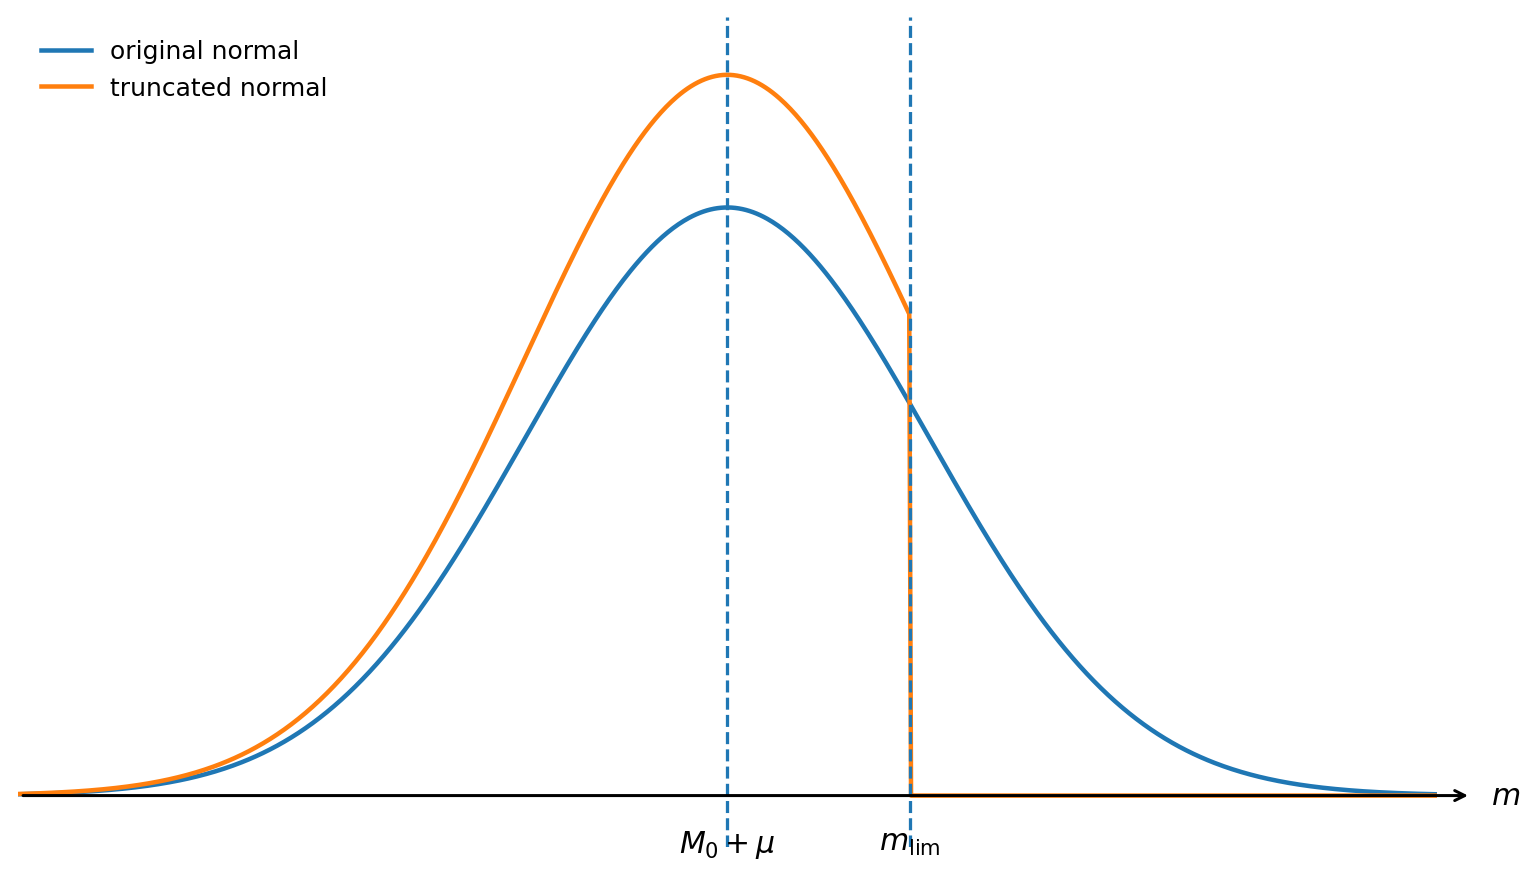
\includegraphics[width=0.5\linewidth]{truncated_normal_explanation_plot_final.png}
    \caption{Truncated Normal}
    \label{fig:truncated_normal}
\end{figure}

Therefore the observed-data likelihood is
\begin{equation*}
    L(\vec\theta)=\prod_{s=1}^N P(m_s\mid I_s=1,\vec\theta).
\end{equation*}


\subsubsection*{A softer selection function}

A natural extension is to allow probabilistic detection rather than a hard cutoff. For example,
\begin{equation*}
    P(I_s=1\mid m_s)
    =
    \Phi\!\left(\frac{m_{\mathrm{lim}}-m_s}{\sigma_{\mathrm{lim}}}\right),
\end{equation*}
where $\sigma_{\mathrm{lim}}$ controls the smoothness of the transition between almost-certain detection and almost-certain non-detection.

Challenge: construct and fit the corresponding observed-data likelihood.

\subsection{Bootstrap}

\subsubsection*{Quantifying uncertainty using the bootstrap}

A frequentist interpretation of uncertainty is the variability of an estimator $g(\vec x)$ under repeated realizations of the experiment, i.e. under repeated random draws of the data $\vec x \sim P(\vec x \mid \vec\theta)$. In other words, we ask: how much would the estimator $g(\vec x)$ change under datasets that we did not actually observe?

For example, the variance of the estimator is
\begin{equation*}
    \mathrm{Var}[g(\vec x)]
    =
    \mathbb{E}\!\left[\bigl(g(\vec x)-\mathbb{E}[g(\vec x)]\bigr)^2\right],
\end{equation*}
where the expectation is taken over repeated draws $\vec x \sim P(\vec x)$.

If $g(\vec x)$ is approximately Gaussian distributed, then an approximate $68\%$ confidence interval is
\begin{equation*}
    g(\vec x)\pm \sqrt{\mathrm{Var}[g(\vec x)]}.
\end{equation*}
More generally, a $(1-\alpha)\%$ confidence interval is an interval $[L(\vec x),U(\vec x)]$ such that it contains the true value at least $(1-\alpha)\%$ of the time under repeated realizations of the experiment. Thus $[L(\vec x),U(\vec x)]$ is a random interval, in contrast to the realised interval $[L(\vec x_{\mathrm{obs}}),U(\vec x_{\mathrm{obs}})]$ computed from one observed dataset $\vec x_{\mathrm{obs}}$.

The \textit{bootstrap} uses the observed dataset to simulate the variability across unobserved, imaginary datasets. A bootstrap sample is obtained by sampling with replacement from the observed dataset to the same sample size.

\begin{example*}[Bootstrap estimation of skewness]
Suppose $X_1,\dots,X_5 \overset{\mathrm{iid}}{\sim} \mathrm{Poisson}(\lambda)$, with pmf
\begin{equation*}
    P(X_i=x_i)=\frac{\lambda^{x_i}e^{-\lambda}}{x_i!}.
\end{equation*}

Suppose we want to estimate the \textit{skewness} of a distribution $P(x)$, i.e. the normalized third central moment
\begin{equation*}
    \mathrm{skewness}
    =
    \frac{\mathbb{E}\!\left[(X-\mu)^3\right]}{(\sigma^2)^{3/2}},
\end{equation*}
where $\mu$ is the true mean and $\sigma^2$ is the true variance.

Define the \textit{sample skewness}
\begin{equation*}
    \hat g(\vec x)
    =
    \frac{\frac{1}{N}\sum_{i=1}^N (x_i-\bar x)^3}
    {\left(\sqrt{\frac{1}{N}\sum_{i=1}^N (x_i-\bar x)^2}\right)^3}.
\end{equation*}

Now suppose we observe $\vec x_{\mathrm{obs}}=(3,8,2,4,5)$ and we form bootstrap datasets by resampling. For instance,
\begin{align*}
    \vec x^{\,b=1} &= (2,5,4,4,4),\\
    \vec x^{\,b=2} &= (2,4,2,8,8),\\
    \vec x^{\,b=3} &= (5,2,8,2,5),
\end{align*}
and so on, up to $\vec x^{\,b=B}$.

For the observed data,
\begin{equation*}
    \hat g^{\,\mathrm{obs}}
    =
    \hat g(\vec x_{\mathrm{obs}})
    =
    0.6927.
\end{equation*}
For the bootstrap samples, compute
\begin{align*}
    \hat g_1 &= \hat g(\vec x^{\,b=1}) = -0.8675,\\
    \hat g_2 &= \hat g(\vec x^{\,b=2}) = 0.2115,\\
    \hat g_3 &= \hat g(\vec x^{\,b=3}) = 0.3930,
\end{align*}
and so on, up to $\hat g_B$.

We can then estimate the sampling variance of the estimator using the empirical variance of the bootstrap replicates,
\begin{equation*}
    \widehat{\mathrm{Var}}(\hat g)
    =
    \widehat{\mathrm{Var}}(\hat g_1,\dots,\hat g_B).
\end{equation*}
In this example, the bootstrap standard error is
\begin{equation*}
    \mathrm{SE}(\hat g)=\sqrt{\widehat{\mathrm{Var}}(\hat g)}\approx 0.635,
\end{equation*}
If $\hat g$ is approximately normal, that is
\begin{align*}
    \frac{\hat g-g}{\mathrm{SE}(\hat g)}\approx\mathcal{N}(0,1),
\end{align*}
then
\begin{equation*}
    \hat g = 0.6927 \pm 0.635.
\end{equation*}
gives an approximate $68\%$ confidence interval. This is because for $Z\sim\mathcal{N}(0,1)$, $\Pr(-1\le Z\le 1)\approx68\%$.




\end{example*}

\section{Regression}

Regression is to fit a function $\mathbb{E}[y\mid x]=f(x;\theta)$
for the conditional mean relation between $y$ and $x$.
There is a large zoo of regression methods. 

\subsection{Ordinary least squares}

\subsubsection*{Linear model}

Suppose we observe $N$ objects and assume the linear model
\begin{equation*}
    y_i=\beta_0+\sum_{j=1}^{k-1}\beta_j x_{ij}+\varepsilon_i,
    \qquad i=1,\dots,N.
\end{equation*}
This can be written in matrix form:
\begin{equation*}
    Y=X\beta+\varepsilon.
\end{equation*}
Assume
\begin{equation*}
    \mathbb{E}[\varepsilon_i]=0,
    \qquad
    \mathrm{Var}(\varepsilon_i)=\sigma^2,
\end{equation*}
so the errors are \textit{homoskedastic}.

\subsubsection*{The OLS estimator}

Ordinary least squares minimizes the residual sum of squares
\begin{align*}
    \mathrm{RSS}
    &=
    \sum_{i=1}^N
    \left(
    y_i-\beta_0-\sum_{j=1}^{k-1}\beta_j x_{ij}
    \right)^2\\
    &=
    (Y-X\beta)^T(Y-X\beta) =\|Y-X\beta\|_2^2
\end{align*}

Differentiating with respect to $\beta$ and setting the gradient equal to zero gives the OLS estimator
\begin{equation*}
    \hat\beta_{\mathrm{OLS}}=(X^TX)^{-1}X^TY.
\end{equation*}

Under the assumptions above, we have
\begin{equation*}
    \mathbb{E}[\hat\beta_{\mathrm{OLS}}]=\beta, \qquad \mathrm{Var}(\hat\beta_{\mathrm{OLS}})
    =
    \sigma^2(X^TX)^{-1}.
\end{equation*}

The \textit{Gauss-Markov} theorem shows that OLS is the \textit{best linear unbiased estimator} (BLUE).

With the OLS estimator $\hat \beta_{\mathrm{OLS}}$, we can estimate $\sigma^2$ by
\begin{equation*}
    \hat\sigma^2
    =
    \frac{1}{N-k}(Y-X\hat\beta)^T(Y-X\hat\beta),
\end{equation*}

\subsection{Weighted least squares: $\chi^2$ minimisation}

\subsubsection*{Known variance components}

Consider the model
$Y_i=f(x_i;\theta)+\varepsilon_i$, $i=1,\dots,N$, where the error variances are known:
$\mathrm{Var}(\varepsilon_i)=\sigma_i^2$.
In the linear case, for example, one may have $f(x_i;\theta)=a+bx_i$, and $\theta=(a,b)$.

Define the \textit{chi-square} function
\begin{equation*}
    \chi^2(\theta)
    =
    \sum_{i=1}^N \frac{\bigl(Y_i-f(x_i;\theta)\bigr)^2}{\sigma_i^2}.
\end{equation*}
An estimator for $\theta$ is obtained by
\begin{equation*}
    \hat{\theta}
    =
    \arg\min_\theta \chi^2(\theta).
\end{equation*}

\subsubsection*{Relation to maximum likelihood}

Suppose
$Y_i=f(x_i;\theta)+\varepsilon_i$
with independent Gaussian errors
$\varepsilon_i \overset{\mathrm{ind}}{\sim} \mathcal{N}(0,\sigma_i^2)$.
Then
\begin{equation*}
    P(y_i\mid x_i;\theta)
    =
    \mathcal{N}\!\left(y_i \mid f(x_i;\theta),\sigma_i^2\right).
\end{equation*}
Hence the likelihood is
\begin{equation*}
    L(\theta)
    =
    \prod_{i=1}^N P(y_i\mid x_i;\theta)
    =
    \prod_{i=1}^N
    \frac{1}{\sqrt{2\pi\sigma_i^2}}
    \exp\!\left[
    -\frac12\frac{(y_i-f(x_i;\theta))^2}{\sigma_i^2}
    \right].
\end{equation*}
Therefore
\begin{align*}
    -2\log L(\theta)
    &=
    \sum_{i=1}^N
    \log(2\pi\sigma_i^2)
    +
    \frac{(y_i-f(x_i;\theta))^2}{\sigma_i^2}\\
    &=
    \chi^2(\theta)
    +
    \sum_{i=1}^N \log(2\pi\sigma_i^2).
\end{align*}
Since the second term does not depend on $\theta$, minimizing $\chi^2(\theta)$ is equivalent to maximizing the likelihood.

\subsubsection*{Unknown variance component}

Now suppose the model contains an additional intrinsic variance component:
$Y_i=f(x_i;\theta)+\varepsilon_{\mathrm{int},i}+\varepsilon_{m,i}$,
where
$\varepsilon_{\mathrm{int},i}\sim \mathcal{N}(0,\sigma_{\mathrm{int}}^2)$
and
$\varepsilon_{m,i}\sim \mathcal{N}(0,\sigma_{m,i}^2)$,
with $\sigma_{m,i}^2$ known but $\sigma_{\mathrm{int}}^2$ unknown.

A naive chi-square extension would be
\begin{equation*}
    \chi^2(\theta,\sigma_{\mathrm{int}}^2)
    =
    \sum_{i=1}^N
    \frac{(Y_i-f(x_i;\theta))^2}{\sigma_{\mathrm{int}}^2+\sigma_{m,i}^2}.
\end{equation*}
However, this is problematic, because $\chi^2(\theta,\sigma_{\mathrm{int}}^2)$ is minimized by taking
$\sigma_{\mathrm{int}}^2\to\infty$.

\subsubsection*{Maximum likelihood with unknown intrinsic variance}

Now,
\begin{equation*}
    P(y_i\mid x_i;\theta,\sigma_{\mathrm{int}}^2)
    =
    \mathcal{N}\!\left(
    y_i \mid f(x_i;\theta),\sigma_{m,i}^2+\sigma_{\mathrm{int}}^2
    \right).
\end{equation*}
Thus the likelihood is
\begin{equation*}
    L(\theta,\sigma_{\mathrm{int}}^2)
    =
    \prod_{i=1}^N
    \frac{1}{\sqrt{2\pi(\sigma_{\mathrm{int}}^2+\sigma_{m,i}^2)}}
    \exp\!\left[
    -\frac12
    \frac{(y_i-f(x_i;\theta))^2}{\sigma_{\mathrm{int}}^2+\sigma_{m,i}^2}
    \right].
\end{equation*}
Hence
\begin{align*}
    -2\log L(\theta,\sigma_{\mathrm{int}}^2)
    &=
    \sum_{i=1}^N
    \frac{(y_i-f(x_i;\theta))^2}{\sigma_{\mathrm{int}}^2+\sigma_{m,i}^2}
    +
    \log\!\bigl[2\pi(\sigma_{\mathrm{int}}^2+\sigma_{m,i}^2)\bigr].
\end{align*}

Now the first term decreases as $\sigma_{\mathrm{int}}^2$ becomes large, but the second term increases. Therefore the maximum likelihood estimate of $\sigma_{\mathrm{int}}^2$ is finite.

The main lesson is that $\chi^2$ is an ad-hoc (made for a particular purpose only) prescription, whereas the likelihood is derived from an explicit probabilistic model. In particular, when variance components are unknown, the likelihood automatically includes the normalization terms that are needed for sensible inference.

\subsubsection*{Model checking}

If the errors are Gaussian, then at the minimizing value $\beta=\hat\beta$, we have
\begin{equation*}
    \chi^2 \sim \chi^2_{N-k}.
\end{equation*}
Hence, for large $N-k$, we should have $\frac{\chi^2}{N-k}\approx 1$, this gives a useful check. 



\subsection{Generalised least squares}
More generally, suppose
\begin{equation*}
    \mathbb{E}[\varepsilon]=0,
    \qquad
    \mathrm{Var}(\varepsilon)=\mathrm{Cov}(\varepsilon,\varepsilon^T)=W,
\end{equation*}
where $W$ is a known covariance matrix. This allows both heteroskedasticity and correlation among the errors.

In this case, we minimise
\begin{equation*}
    \mathrm{RSS}
    =
    (Y-X\beta)^T W^{-1}(Y-X\beta).
\end{equation*}
This gives the \textit{generalised least squares} estimator
\begin{equation*}
    \hat\beta_{\mathrm{GLS}}
    =
    (X^TW^{-1}X)^{-1}X^TW^{-1}Y.
\end{equation*}


Here, 
\begin{equation*}
    \mathbb{E}[\hat\beta_{\mathrm{GLS}}]=\beta, \qquad \mathrm{Var}(\hat\beta_{\mathrm{GLS}})
    =
    (X^TW^{-1}X)^{-1}.
\end{equation*}
Note that OLS and weighted least squares are both special cases of GLS:

\begin{itemize}
    \item OLS corresponds to $W=\sigma^2 I$;
    \item weighted least squares corresponds to diagonal $W=\mathrm{diag}(\sigma_1^2,\dots,\sigma_N^2)$.
\end{itemize}

\subsection{Least squares as maximum likelihood: Gaussian errors}

Assume the linear model
\begin{equation*}
    Y=X\beta+\varepsilon,
\end{equation*}
and suppose
\begin{equation*}
    \varepsilon \sim \mathcal{N}(0,W).
\end{equation*}
Then
\begin{equation*}
    Y\sim \mathcal{N}(X\beta,W).
\end{equation*}
So the likelihood is
\begin{equation*}
    L(\beta)=P(Y\mid \beta,X)=\mathcal{N}(Y\mid X\beta,W).
\end{equation*}

Maximizing this likelihood with respect to $\beta$ is equivalent to minimizing
\begin{equation*}
    (Y-X\beta)^TW^{-1}(Y-X\beta).
\end{equation*}
Hence GLS is exactly the maximum likelihood estimator under Gaussian errors.

\section{Probabilistic Generative Modelling}
A useful way to formulate a statistical model is to describe a \textit{forward} or \textit{generative} process for how the observed data arise from the parameters of interest. In particular, one may introduce intermediate latent variables representing the unobserved true values underlying noisy measurements.

Suppose that for each object $i=1,\dots,N$ we observe $(x_i,y_i)$, but the true latent values are $(\xi_i,\eta_i)$. The model consists of three layers.

\subsection{Generative Model}

\paragraph{Population Distribution}

Assume the latent predictor is drawn from a population distribution
\begin{equation*}
    \xi_i \sim \mathcal{N}(\mu,\tau^2),
\end{equation*}
where
$\psi=(\mu,\tau)$ are population parameters.

\paragraph{Regression model}

Conditional on $\xi_i$, assume the latent response satisfies the linear model
\begin{equation*}
    \eta_i \mid \xi_i \sim \mathcal{N}(\alpha+\beta \xi_i,\sigma^2),
\end{equation*}
where
$\theta=(\alpha,\beta,\sigma^2)$
are regression parameters.

\paragraph{Measurement-error model}

The observed data $(x_i,y_i)$ are noisy measurements of $(\xi_i,\eta_i)$. Assume
\begin{equation*}
    \begin{pmatrix}
        x_i\\
        y_i
    \end{pmatrix}
    \Bigg| \xi_i,\eta_i
    \sim
    \mathcal{N}\!\left(
    \begin{pmatrix}
        \xi_i\\
        \eta_i
    \end{pmatrix},
    \Sigma_i
    \right),
\end{equation*}
with known measurement-error covariance matrix
\begin{equation*}
    \Sigma_i=
    \begin{pmatrix}
        \sigma_{x,i}^2 & 0\\
        0 & \sigma_{y,i}^2
    \end{pmatrix}.
\end{equation*}
More generally, one could allow nonzero off-diagonal covariance if the measurement errors in $x_i$ and $y_i$ are correlated.


\subsection{Formulating likelihood function: marginalising latent variables}

The \textit{observed-data likelihood} is obtained by integrating out the latent variables:
\begin{equation*}
    P(x_i,y_i\mid \theta,\psi)
    =
    \int\!\!\int
    P(x_i,y_i,\xi_i,\eta_i\mid \theta,\psi)\,d\xi_i\,d\eta_i,
\end{equation*}
where $P(x_i,y_i,\xi_i,\eta_i\mid \theta,\psi)$ is called the \textit{complete data likelihood}.

Using the generative model,
\begin{equation*}
    P(x_i,y_i,\xi_i,\eta_i\mid \theta,\psi)
    =
    P(x_i,y_i\mid \xi_i,\eta_i)\,
    P(\eta_i\mid \xi_i,\theta)\,
    P(\xi_i\mid \psi),
\end{equation*}
so
\begin{equation*}
    P(x_i,y_i\mid \theta,\psi)
    =
    \int\!\!\int
    P(x_i,y_i\mid \xi_i,\eta_i)\,
    P(\eta_i\mid \xi_i,\theta)\,
    P(\xi_i\mid \psi)\,d\xi_i\,d\eta_i.
\end{equation*}

If the $N$ observations are conditionally independent, then the full observed-data likelihood is
\begin{equation*}
    P(x,y\mid \theta,\psi)
    =
    \prod_{i=1}^N P(x_i,y_i\mid \theta,\psi).
\end{equation*}



\subsection{Frequentist viewpoint}

In frequentist statistics, there is a distinction between data and parameters: the data are random realisations (observations) of random variables, while the parameters are fixed but unknown constants.


From this viewpoint, the likelihood
\begin{equation*}
    L(\theta,\psi)=P(x,y\mid \theta,\psi)
\end{equation*}
is regarded as a function of the unknown parameters, with the observed data held fixed.


\subsection{Bayesian viewpoint}

In the Bayesian framework, both data and parameters are treated as random variables described jointly by a probability distribution. The data are random variables whose realised values are observed, while the parameters are random variables whose realised values are not observed. Inference is based on conditional probability.

If $D$ denotes the observed data and $\Theta$ denotes the unknown parameters, then Bayes' theorem gives
\begin{equation*}
     P(\Theta\mid D)
    =
    \frac{P(D\mid \Theta)P(\Theta)}{P(D)}.
\end{equation*}


Here, $P(\Theta\mid D)$ is the \textit{posterior}; $P(D\mid \Theta)$ is the \textit{likelihood} or \textit{sampling distribution}; $P(\Theta)$ is the \textit{prior}; $P(D)$ is the normalising constant or \textit{evidence}. Bayesian inference updates prior beliefs about the parameters using the observed data.





\section{Bayesian Inference}


\subsection{Bayesian inference for the generative model}

For the regression model above, the full unknown quantity consists of:
\begin{equation*}
    \Theta=\bigl(\theta,\psi,\{(\xi_i,\eta_i)\}_{i=1}^N\bigr).
\end{equation*}
Given observed data
\begin{equation*}
    D=\{(x_i,y_i)\}_{i=1}^N,
\end{equation*}
Bayesian inference targets the posterior
\begin{equation*}
    P\!\left(\theta,\psi,\{(\xi_i,\eta_i)\}\mid x,y\right).
\end{equation*}

Using Bayes' theorem,
\begin{equation*}
    P\!\left(\theta,\psi,\{(\xi_i,\eta_i)\}\mid x,y\right)
    \propto
    P\!\left(x,y,\{(\xi_i,\eta_i)\}\mid \theta,\psi\right)
    P(\theta,\psi).
\end{equation*}
Equivalently, one may first integrate out the latent variables and work with the observed-data likelihood:
\begin{equation*}
    P(\theta,\psi\mid x,y)
    \propto
    P(x,y\mid \theta,\psi)P(\theta,\psi).
\end{equation*}

So the Bayesian analysis is built on exactly the same generative model and likelihood as before, but now augmented by a prior distribution on the unknown parameters.





\subsection{Simple Gaussian example}\label{subsection:simple_gaussian_example}

Consider the model
\begin{equation*}
    Y_i \overset{\mathrm{iid}}{\sim} \mathcal{N}(\mu,\sigma^2).
\end{equation*}

\subsubsection*{Likelihood and sufficient statistics}

The likelihood is
\begin{align*}
    P(\vec y\mid \mu,\sigma^2)
    &=
    \prod_{i=1}^N \mathcal{N}(y_i\mid \mu,\sigma^2)
    =
    \prod_{i=1}^N \frac{1}{\sqrt{2\pi\sigma^2}}
    \exp\!\left[-\frac{(y_i-\mu)^2}{2\sigma^2}\right]\\
    &=
    (2\pi\sigma^2)^{-N/2}
    \exp\!\left[-\frac{1}{2\sigma^2}\sum_{i=1}^N (y_i-\mu)^2\right]
\end{align*}
Now write $y_i-\mu=(y_i-\bar y)+(\bar y-\mu)$, where
\begin{equation*}
    \bar y=\frac{1}{N}\sum_{i=1}^N y_i
\end{equation*}
is the sample mean. Then
\begin{align*}
    \sum_{i=1}^N (y_i-\mu)^2
    &=
    \sum_{i=1}^N \bigl[(y_i-\bar y)+(\bar y-\mu)\bigr]^2\\
    &=
    \sum_{i=1}^N (y_i-\bar y)^2
    +2(\bar y-\mu)\sum_{i=1}^N (y_i-\bar y)
    +N(\bar y-\mu)^2\\
    &=
    \sum_{i=1}^N (y_i-\bar y)^2
    +N(\bar y-\mu)^2,
\end{align*}
since $\sum_{i=1}^N (y_i-\bar y)=0$. In addition, define the \textit{sample variance} by
\begin{equation*}
    s^2=\frac{1}{N-1}\sum_{i=1}^N (y_i-\bar y)^2,
\end{equation*}
then
\begin{align*}
    P(\vec y\mid \mu,\sigma^2)
    &=
    (2\pi\sigma^2)^{-N/2}
    \exp\!\left[-\frac{1}{2\sigma^2}\sum_{i=1}^N (y_i-\bar y)^2\right]
    \exp\!\left[-\frac{N}{2\sigma^2}(\bar y-\mu)^2\right]\\
    &=
    (2\pi\sigma^2)^{-N/2}
    \exp\!\left[-\frac{(N-1)s^2}{2\sigma^2}\right]
    \exp\!\left[-\frac{N}{2\sigma^2}(\bar y-\mu)^2\right]
\end{align*}


Thus, the likelihood depends on the data only through the \textit{sufficient statistics} $\bar y$ and $s^2$. Thus any two datasets with the same values of $\bar y$ and $s^2$ should yield the same inference.

This gives the \textit{likelihood principle}: all information about the parameters contained in the data is located in the likelihood function.

\subsubsection*{Simple Caussian example with improper prior}

Consider the case where $\sigma^2$ is known but $\mu$ is unknown, and take the \textit{improper prior} $P(\mu)\propto 1$. Then by Bayes' Theorem, ignoring factors constant in $\mu$, we have
\begin{align*}
    P(\mu\mid \vec y)&\propto P(\vec y\mid \mu)P(\mu)\propto P(\vec y\mid \mu)\\
    &\propto
    \exp\!\left[-\frac{N}{2\sigma^2}(\bar y-\mu)^2\right]\\
    &=
    \mathcal{N}\!\left(\mu \mid \bar y,\frac{\sigma^2}{N}\right).
\end{align*}

\subsubsection*{Simple Gaussian example with conjugate prior}

Now again suppose $Y_i \overset{\mathrm{iid}}{\sim} \mathcal{N}(\mu,\sigma^2)$, with $\sigma^2$ known and $\mu$ unknown.

From the likelihood factorization above,
\begin{equation*}
    P(\vec y\mid \mu)
    \propto
    \exp\!\left[-\frac{N}{2\sigma^2}(\bar y-\mu)^2\right].
\end{equation*}

A \textit{conjugate prior} means a prior chosen so that, after multiplying by the likelihood, the posterior stays in the same distribution family as the prior. Here, take a conjugate prior
\begin{equation*}
    P(\mu)=\mathcal{N}(\mu\mid \mu_0,\tau_0^2),
\end{equation*}
or equivalently
\begin{equation*}
    \mu \sim \mathcal{N}(\mu_0,\tau_0^2),
\end{equation*}
where $\mu_0$ is the prior mean and $\tau_0^2$ is the prior variance.

Then the posterior is
\begin{equation*}
    P(\mu\mid \vec y)\propto P(\vec y\mid \mu)P(\mu).
\end{equation*}
Substituting the Gaussian forms,
\begin{equation*}
    P(\mu\mid \vec y)
    \propto
    \exp\!\left[-\frac{N}{2\sigma^2}(\bar y-\mu)^2\right]
    \exp\!\left[-\frac{1}{2\tau_0^2}(\mu-\mu_0)^2\right].
\end{equation*}
Direct calculation shows that
\begin{equation*}
    P(\mu\mid \vec y)=\mathcal{N}(\mu\mid \mu_N,\tau_N^2),
\end{equation*}
where
\begin{equation*}
    \mu_N
    =
    \frac{\dfrac{1}{\tau_0^2}\mu_0+\dfrac{N}{\sigma^2}\bar y}
    {\dfrac{1}{\tau_0^2}+\dfrac{N}{\sigma^2}}
\end{equation*}
and
\begin{equation*}
    \frac{1}{\tau_N^2}
    =
    \frac{1}{\tau_0^2}+\frac{N}{\sigma^2}.
\end{equation*}

Here, the posterior mean is a weighted average of the prior mean and the sample mean, while the posterior precision is the sum of the prior precision and the likelihood precision. (precision is the inverse of variance)

For fixed prior variance $\tau_0^2$, as $N\to\infty$,
\begin{equation*}
    \mu_N\to \bar y,
    \qquad
    \tau_N^2\to \frac{\sigma^2}{N}.
\end{equation*}
So for large samples the data dominate the prior.




\subsection{Multi-parameter Bayesian inference: Gaussian example}\label{subsection:multi-parameter_bayesian_inference:gaussian}

Consider the Gaussian model
\begin{equation*}
    y_i \overset{\mathrm{iid}}{\sim} \mathcal{N}(\mu,\sigma^2),
    \qquad i=1,\dots,n.
\end{equation*}
Now both $\mu$ and $\sigma^2$ are unknown.
Consider the improper priors $P(\mu)\propto 1$ and $P(\sigma^2)\propto \sigma^{-2}$, equivalently $P(\log \sigma^2)\propto 1$, for $\sigma^2>0$.

The likelihood is
\begin{equation*}
    P(y\mid \mu,\sigma^2)
    =
    (2\pi\sigma^2)^{-n/2}
    \exp\!\left[
    -\frac{(n-1)s^2}{2\sigma^2}
    \right]
    \exp\!\left[
    -\frac{n}{2\sigma^2}(\bar y-\mu)^2
    \right],
\end{equation*}
where $\bar y$ and $s^2$ are the sample mean and sample variance, and they are sufficient statistics.

Hence the joint posterior is
\begin{align*}
    P(\mu,\sigma^2\mid y)
    &\propto P(y\mid \mu, \sigma^2)\times P(\mu)P(\sigma^2)
   \\
    &\propto (\sigma^2)^{-n/2-1}
    \exp\!\left[
    -\frac{(n-1)s^2}{2\sigma^2}
    \right]
    \exp\!\left[
    -\frac{n}{2\sigma^2}(\bar y-\mu)^2
    \right]
\end{align*}

\subsubsection*{Conditional posterior}

Condition on $\sigma^2$ (take $\sigma^2$ as a constant), we have
\begin{equation*}
    P(\mu\mid \sigma^2,y)
    \propto 
    \exp\!\left[
    -\frac{n}{2\sigma^2}(\bar y-\mu)^2
    \right],
\end{equation*}
so
\begin{equation*}
    P(\mu\mid \sigma^2,y)= \mathcal{N}\!\left(\mu\mid \bar y,\frac{\sigma^2}{n}\right).
\end{equation*}

\subsubsection*{Marginal Posterior}
Integrating out $\mu$ gives
\begin{equation*}
    P(\sigma^2\mid y)=\int  P(\mu,\sigma^2\mid y) d\mu
    =\mathrm{Inv}\text{-}\chi^2(\sigma^2\mid n-1,s^2).
\end{equation*}
Integrating out $\sigma^2$ gives
\begin{equation*}
    P(\mu\mid y)=\int  P(\mu,\sigma^2\mid y) d\sigma^2
    \propto
    \left[
    1+\frac{n(\mu-\bar y)^2}{(n-1)s^2}
    \right]^{-n/2}
    =
    t_{n-1}\!\left(\mu\mid \bar y,\frac{s^2}{n}\right).
\end{equation*}

\subsubsection*{Inverse-chi-squared and inverse-gamma}

The \textit{inverse-chi-squared} distribution is defined as
\begin{equation*}
    \mathrm{Inv}\text{-}\chi^2(\theta\mid \nu,s^2)
    \propto
    \theta^{-(\nu/2+1)}
    \exp\!\left(-\frac{\nu s^2}{2\theta}\right),
    \qquad \theta>0.
\end{equation*}
This is the same family as the \textit{inverse-gamma} distribution,
\begin{equation*}
    \mathrm{Inv}\text{-}\Gamma(\theta\mid \alpha,\beta)
    \propto
    \theta^{-(\alpha+1)}
    \exp(-\beta/\theta),
    \qquad \theta>0,
\end{equation*}
with the parameters $\alpha=\nu/2$ and $\beta=\nu s^2/2$.

\subsubsection*{Student-$t$ distribution}

The Student-\(t\) distribution with \textit{location} \(\mu\), \textit{scale} \(\tau^2\), and \textit{degrees of freedom} \(\nu\) has density
\begin{equation*}
    t_\nu(\theta\mid \mu,\tau^2)
    \propto
    \left[
    1+\frac{1}{\nu}\frac{(\theta-\mu)^2}{\tau^2}
    \right]^{-(\nu+1)/2}.
\end{equation*}
In the Gaussian example above, the marginal posterior for \(\mu\) has exactly this form.

\subsection{Bayesian computation}

In Bayesian inference, the answer is the full posterior density \(P(\theta\mid D)\), which describes the state of knowledge after seeing the data. Numerical summaries such as posterior means, modes, and \(95\%\) highest posterior density regions are only summaries of this full object.

Many quantities of interest are posterior expectations of the form
\begin{equation*}
    \mathbb{E}[f(\theta)\mid D]
    =
    \int f(\theta)P(\theta\mid D)\,d\theta,
\end{equation*}
which may be computationally difficult.

When analytic calculations are not available, Bayesian computation aims to map out or sample from the posterior and estimate such expectations numerically. Common methods include:
\begin{itemize}
    \item Markov chain Monte Carlo;
    \item Gibbs sampling;
    \item nested sampling;
    \item importance sampling.
\end{itemize}

As always, all models are wrong, though some are useful. Even exact computation under a poor model can still lead to poor scientific conclusions.


\section{Importance Sampling}

\subsection{Direct sampling and Monte Carlo integration}

In Bayesian inference, the full answer is the posterior density $P(\theta\mid D)$. Any numerical estimates summarise the posterior, e.g. posterior mean, modes, variance, and credible regions are only summaries of this posterior.

A common task is to compute posterior expectations of the form
\begin{equation*}
    I=\mathbb{E}[f(\theta)\mid D]=\int f(\theta)\,P(\theta\mid D)\,d\theta.
\end{equation*}
When we can draw samples $\theta_1,\dots,\theta_m \overset{\mathrm{iid}}{\sim} P(\theta\mid D)$, we approximate this by the \textit{Monte Carlo estimator}
\begin{equation*}
    \hat I=\frac{1}{m}\sum_{i=1}^m f(\theta_i).
\end{equation*}
Here $m$ is the Monte Carlo sample size, not the data sample size.

By the law of large numbers, $\hat I$ converges to $\mathbb{E}[f(\theta)\mid D]=I$ as $m\to\infty$. Its variance is
\begin{align*}
    \mathrm{Var}(\hat I)
    &= \mathrm{Cov}(\hat I,\hat I)\\
    &= \mathrm{Cov}\!\left(\frac{1}{m}\sum_{i=1}^m f(\theta_i),\frac{1}{m}\sum_{j=1}^m f(\theta_j)\right)\\
    &= \frac{1}{m^2}\sum_{i=1}^m\sum_{j=1}^m \mathrm{Cov}(f(\theta_i),f(\theta_j)).
\end{align*}
Since the draws are iid, the cross-covariances vanish, so
\begin{equation*}
    \mathrm{Var}(\hat I)=\frac{1}{m}\mathrm{Var}(f(\theta)).
\end{equation*}
Thus the Monte Carlo error (standard error) scales as $m^{-1/2}$.

For large $m$, the central limit theorem gives
\begin{equation*}
    \hat I \approx \mathcal{N}\!\left(\mathbb{E}[f(\theta)\mid D],\frac{\mathrm{Var}(f(\theta))}{m}\right).
\end{equation*}
In practice we estimate $\mathrm{Var}(f(\theta))$ by the sample variance of $\{f(\theta_i)\}_{i=1}^m$:
\begin{equation*}
    \widehat{\mathrm{Var}}(f(\theta))
    =
    \frac{1}{m-1}\sum_{i=1}^m \bigl(f(\theta_i)-\hat I\bigr)^2.
\end{equation*}
\begin{example*} Some common choices of $f$ are:

    \begin{itemize}
    \item posterior mean: take $f(\theta)=\theta$;
    \item posterior variance: take $f(\theta)=(\theta-\mathbb{E}[\theta\mid D])^2$;
    \item posterior probability of an interval $[a,b]$: take $f(\theta)=I_{[a,b]}(\theta)$.
\end{itemize}
\end{example*}


\subsubsection*{Direct sampling in a Gaussian example}

Recall the Gaussian model
$y_i \overset{\mathrm{iid}}{\sim} \mathcal{N}(\mu,\sigma^2)$, $i=1,\dots,n$,
with prior $P(\mu)\propto 1$ and $P(\sigma^2)\propto \sigma^{-2}$ for $\sigma^2>0$. The joint posterior factorizes as
\begin{equation*}
    P(\mu,\sigma^2\mid y)=P(\mu\mid \sigma^2,y)\,P(\sigma^2\mid y),
\end{equation*}
where
$P(\mu\mid \sigma^2,y)=\mathcal{N}(\mu\mid \bar y,\sigma^2/n)$
and
$P(\sigma^2\mid y)=\mathrm{Inv}\text{-}\chi^2(\sigma^2\mid n-1,s^2)$.

This immediately suggests a \textit{direct sampling} algorithm:
\begin{enumerate}
    \item draw $\sigma_i^2 \sim P(\sigma^2\mid y)$;
    \item draw $\mu_i \mid \sigma_i^2 \sim P(\mu\mid \sigma_i^2,y)$.
\end{enumerate}
Then $(\mu_i,\sigma_i^2)\sim P(\mu,\sigma^2\mid y)$ is a joint draw from the posterior.

Once we have many such draws, posterior summaries can be computed directly from the samples, without having to derive marginal densities analytically. 

% Figure note:
% The joint scatterplot of posterior draws and the marginal histograms are conceptually useful.
% They show that direct sampling gives both the joint posterior and the marginals without
% analytic integration.

\subsection{Kernel density estimation}

Given posterior samples $\theta_1,\dots,\theta_m \overset{\mathrm{iid}}{\sim} P(\theta\mid D)$, we may want a smooth estimate of the posterior density. A \textit{kernel density estimate} is  obtained by centering a smooth kernel at each sample point and averaging. Here, a \textit{kernel} is generally taken to be a probability density function that is symmetric. 

Using Gaussian kernels, the KDE is
\begin{equation*}
    \hat P(\theta\mid D)
    =
    \frac{1}{m}\sum_{i=1}^m \mathcal{N}(\theta\mid \theta_i,\mathrm{bw}^2),
\end{equation*}
where $\mathrm{bw}$ is the bandwidth. Since each Gaussian kernel integrates to $1$,
\begin{equation*}
    \int \hat P(\theta\mid D)\,d\theta
    =
    \frac{1}{m}\sum_{i=1}^m \int \mathcal{N}(\theta\mid \theta_i,\mathrm{bw}^2)\,d\theta
    = 1.
\end{equation*}
So the KDE is automatically normalized.

A common rule-of-thumb for the bandwidth is \textit{Silverman’s rule}:
\begin{equation*}
    \mathrm{bw}
    =
    \left(\frac{4\hat\sigma^5}{3m}\right)^{1/5},
\end{equation*}
where $\hat\sigma^2$ is the sample variance of the draws.

The practical picture is simple: each sample point contributes one Gaussian bump, and the KDE is obtained by summing all these bumps and normalizing. This provides a smooth visual approximation to the posterior density.

\subsection{Summarising posterior uncertainties}

A simple posterior summary is the posterior mean or posterior median together with the posterior standard deviation. If the posterior is Gaussian, then mean $\pm$ one posterior standard deviation contains about $68\%$ posterior probability. To see this, let $Z\sim\mathcal{N}(0,1)$, then
\begin{equation*}
    \Pr(-1\le Z\le 1)\approx68\%.
\end{equation*}

For non-Gaussian posteriors, however, this need not hold.

\subsubsection*{Credible intervals}

A \textit{credible interval} is a set of parameter values containing a specified amount of posterior probability. Unlike a frequentist confidence interval, it is a direct probability statement about the parameter conditional on the data.

One common choice is a quantile-based interval. For example, a $68\%$ central credible interval is given by the $16\%$ and $84\%$ posterior quantiles. This is easy to compute from posterior samples.

Such intervals are not unique: different sets may contain the same posterior probability.

\subsubsection*{Highest posterior density regions}

A particularly useful credible region is the \textit{highest posterior density} (\textit{HPD}) region. Informally, it is the narrowest region containing a fixed posterior probability.

Formally, for posterior probability level $X$, the HPD region is a set $\Theta$ such that
\begin{equation*}
    \int_{\Theta} P(\theta\mid D)\,d\theta = X,
\end{equation*}
and there exists a threshold $\rho$ with
\begin{equation*}
    P(\theta\mid D)\ge \rho
    \qquad \text{for all } \theta\in \Theta.
\end{equation*}
Equivalently,
\begin{equation*}
    \Theta = \{\theta: P(\theta\mid D)\ge \rho\},
\end{equation*}
where $\rho$ is chosen so that the enclosed posterior probability is exactly $X$.

For a unimodal posterior, the HPD region is typically a single interval. For a multimodal posterior, the HPD region may be disconnected: it can be the union of several disjoint intervals. This is one advantage of the HPD definition over central quantile intervals.

\begin{figure}
    \centering
    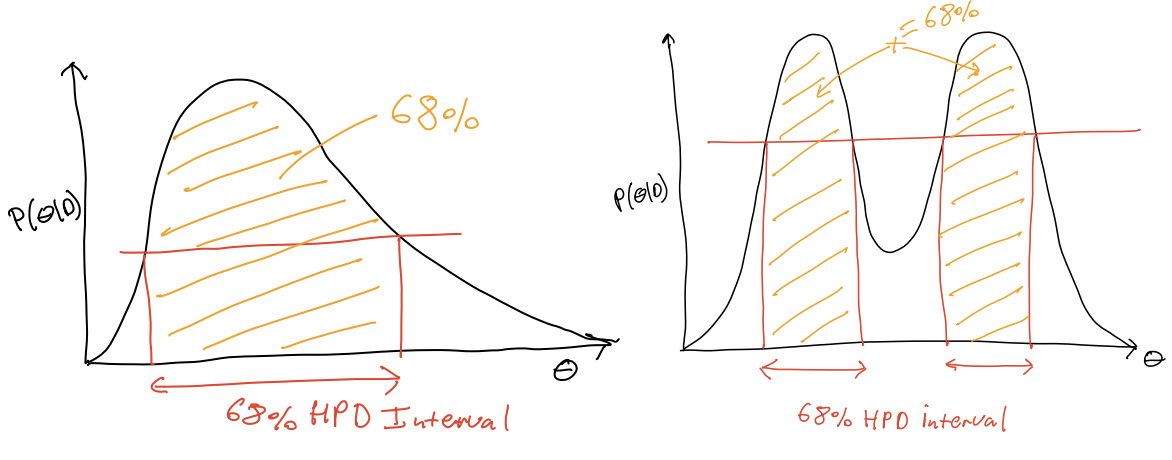
\includegraphics[width=0.5\linewidth]{Multimodal_HPD.png}
    \caption{68\% HPD intervals for unimodal and multimodal posteriors}
    \label{fig:HPD}
\end{figure}

\subsubsection*{What if direct sampling is impossible?}

If we cannot directly sample $\theta_i\sim P(\theta\mid D)$, there are two broad strategies:
\begin{itemize}
    \item \textit{importance sampling}: sample from an easier tractable density $Q(\theta)$ and weight by $P(\theta\mid D)/Q(\theta)$;
    \item \textit{posterior simulation}: use algorithms such as Markov chain Monte Carlo, nested sampling, or related methods to generate approximate draws from the posterior in the long run.
\end{itemize}

So the main computational message is:
\begin{equation*}
    \mathbb{E}[f(\theta)\mid D]
    =
    \int f(\theta)P(\theta\mid D)\,d\theta
    \approx
    \frac{1}{m}\sum_{i=1}^m f(\theta_i),
\end{equation*}
provided the samples $\theta_i$ are produced in a way that correctly represents the posterior.

\subsection{Importance sampling}

Suppose we want to compute
\begin{equation*}
    I=\mathbb{E}_{P}[f(\theta)]=\int f(\theta)\,P(\theta)\,d\theta,
\end{equation*}
where $P(\theta)$ is a target density, for example the posterior $P(\theta|D)$. Sometimes $P(\theta)$ is \textit{intractable} for direct sampling: we cannot easily draw $\theta_i\sim P(\theta)$, even though we can evaluate $P(\theta_i)$ pointwise.

The idea of \textit{importance sampling} is to introduce an easier \textit{importance function} $Q(\theta)$ such that
\begin{itemize}
    \item it is easy to draw samples $\theta_i\sim Q(\theta)$;
    \item we can evaluate $Q(\theta_i)$;
    \item $Q(\theta)>0$ wherever $P(\theta)>0$.
\end{itemize}

Then rewrite
\begin{align*}
    I
    &= \int f(\theta)\,\frac{P(\theta)}{Q(\theta)}\,Q(\theta)\,d\theta\\
    &= \mathbb{E}_{Q}\!\left[f(\theta)\frac{P(\theta)}{Q(\theta)}\right].
\end{align*}
So if $\theta_1,\dots,\theta_m \overset{\mathrm{iid}}{\sim} Q(\theta)$, we estimate $I$ by
\begin{equation*}
    \hat I^*
    =
    \frac{1}{m}\sum_{i=1}^m f(\theta_i)\frac{P(\theta_i)}{Q(\theta_i)}
    =
    \frac{1}{m}\sum_{i=1}^m f(\theta_i)w_i^*,
\end{equation*}
where
\begin{equation*}
    w_i^*=\frac{P(\theta_i)}{Q(\theta_i)}
\end{equation*}
are the \textit{importance weights}.

This estimator is unbiased:
\begin{align*}
    \mathbb{E}_{Q}[\hat I^*]
    &= \frac{1}{m}\sum_{i=1}^m \mathbb{E}_{Q}[f(\theta_i)w_i^*]\\
    &= \frac{1}{m}\sum_{i=1}^m \int f(\theta)\frac{P(\theta)}{Q(\theta)}Q(\theta)\,d\theta\\
    &= \frac{1}{m}\sum_{i=1}^m \int f(\theta)P(\theta)\,d\theta= \frac{1}{m}\sum_{i=1}^m I= I.
\end{align*}
Its variance is
\begin{equation*}
    \mathrm{Var}_Q(\hat I^*)
    =\frac{1}{m^2}\sum_{i=1}^m\mathrm{Var}_Q(f(\theta_i)w_i^*)
    =
    \frac{1}{m}\mathrm{Var}_{Q}\!\left(f(\theta)\frac{P(\theta)}{Q(\theta)}\right),
\end{equation*}
which in practice can be estimated from the empirical variance of the weighted sample values $\{f(\theta_i)w_i^*\}$.

\begin{remark}
    Notice that we cannot calculate
    \begin{equation*}
        w_i^*=\frac{P(\theta_i)}{Q(\theta_i)}
    \end{equation*}
    if we know nothing about $P(\theta_i)$. However, in Bayesian problems, we can evaluate the posterior $P(\theta\mid D)$ up to a multiplicative constant. This leads to the idea of self-normalised importance sampling.
\end{remark}


\subsubsection*{Self-normalised importance sampling}

In Bayesian problems, we often know the posterior only up to proportionality. Write
\begin{equation*}
    P(\theta)=\frac{\tilde P(\theta)}{Z_P},
    \qquad
    Z_P=\int \tilde P(\theta)\,d\theta,
\end{equation*}
where $\tilde P(\theta)$ is an unnormalised density, for example $\tilde P(\theta)=L(\theta)\pi(\theta)$, where $L$ is the likelihood and $\pi$ is the prior.

The problem is that $Z_P$ is unknown, so $P(\theta)$ cannot be evaluated exactly. We still want to estimate
\begin{equation*}
    I=\mathbb{E}_{P}[f(\theta)]=\int f(\theta)P(\theta)\,d\theta.
\end{equation*}
Substituting $P(\theta)=\tilde P(\theta)/Z_P$ and multiplying and dividing by $Q(\theta)$ gives
\begin{align*}
    I
    &= \frac{\int f(\theta)\tilde P(\theta)\,d\theta}{\int \tilde P(\theta)\,d\theta}= \frac{\int f(\theta)\dfrac{\tilde P(\theta)}{Q(\theta)}Q(\theta)\,d\theta}
    {\int \dfrac{\tilde P(\theta)}{Q(\theta)}Q(\theta)\,d\theta}=\frac{\mathbb{E}_Q\left[f(\theta)\frac{\tilde P(\theta)}{Q(\theta)}\right]}{\mathbb{E}_Q\left[\frac{\tilde P(\theta)}{Q(\theta)}\right]}.
\end{align*}
If $\theta_1,\dots,\theta_m \overset{\mathrm{iid}}{\sim} Q(\theta)$, define the \textit{unnormalised importance weights}
\begin{equation*}
    \tilde w_i=\frac{\tilde P(\theta_i)}{Q(\theta_i)}.
\end{equation*}
Then we can estimate $I$ with the \textit{self-normalised importance sampling estimator} defined as
\begin{equation*}
    \hat I
    =
    \frac{\sum_{i=1}^m f(\theta_i)\tilde w_i}{\sum_{i=1}^m \tilde w_i}
    =
    \sum_{i=1}^m f(\theta_i)w_i,
\end{equation*}
where the \textit{self-normalised weights} are
\begin{equation*}
    w_i=\frac{\tilde w_i}{\sum_{j=1}^m \tilde w_j}
    =
    \frac{\tilde P(\theta_i)/Q(\theta_i)}
    {\sum_{j=1}^m \tilde P(\theta_j)/Q(\theta_j)}.
\end{equation*}

This construction also works if $Q$ is itself only known up to a normalising constant, because any multiplicative constant in $Q$ cancels between numerator and denominator.

The cost is that $\hat I$ is slightly biased, with
\begin{equation*}
    \mathbb{E}[\hat I]=I+\mathcal{O}(m^{-1}).
\end{equation*}


\subsubsection*{Choosing a good importance function}

(See example sheet 2) The theoretical minimum-variance importance function is 
\begin{equation*}
    Q^*(\theta)
    =
    \frac{|f(\theta)|P(\theta)}
    {\int |f(\theta)|P(\theta)\,d\theta}.
\end{equation*}
In practice this is rarely usable, because if we can't sample from $P(\theta)$, we probably can't sample from $|f(\theta)|P(\theta)$ either.


The practical guideline is instead:
\begin{itemize}
    \item choose $Q$ with support wherever $P$ is nonzero,
    \item make $Q$ similar in shape to $|f(\theta)|P(\theta)$.
\end{itemize}
The aim is to keep the weights roughly constant. Large variability in the weights leads to unstable estimates and small effective sample size.


\subsubsection*{Effective sample size}

The \textit{effective sample size} (\textit{ESS}) is a convenient diagnostic. 
\begin{equation*}
    \mathrm{ESS}
    =
    \frac{m}{1+\widehat{\mathrm{Var}}\!\left(\{w_i^*\}\right)},
\end{equation*}
where $w_i^*=P(\theta_i)/Q(\theta_i)$ are the importance weights.

The interpretation is simple: if all weights are similar, then ESS is close to $m$; if a few weights dominate, then ESS is much smaller than $m$. In that case, only a small number of samples contribute materially to the estimate.

\begin{remark}
    Importance sampling is conceptually simple and often very effective when: the target density can be evaluated pointwise;
    a good proposal $Q$ is available;
    the dimension is not too large;
    the importance weights are not too variable. When these conditions fail, one often turns to Markov chain Monte Carlo or other posterior simulation methods instead.
\end{remark}



\subsubsection*{Example: Use the prior itself as the importance function}

Let $d$ be the (noisy) measurement of kinematic properties of our Milky Way satellite's prperties; $x$ be the latent (true) values of satellite properties; $m=\log_{10}[\text{mass of central galaxy}]$. We aim to estimate quantities of the form
\begin{equation*}
    \mathbb{E}[f(m)\mid d]=\int f(m)\,P(m\mid d)\,dm.
\end{equation*}
For example, choosing $f(m)=m$ gives the posterior mean, while choosing $f(m)=\bigl(m-\mathbb{E}[m\mid d]\bigr)^2$ gives the posterior variance.

Since
\begin{equation*}
    P(m\mid d)=\int P(x,m\mid d)\,dx,
\end{equation*}
we can write
\begin{equation*}
    \mathbb{E}[m\mid d]
    =
    \iint m\,P(x,m\mid d)\,dx\,dm.
\end{equation*}
By Bayes' theorem,
\begin{equation*}
    P(x,m\mid d)
    = \frac{P(d\mid x,m)\,P(x,m)}
    {\iint P(d\mid x,m)\,P(x,m)\,dx\,dm}
\end{equation*}
where $P(d\mid x,m)$ is the (Gaussian) measurement likelihood, and $P(x,m)$ is the physical prior. 
If the data $d$ depend on the parameter only through the latent quantity $x$, then
\begin{equation*}
    P(d\mid x,m)=P(d\mid x),
\end{equation*}
so
\begin{equation*}
    P(x,m\mid d)
    =
    \frac{P(d\mid x)\,P(x,m)}
    {\iint P(d\mid x)\,P(x,m)\,dx\,dm}.
\end{equation*}

A common problem is that the prior $P(x,m)$ may be \textit{intractable}: we can sample from it, but we cannot evaluate it analytically. Now, suppose a simulator generates iid draws
\begin{equation*}
    (x_j,m_j)\overset{\mathrm{iid}}{\sim} P(x,m),
    \qquad j=1,\dots,n.
\end{equation*}
Then we can choose the importance function to be the prior itself
\begin{equation*}
    Q(x,m)=P(x,m).
\end{equation*}
In this case, since $(x_j,m_j)\overset{\mathrm{iid}}{\sim} P(x,m)$, we can estimate the posterior expectation by
\begin{align*}
    \mathbb{E}[m\mid d]
    =
    \frac{\iint m\,P(d\mid x)\,P(x,m)\,dx\,dm}
    {\iint P(d\mid x)\,P(x,m)\,dx\,dm}\approx
    \frac{\frac{1}{n}\sum_{j=1}^n m_j\,P(d\mid x_j)}
    {\frac{1}{n}\sum_{j=1}^n P(d\mid x_j)}=
    \sum_{j=1}^n m_j w_j,
\end{align*}
where the weights are
\begin{equation*}
    w_j=
    \frac{P(d\mid x_j)}
    {\sum_{k=1}^n P(d\mid x_k)}.
\end{equation*}
Thus the likelihood alone determines the weights, because the importance function has been chosen equal to the prior.




\subsection{Weighted kernel density estimation}

For posterior samples $\theta_1,\dots,\theta_m \overset{\mathrm{iid}}{\sim} P(\theta\mid D)$, recall that the KDE is 

\begin{equation*}
    \hat P(\theta\mid D)
    =
    \frac{1}{m}\sum_{i=1}^m \mathcal{N}(\theta\mid \theta_i,\mathrm{bw}^2),
\end{equation*}
where bw is the band width.

Now, under the importance sampling context, we sample $\theta_1,\dots,\theta_m \overset{\mathrm{iid}}{\sim} Q(\theta)$ for some importance function $Q$. Instead of $\frac{1}{m}$, we have normalized importance weights $w_1,\dots,w_m$, where
\begin{equation*}
    \sum_{s=1}^m w_s=1.
\end{equation*}
A \textit{weighted kernel density estimate} of the posterior density is
\begin{equation*}
    \mathrm{wkde}(\theta)
    =
    \sum_{s=1}^m w_s\,\mathcal{N}(\theta\mid \theta_s,\mathrm{bw}^2),
\end{equation*}
where $\mathrm{bw}$ is the bandwidth.
WKDE also gives a smooth approximation to the posterior density.

\subsubsection*{Choice of importance weights}
\begin{align*}
    P(\theta|D)=\frac{P(D|\theta)P(\theta)}{P(D)}=\frac{P(D|\theta)P(\theta)}{\int P(D|\theta)P(\theta) d\theta}
\end{align*}
Suppose we sample $\theta_1,\dots,\theta_m \overset{\mathrm{iid}}{\sim} Q(\theta)$ for some importance function $Q$. We have that 
\begin{align*}
    P(D|\theta)P(\theta)=\int\delta(\theta-\theta')P(D|\theta')P(\theta')d\theta',
\end{align*}
so
\begin{align*}
     P(\theta|D)&=\frac{\int\delta(\theta-\theta')P(D|\theta')P(\theta')d\theta'}{\int P(D|\theta')P(\theta') d\theta'}\\
     &=\frac{\int\delta(\theta-\theta')P(D|\theta')\frac{P(\theta')}{Q(\theta')}Q(\theta')d\theta'}{\int P(D|\theta')\frac{P(\theta')}{Q(\theta')}Q(\theta') d\theta'}\\
     &=\frac{\mathbb{E}_{\theta'\sim Q(\theta')}[\delta(\theta-\theta')P(D|\theta')\frac{P(\theta')}{Q(\theta')}]}{\mathbb{E}_{\theta'\sim Q(\theta')}[P(D|\theta')\frac{P(\theta')}{Q(\theta')}]}\\
     &\approx\frac{\frac{1}{m}\sum_{i=1}^m \delta(\theta-\theta_i)P(D|\theta_i)\frac{P(\theta_i)}{Q(\theta_i)} }{\frac{1}{m}\sum_{i=1}^m P(D|\theta_i)\frac{P(\theta_i)}{Q(\theta_i)} }.
\end{align*}

In KDE, we approximate the point mass $\delta(\theta-\theta_i)$ by $\mathcal{N}(\theta\mid\theta_i,\mathrm{bw}^2)$, so we get the approximation
\begin{equation*}
    \hat P(\theta\mid D) = \sum_{i=1}^m w_i \mathcal{N}(\theta\mid\theta_i,\mathrm{bw}^2),
\end{equation*}
where
\begin{equation*}
    w_i = \frac{P(D|\theta_i)\frac{P(\theta_i)}{Q(\theta_i)} }{\sum_{j=1}^m P(D|\theta_j)\frac{P(\theta_j)}{Q(\theta_j)} }.
\end{equation*}
This is the same $w_i$ as before. 

\subsubsection*{Bandwidth choice}

A common rule of thumb is \textit{Silverman's rule}:
\begin{equation*}
    \mathrm{bw}
    =
    \left(\frac{4\hat\sigma^5}{3n}\right)^{1/5},
\end{equation*}
where $\hat\sigma^2$ is an estimate of the posterior variance. In importance sampling, we often replace $n$ by the effective sample size.


\section{Markov Chain Monte Carlo}

For a small number $p$ of parameters, we can evaluate posterior on a $p-$dimensional grid. This is inefficient for $p>3$. Realistic models often involve many parameters, and direct evaluation or direct simulation becomes infeasible. In this setting, \textit{Markov chain Monte Carlo} (\textit{MCMC}) is the standard computational workhorse. The idea of MCMC is to generate a correlated sequence of random variables whose limiting distribution is the posterior.

The aim is still to compute expectations of the form
\begin{equation*}
    \mathbb{E}[f(\theta)\mid D]=\int f(\theta)P(\theta\mid D)\,d\theta.
\end{equation*}

MCMC constructs a Markov Chain whose distribution converges to the posterior distribution. That is, the stationary distribution is the posterior distribution.

\subsection{A sketch of MCMC theory}

\subsubsection*{Markov chains}

A \textit{Markov chain} is a sequence of random variables
\begin{equation*}
    \theta^0,\theta^1,\dots,\theta^{t-1},\theta^t \in \Theta,
\end{equation*}
with the \textit{Markov property}
\begin{equation*}
    P(\theta^t \mid \theta^{t-1},\dots,\theta^1,\theta^0)
    =
    P(\theta^t \mid \theta^{t-1}),
\end{equation*}
where $\Theta$ is the state space (parameter space).

If the chain starts from an initial distribution $\pi_0(\theta^0)$ and has \textit{transition probabilities}
\begin{equation*}
    T_t(\theta^{t-1}\to \theta^t)
    =
    P(\theta^t\mid \theta^{t-1}),
\end{equation*}
then the joint distribution is
\begin{align*}
    P(\theta^t,\theta^{t-1},\dots,\theta^1,\theta^0)
    &=
    P(\theta^t\mid \theta^{t-1})P(\theta^{t-1}\mid \theta^{t-2})\cdots P(\theta^1\mid \theta^0)P(\theta^0)\\
    &=
    \pi_0(\theta^0)\,T_1(\theta^0\to \theta^1)\cdots T_t(\theta^{t-1}\to \theta^t).
\end{align*}

If the transition rule does not depend on time, that is,
\begin{equation*}
    T_t(\theta\to \theta')=T(\theta\to \theta'),
\end{equation*}
then the chain is called \textit{time homogeneous}.

In the time homogeneous case, the \textit{marginal distribution} at time $t$ is
\begin{equation*}
    P(\theta^t)
    =
    \int \pi_0(\theta^0)\,T(\theta^0\to \theta^1)\cdots T(\theta^{t-1}\to \theta^t)\,d\theta^0\cdots d\theta^{t-1}.
\end{equation*}

\subsubsection*{Goal of MCMC}

The goal of MCMC is to construct a Markov chain whose limiting distribution is the desired target posterior. 

A distribution is \textit{stationary} if when the chain starts with initial distribution $\pi_{\text{stat}}$, it stays distributed as $\pi_{\mathrm{stat}}$ forever. In time homogeneous case, stationary distributions are defined by the time-independent transition probabilities. 

A \textit{limiting distribution} is defined as
\begin{equation*}
    \pi_{\mathrm{lim}}(\theta)
    :=
    \lim_{t\to\infty} P(\theta^t=\theta).
\end{equation*}
In general, every limiting distribution is stationary, but not every stationary distribution is necessarily the limiting distribution from a given start.

In MCMC, we want to find Markov chains such that
\begin{equation*}
    \pi_{\mathrm{lim}}(\theta)=
    \pi_{\mathrm{stat}}(\theta)=
    \pi_{\mathrm{post}}(\theta),
\end{equation*}
where $\pi_{\mathrm{post}}$ is the posterior distribution. 

\subsubsection*{Good properties for MCMC}

\begin{enumerate}
    \item \textbf{Irreducible}: The chain can get from any state to any other state in a finite number of steps.
    \item \textbf{Aperiodic}: A state $i$ is \textit{periodic} with period $k>1$ if if $k$ is the greatest common divisor of the number of transitions by which $i$ can be reached, starting from $i$. If $k=1$, then the state is \textit{aperiodic}. (Note that aperiodic is not the same as saying that any state has positive probability to return to itself in one step, because if it has positive probability to return to itself in 2 and in 3 steps, the gcd is also 1, and the state is also aperiodic.)
    \item \textbf{Non Transient}: A Markov chain is \textit{transient} if it has positive probability of never returning to a specific state.
    \item \textbf{Positive Recurrent}: The chain has finite expected time to return to each state.
\end{enumerate}

A Markov chain is \textit{ergodic} if it is aperiodic and positive recurrent. It can be shown that an irreducible, aperiodic, non-transient, positive recurrent Markov chain converges to a unique stationary distribution $\pi_{\mathrm{stat}}$ as the limiting distribution $\pi_{\mathrm{lim}}$. 


\subsubsection*{Stationary distribution}
Let $T(a\to b)$ be the \textit{transition kernel} of the Markov chain. That is, $P(\theta^t=b\mid\theta^{t-1}=a)=T(a\to b)$.
Suppose
\begin{equation*}
    \theta^{t-1}=a \sim \pi(\theta).
\end{equation*}
Then the distribution of the next step is
\begin{align*}
    P(\theta^t=b)
    &=
    \int P(\theta^{t-1}=a)\,T(a\to b)\,da\\
    &=
    \int \pi(a)\,T(a\to b)\,da.
\end{align*}
Thus $\pi$ is stationary if and only if
\begin{equation*}
    \int \pi(a)\,T(a\to b)\,da=\pi(b)
\end{equation*}
for all $b$.

We want to construct transition kernel so that $\pi_{\mathrm{stat}}=\pi_{\mathrm{post}}$, and the strategy is to show that $\pi_{\mathrm{post}}$ is invariant under the transition probabilities. 

\subsubsection*{Detailed balance}

A sufficient condition for $\pi$ to be stationary is the \textit{detailed balance} (\textit{reversible}) condition:
\begin{equation*}
    \pi(a)\,T(a\to b)=\pi(b)\,T(b\to a)
\end{equation*}
for all states $a,b$. It says that the probability flow from $a$ to $b$ is perfectly balanced by the probability flow from $b$ to $a$. Equivalently, 
\begin{equation*}
    P(\theta^t=a, \theta^{t-1}=b)=P(\theta^t=b, \theta^{t-1}=a).
\end{equation*}

To see why detailed balance gives stationary distribution, suppose
\begin{equation*}
    \theta^{t-1}\sim \pi.
\end{equation*}
Then
\begin{align*}
    P(\theta^t=b)
    &=
    \int \pi(a)\,T(a\to b)\,da\\
    &=
    \int \pi(b)\,T(b\to a)\,da \qquad \text{(by detailed balance)}\\
    &=
    \pi(b)\int T(b\to a)\,da\\
    &=\pi(b)\int P(a\mid b)\,da=
    \pi(b).
\end{align*}


\subsubsection*{Basic idea of MCMC}

If we cannot directly sample
$\theta_i\sim P(\theta\mid D)$,
then MCMC constructs a Markov chain
\begin{equation*}
    \theta^{(0)},\theta^{(1)},\theta^{(2)},\dots
\end{equation*}
such that, in the long run, the distribution of $\theta^{(t)}$ converges to $P(\theta\mid D)$.

Once the chain has approximately converged and enough samples have been collected, posterior expectations are approximated by Monte Carlo averages:
\begin{equation*}
    \mathbb{E}[f(\theta)\mid D]
    \approx
    \frac{1}{m}\sum_{i=1}^m f(\theta^{(i)}).
\end{equation*}
The samples are now correlated rather than iid, but the same basic Monte Carlo idea remains.

\subsection{Metropolis algorithm}

The simplest MCMC method is the \textit{Metropolis algorithm}. Suppose the target posterior is $P(\mu\mid y)$.

\begin{enumerate}
    \item Choose a starting point $\mu_0$.
    \item At step $i=1,\dots,N_{MC}$, propose a new value
    \begin{equation*}
        \mu_{\mathrm{prop}}\sim J(\mu|\mu_i),
    \end{equation*}
    where $J$ is a proposal distribution, often Gaussian:
    \begin{equation*}
        J(\mu|\mu_i)=\mathcal{N}(\mu\mid\mu_i,\tau^2).
    \end{equation*}
    \item Compute the Metropolis ratio
    \begin{equation*}
        r=\frac{P(\mu_{\mathrm{prop}}\mid y)}{P(\mu_i\mid y)}.
    \end{equation*}
    \item Accept the proposal with probability $\min(r,1)$:
    \begin{equation*}
        \mu_{i+1}=\begin{cases}
            \mu_{\mathrm{prop}}\quad &w.p. \quad \min(r,1)\\
            \mu_i\quad &w.p.\quad 1-\min(r,1)
        \end{cases}
    \end{equation*}
    \item Repeat until reach some measure of convergence and gather enough samples to compute the inference.
\end{enumerate}

Note that proposals with higher posterior density are always accepted, while proposals with lower posterior density are accepted only with a suitable probability. Rejected proposals lead to repeated values ($\mu_{i+1}=\mu_i$) in the chain.

\subsubsection*{Detailed balance in Metropolis}

Consider the Metropolis algorithm with target posterior $\pi_{\mathrm{post}}$ and a symmetric proposal distribution $J$, so that
\begin{equation*}
    J(a\mid b)=J(b\mid a).
\end{equation*}
Suppose we compare two states $a,b\in \Theta$ with
\begin{equation*}
    \pi_{\mathrm{post}}(a)<\pi_{\mathrm{post}}(b).
\end{equation*}
Then the forward transition probability from $a$ to $b$ is
\begin{equation*}
    P(\theta^{t-1}=a,\theta^t=b)
    =\pi_{\mathrm{post}}(a)\,J(b\mid a)
    \min\!\left(1,\frac{\pi_{\mathrm{post}}(b)}{\pi_{\mathrm{post}}(a)}\right)
    =\pi_{\mathrm{post}}(a)\,J(b\mid a)\cdot 1 
    ,
\end{equation*}
because the move is always accepted when going to a state of higher posterior density.

For the backward move from $b$ to $a$, the proposal probability is $J(a\mid b)$ and the acceptance probability is
\begin{equation*}
    \min\!\left(1,\frac{\pi_{\mathrm{post}}(a)}{\pi_{\mathrm{post}}(b)}\right)
    =
    \frac{\pi_{\mathrm{post}}(a)}{\pi_{\mathrm{post}}(b)}.
\end{equation*}
Hence
\begin{align*}
    P(\theta^{t-1}=b,\theta^t=a)
    &=
    \pi_{\mathrm{post}}(b)\,J(a\mid b)\,
    \frac{\pi_{\mathrm{post}}(a)}{\pi_{\mathrm{post}}(b)}\\
    &=
    J(a\mid b)\,\pi_{\mathrm{post}}(a)\\
    &=
    J(b\mid a)\,\pi_{\mathrm{post}}(a),
\end{align*}
using symmetry of the proposal distribution.

Therefore
\begin{equation*}
    P(\theta^{t-1}=a,\theta^t=b)
    =
    P(\theta^{t-1}=b,\theta^t=a),
\end{equation*}
so detailed balance holds with respect to $\pi_{\mathrm{post}}$. Hence the Metropolis algorithm has $\pi_{\mathrm{post}}$ as a stationary distribution.

\begin{example*}
    Consider the simple model
\begin{equation*}
    y_i\sim \mathcal{N}(\mu,\sigma^2=1),
    \qquad i=1,\dots,N,
\end{equation*}
with prior $P(\mu)\propto 1$. Then the posterior is
\begin{equation*}
    P(\mu\mid y)=\mathcal{N}\!\left(\mu\mid \bar y,\frac{\sigma^2}{N}\right).
\end{equation*}
We can produce the \textit{trace plot} for the Metropolis algorithm.
\begin{figure}[H]
    \centering
    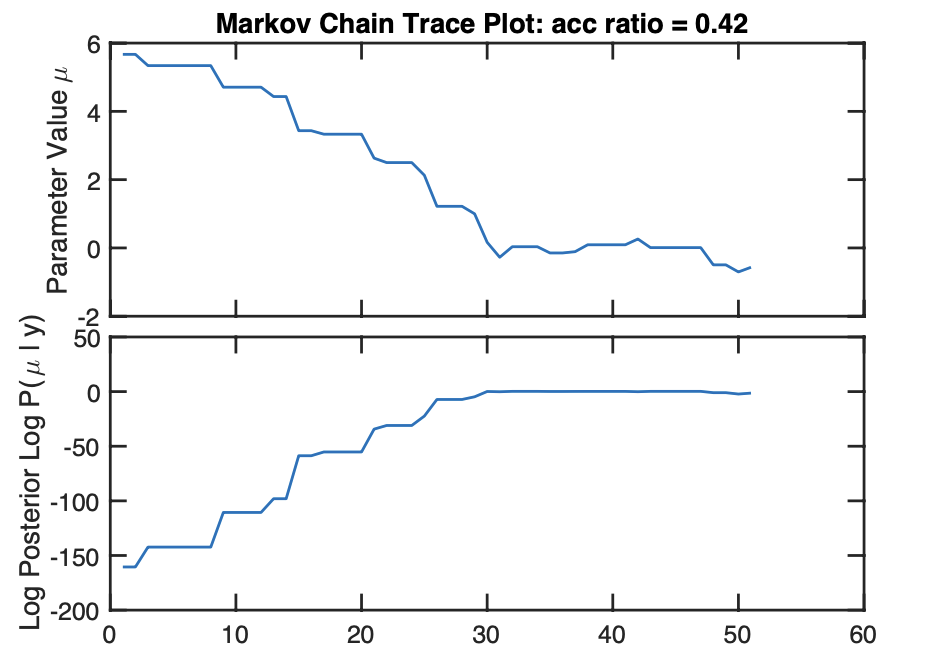
\includegraphics[width=0.5\linewidth]{MCMC_trace_plot.png}
    \caption{Trace plot for first 50 iterations}
    \label{fig:MCMC_trace_plot}
\end{figure}

\end{example*}
Here, acc ratio = 0.42 means that 42\% of the proposals are accepted. Although a trace plot alone does not prove convergence, it is a useful first check.


\subsubsection*{Burn-in and thinning}

In practical MCMC use, one often discards an initial portion of the chain, called the \textit{burn-in}, to reduce sensitivity to the starting point. One may also keep only every $k$th draw, called \textit{thinning}, in order to reduce autocorrelation and storage. For example, after running a chain for 2000 iterations, one may discard the first $50\%$ as burn-in and then thin by keeping every second sample. The retained draws are then used to form posterior histograms or compute posterior summaries.

\subsection{Multivariate Metropolis algorithm: symmetric proposal distribution}

Now suppose the parameter is $\theta\in\mathbb{R}^d$. A symmetric proposal distribution is such that
\begin{equation*}
J(\theta^*\mid\theta)=J(\theta\mid\theta^*).
\end{equation*}

The \(d\)-dimensional Metropolis algorithm uses a multivariate Gaussian proposal:
\begin{equation*}
    \theta^* \sim J(\theta^*\mid\theta_{i-1})= \mathcal{N}(\theta\mid\theta_{i-1},\Sigma_p),
\end{equation*}
where $\Sigma_p$ is the proposal covariance matrix. 
Note that $J$ is indeed symmetric:
\begin{equation*}
    J(\theta\mid\theta^*)=|2\pi\Sigma_p|^{-\frac{1}{2}}\exp\left(-\frac{1}{2}(\theta-\theta^*)^T\Sigma_p^{-1}(\theta-\theta^*)\right)= J(\theta^*\mid\theta)
\end{equation*}
The algorithm is :
\begin{enumerate}
    \item choose a starting point $\theta_0$;
    \item propose $\theta^*\sim \mathcal{N}(\theta_{i-1},\Sigma_p)$;
    \item compute $r=P(\theta^*\mid y)/P(\theta_{i-1}\mid y)$;
    \item accept $\theta^*$ with probability $\min(r,1)$, otherwise stay at $\theta_{i-1}$;
    \item repeat.
\end{enumerate}


\subsubsection*{Drawing multivariate Gaussian proposal vectors: Cholesky decomposition}

To implement the multivariate Gaussian proposal
$\theta^* \sim \mathcal{N}(\theta_{i-1},\Sigma_p),$
we need a way to draw such random vectors. Since $\Sigma_p$ is a covariance matrix, it is
real, symmetric, and positive-definite. Then a \textit{Cholesky decomposition} exists:
\begin{equation*}
    \Sigma_p=LL^T,
\end{equation*}
where $L$ is lower triangular.

Now let
\begin{equation*}
    z=(z_1,\dots,z_d)^T,
    \qquad
    z_i \overset{\mathrm{iid}}{\sim} \mathcal{N}(0,1).
\end{equation*}
Define
\begin{equation*}
    \theta^*=\theta_{i-1}+Lz.
\end{equation*}
Then
\begin{equation*}
    \mathbb{E}[\theta^*]=\theta_{i-1},
\end{equation*}
and
\begin{align*}
    \mathrm{Cov}(\theta^*,\theta^{*T})
    = \mathrm{Cov}(Lz,(Lz)^T)= L\,\mathrm{Cov}(z,z^T)\,L^T= LIL^T= LL^T= \Sigma_p.
\end{align*}
$\theta^*$ is an affine transformation of Gaussian random variables, so it is also Gaussian. Thus, its distribution is specified by the mean and covariance:
\begin{equation*}
    \theta^*\sim \mathcal{N}(\theta_{i-1},\Sigma_p).
\end{equation*}



\subsection{Metropolis--Hastings algorithm: asymmetric proposal distribution}

The Metropolis algorithm assumes a symmetric proposal distribution. More generally, suppose the proposal density is
\begin{equation*}
    \theta^*\sim J(\theta^*\mid \theta_i),
\end{equation*}
where $J(a\mid b)$ need not equal $J(b\mid a)$. In practice, we can simply have $\theta^*\sim J(\theta^*)$, that is, the proposal distribution need not depend on $\theta_i$.
In this case, we use the \textit{Metropolis--Hastings algorithm}:
\begin{enumerate}
    \item choose a starting point $\theta_0$;
    \item propose $\theta^*\sim J(\theta^*\mid \theta_{i-1})$;
    \item compute
    \begin{equation*}
        r=
        \frac{P(\theta^*\mid y)\,J(\theta_{i-1}\mid \theta^*)}
             {P(\theta_{i-1}\mid y)\,J(\theta^*\mid \theta_{i-1})};
    \end{equation*}
    \item accept $\theta^*$ with probability $\min(r,1)$, otherwise stay at $\theta_{i-1}$;
    \item repeat.
\end{enumerate}

We can justify that Metropolis-Hasting respects detailed balance using similar argument as Metropolis algorithm.

\begin{remark}
    Note that the only difference is the ratio $r$. If $J$ is symmetric, then $r$ is the same as in Metropolis algorithm for symmetric proposal distribution. 
\end{remark}


\subsection{Gibbs sampling}

\subsubsection*{Gibbs sampling as a special case of Metropolis--Hastings}

Recall that the Metropolis--Hastings algorithm targets a posterior
$P(\theta\mid D)$ by proposing a move from the current state $\theta$ to a proposed state $\theta^*$ from a proposal distribution $J(\theta^*\mid \theta)$, then accepting with probability $\min(r,1)$, where
\begin{equation*}
    r
    =
    \frac{P(\theta^*\mid D)\,J(\theta\mid \theta^*)}
         {P(\theta\mid D)\,J(\theta^*\mid \theta)}.
\end{equation*}

\textit{Gibbs sampling} is a special case of Metropolis--Hastings for multidimensional sampling, when one can use the conditional posterior distributions themselves as proposal distributions. We will show that in this case, the Metropolis--Hastings ratio is equal to $1$, so proposals are always accepted. Also, since Gibbs sampling is a special case, detailed balance is automatically satisfied. 



\subsubsection*{Two-dimensional Gibbs sampler}

Suppose the posterior is $P(\theta,\phi\mid D)$ and both conditional posteriors are tractable:
$P(\theta\mid \phi,D)$ and $P(\phi\mid \theta,D)$.

A two-dimensional Gibbs sampler proceeds as follows:
\begin{enumerate}
    \item Choose a starting point $(\theta^0,\phi^0)$.
    \item At cycle $t$, update
    \begin{equation*}
        \theta^t \sim P(\theta\mid \phi^{t-1},D).
    \end{equation*}
    \item Then update
    \begin{equation*}
        \phi^t \sim P(\phi\mid \theta^t,D).
    \end{equation*}
    \item Record the current state $(\theta^t,\phi^t)$.
    \item Repeat until the chain appears to have converged and enough samples have been collected.
\end{enumerate}
Each complete pair of updates is called a \textit{Gibbs cycle}.

Note that in step 4, we implicitly set the Metropolis-Hasting ratio to be $r=1$. For example, when updating $\theta$ with $\phi$ fixed, we propose
\begin{equation*}
    \theta^* \sim P(\theta^*\mid \phi^{t-1},D).
\end{equation*}
Then the Metropolis--Hastings ratio is
\begin{equation*}
    r=
    \frac{P(\theta^*,\phi^{t-1}\mid D)\,P(\theta^{t-1}\mid \phi^{t-1},D)}
         {P(\theta^{t-1},\phi^{t-1}\mid D)\,P(\theta^*\mid \phi^{t-1},D)}
    =\frac{P(\phi^{t-1}\mid D)}{P(\phi^{t-1}\mid D)}
    =1,
\end{equation*}
because $P(\theta,\phi\mid D)=P(\theta\mid \phi,D)P(\phi\mid D)$. Hence Gibbs proposals are always accepted.

\subsubsection*{d-dimensional Gibbs sampler}

More generally, let $\vec{\theta}=(\theta_1,\dots,\theta_d)$. A Gibbs sampler updates the parameters one at a time within each cycle. At iteration cycle $t$, define the intermediate state before updating the $j$th coordinate by
\begin{equation*}
\vec{\theta}^{(t,j-1)}
:=
\bigl(
\theta_1^{(t)},\dots,\theta_{j-1}^{(t)},\theta_j^{(t-1)},\theta_{j+1}^{(t-1)},\dots,\theta_d^{(t-1)}
\bigr),
\end{equation*}
for $j=1,\dots,d$, with $\vec{\theta}^{(t,0)}:=\vec{\theta}^{(t-1)}$.

We also define
\begin{equation*}
\vec{\theta}_{-j}^{(t,j-1)}
:=
\bigl(
\theta_1^{(t)},\dots,\theta_{j-1}^{(t)},\theta_{j+1}^{(t-1)},\dots,\theta_d^{(t-1)}
\bigr),
\end{equation*}
that is, the current components of $\vec{\theta}$ except $\theta_j$, using the already updated values up to coordinate $j-1$.

We use the conditional posterior distribution for the Gibbs update for the $j$th component:
\begin{equation*}
\theta_j^{(t)} \sim P\bigl(\theta_j \mid \vec{\theta}_{-j}^{(t,j-1)}, D\bigr).
\end{equation*}

Equivalently, the proposal distribution at the $j$th substep only updates the $j$th component of $\vec{\theta}^{(t,j-1)}$, so we can write the proposal distribution as
\begin{equation*}
J\bigl(\vec{\theta}^{\,*} \mid \vec{\theta}^{(t,j-1)}\bigr)
=
P\bigl(\theta_j^* \mid \vec{\theta}_{-j}^{(t,j-1)}, D\bigr)
\,\mathbf{1}\bigl\{\vec{\theta}_{-j}^{\,*}=\vec{\theta}_{-j}^{(t,j-1)}\bigr\}.
\end{equation*}

Note that the indicator makes sure that $J$ only updates the $j$th component of $\vec{\theta}^{(t,j-1)}$. Now, by construction of $J$, we have
\begin{align*}
J\bigl(\vec{\theta}^{(t,j-1)} \mid \vec{\theta}^{\,*}\bigr)
&=
P\bigl(\theta_j^{(t-1)} \mid \vec{\theta}_{-j}^{\,*}, D\bigr)
\,\mathbf{1}\bigl\{\vec{\theta}_{-j}^{(t,j-1)}=\vec{\theta}_{-j}^{\,*}\bigr\} \\
&=
P\bigl(\theta_j^{(t-1)} \mid \vec{\theta}_{-j}^{(t,j-1)}, D\bigr)
\,\mathbf{1}\bigl\{\vec{\theta}_{-j}^{\,*}=\vec{\theta}_{-j}^{(t,j-1)}\bigr\}.
\end{align*}

Substituting this proposal into the Metropolis--Hastings ratio gives
\begin{align*}
r
&=
\frac{
P(\vec{\theta}^{\,*} \mid D)\,
J\bigl(\vec{\theta}^{(t,j-1)} \mid \vec{\theta}^{\,*}\bigr)
}{
P\bigl(\vec{\theta}^{(t,j-1)} \mid D\bigr)\,
J\bigl(\vec{\theta}^{\,*} \mid \vec{\theta}^{(t,j-1)}\bigr)
} \\
&=
\frac{
P\bigl(\theta_j^*,\vec{\theta}_{-j}^{(t,j-1)} \mid D\bigr)\,
P\bigl(\theta_j^{(t-1)} \mid \vec{\theta}_{-j}^{(t,j-1)}, D\bigr)
}{
P\bigl(\theta_j^{(t-1)},\vec{\theta}_{-j}^{(t,j-1)} \mid D\bigr)\,
P\bigl(\theta_j^* \mid \vec{\theta}_{-j}^{(t,j-1)}, D\bigr)
} \\
&=
\frac{
P\bigl(\theta_j^* \mid \vec{\theta}_{-j}^{(t,j-1)}, D\bigr)\,
P\bigl(\vec{\theta}_{-j}^{(t,j-1)} \mid D\bigr)\,
P\bigl(\theta_j^{(t-1)} \mid \vec{\theta}_{-j}^{(t,j-1)}, D\bigr)
}{
P\bigl(\theta_j^{(t-1)} \mid \vec{\theta}_{-j}^{(t,j-1)}, D\bigr)\,
P\bigl(\vec{\theta}_{-j}^{(t,j-1)} \mid D\bigr)\,
P\bigl(\theta_j^* \mid \vec{\theta}_{-j}^{(t,j-1)}, D\bigr)
} \\
&= 1.
\end{align*}

Hence each Gibbs update is always accepted. After updating all coordinates $j=1,\dots,d$, we set
\begin{equation*}
\vec{\theta}^{(t)}:=\vec{\theta}^{(t,d)}.
\end{equation*}


\subsection{Metropolis-within-Gibbs}

Gibbs sampling requires that each conditional posterior
$P(\theta_j\mid \theta_{-j},D)$
be tractable, meaning that we can draw from it directly. In many realistic models this is not possible for all coordinates.

We use \textit{Metropolis-within-Gibbs}: for each parameter whose conditional posterior is not directly sampleable, replace that Gibbs substep by a one-dimensional Metropolis update conditional on the current values of the other parameters.

Thus a mixed Gibbs sampler may:
\begin{itemize}
    \item sample exactly from tractable conditional posteriors for some parameters;
    \item use accept/reject Metropolis updates for the remaining parameters.
\end{itemize}

\subsubsection*{d-dimensional Metropolis-within-Gibbs sampler}

Let $\theta=(\theta_1,\dots,\theta_d)$ and define
\begin{equation*}
    \theta_{-j}^t
    :=
    (\theta_1^{t+1},\dots,\theta_{j-1}^{t+1},\theta_{j+1}^t,\dots,\theta_d^t).
\end{equation*}
At cycle $t=1,\dots,N$, cycle through the coordinates $j=1,\dots,d$:

\begin{enumerate}
    \item Propose a new value for the $j$th coordinate from a one-dimensional Gaussian:
    \begin{equation*}
        \theta_j^* \sim \mathcal{N}(\theta_j^t,\tau_j^2).
    \end{equation*}
    \item Compute the Metropolis ratio
    \begin{equation*}
        r
        =
        \frac{P(\theta_j^*,\theta_{-j}^t\mid D)}
             {P(\theta_j^t,\theta_{-j}^t\mid D)}
        =
        \frac{P(\theta_j^*\mid \theta_{-j}^t,D)}
             {P(\theta_j^t\mid \theta_{-j}^t,D)}.
    \end{equation*}
    \item Accept $\theta_j^{t+1}=\theta_j^*$ with probability $\min(r,1)$, otherwise, $\theta_j^{t+1}=\theta_j^t$.
\end{enumerate}
After completing all $d$ substeps, record the updated state $\theta^{t+1}$.

\subsection{Tuning Metropolis proposals}



\subsubsection*{Laplace approximation}
For a \(d\)-dimensional Metropolis proposal
\begin{equation*}
    \theta^*\sim \mathcal{N}(\theta_i,\Sigma_p),
\end{equation*}
the choice of proposal covariance $\Sigma_p$ is crucial.

If $\Sigma_p$ is too large, proposed moves will be too large, so too many proposals are rejected and the chain hardly moves. If $\Sigma_p$ is too small, the chain accepts many tiny moves: inefficient random walk. So the proposal must be scaled carefully for efficient exploration of the posterior.

A useful guide for tuning comes from the \textit{Laplace approximation}. Let the unnormalised posterior be
\begin{equation*}
    \tilde P(\theta\mid D)=P(D\mid \theta)P(\theta).
\end{equation*}
Define the \textit{Maximum A Posteriori} (\textit{MAP}) estimate by
\begin{equation*}
    \theta_{\mathrm{MAP}}=\arg\max_\theta \ln \tilde P(\theta\mid D).
\end{equation*}
A second-order Taylor expansion of $\ln \tilde P(\theta\mid D)$ around $\theta_{\mathrm{MAP}}$ gives
\begin{equation*}
    \ln \tilde P(\theta\mid D)
    \approx
    \ln \tilde P(\theta_{\mathrm{MAP}}\mid D)
    -\frac{1}{2}(\theta-\theta_{\mathrm{MAP}})^T
    A(\theta-\theta_{\mathrm{MAP}}),
\end{equation*}
where
\begin{equation*}
    A_{ij}
    =
    -\left.\frac{\partial^2}{\partial \theta_i\partial \theta_j}
    \ln \tilde P(\theta\mid D)\right|_{\theta=\theta_{\mathrm{MAP}}}.
\end{equation*}
Note that the first order term vanishes because $\theta_{\mathrm{MAP}}$ is at the maximum of $\ln \tilde P(\theta\mid D)$.
Exponentiating gives the Gaussian approximation
\begin{equation*}
    P(\theta\mid D)\approx \tilde P(\theta_{\mathrm{MAP}}\mid D)\times \exp\left(-\frac{1}{2}(\theta-\theta_{\mathrm{MAP}})^TA(\theta-\theta_{\mathrm{MAP}})\right)
    \approx
    \mathcal{N}(\theta\mid \theta_{\mathrm{MAP}},A^{-1}).
\end{equation*}
Here, $A^{-1}$ is an approximate posterior covariance matrix.

In practice, we choose the proposal scale to be 
\begin{equation*}
    \Sigma_p=c^2A^{-1},
\end{equation*}
where
\begin{equation*}
    c\approx \frac{2.4}{\sqrt{\dim(\theta)}}.
\end{equation*}
This scale aim for an acceptance ratio of 44\% in 1D, and 23\% in dimension$>5$.




\subsubsection*{Gelman--Rubin ratio}

Suppose we run $m$ parallel (\textit{i.e.} independent) chains of length $n$. Let $\psi_{ij}$ denote draw $i$ from chain $j$, and define the quantities
\begin{equation*}
    \bar\psi_{\cdot j}=\frac{1}{n}\sum_{i=1}^n \psi_{ij},
    \qquad
    \bar\psi_{\cdot\cdot}=\frac{1}{m}\sum_{j=1}^m \bar\psi_{\cdot j}, \qquad  s_j^2=\frac{1}{n-1}\sum_{i=1}^n (\psi_{ij}-\bar\psi_{\cdot j})^2.
\end{equation*}
The between-sequence and within-sequence variances are:
\begin{equation*}
    B=\frac{n}{m-1}\sum_{j=1}^m (\bar\psi_{\cdot j}-\bar\psi_{\cdot\cdot})^2, \qquad
    W=\frac{1}{m}\sum_{j=1}^m s_j^2.
\end{equation*}
An estimate of the marginal posterior variance is
\begin{equation*}
    \widehat{\mathrm{var}}^+(\psi\mid y)
    =
    \frac{n-1}{n}W+\frac{1}{n}B.
\end{equation*}
The Gelman--Rubin potential scale reduction factor is then
\begin{equation*}
    \hat R=\sqrt{\frac{\widehat{\mathrm{var}}^+(\psi\mid y)}{W}}.
\end{equation*}
A value
\begin{equation*}
    \hat R\approx 1
\end{equation*}
indicates that between-sequance and within-sequence variances are similar, which is evidence for convergence.



\subsubsection*{Autocorrelation and effective sample size}
Let a scalar chain be $(\theta_1,\dots,\theta_N)$. Consider the sample mean
\begin{equation*}
    \bar\theta=\frac{1}{N}\sum_{i=1}^N \theta_i.
\end{equation*}
If the chain were serially uncorrelated, that is $\mathrm{Cov}(\theta_i,\theta_j)=0$ for all $i\ne j$,
then
\begin{equation*}
    \mathrm{Var}(\bar\theta)=\frac{\mathrm{Var}(\theta)}{N}.
\end{equation*}
However, an MCMC chain is typically serially correlated:
\begin{equation*}
    \mathrm{Cov}(\theta_i,\theta_j)=C_{|i-j|}=\mathrm{Var}(\theta)\rho_{|i-j|},
\end{equation*}
where $\rho_t$ is the lag-$t$ autocorrelation.

For large $N$,
\begin{align*}
    \mathrm{Var}(\bar\theta)
    &=\frac{1}{N^2}\sum_{i=1}^N\sum_{j=1}^N\mathrm{Cov(\theta_i,\theta_j)}\\
    &=\frac{1}{N^2}\sum_{i=1}^N\sum_{j=1}^N\mathrm{Var(\theta)}\rho_{|i-j|}\\
    &=\frac{\mathrm{Var}(\theta)}{N^2}\left(N\rho_0+2(N-1)\rho_1+\cdots+2\cdot 1\cdot\rho_{N-1}\right)\\
    &=\frac{\mathrm{Var}(\theta)}{N}\left(1+2\sum_{t=1}^{N-1}\left(1-\frac{t}{N}\right)\rho_t\right)\\
    &\to \frac{\mathrm{Var}(\theta)\,\tau}{N}, \qquad \text{as $N\to\infty$},
\end{align*}
where
\begin{equation*}
    \tau=1+2\sum_{t=1}^\infty \rho_t
\end{equation*}
is the autocorrelation timescale. Equivalently,
\begin{equation*}
    \mathrm{Var}(\bar\theta)=\frac{\mathrm{Var}(\theta)}{N_{\mathrm{eff}}},
    \qquad
    N_{\mathrm{eff}}=\frac{N}{\tau}.
\end{equation*}
Here $N_{\mathrm{eff}}$ is the \textit{effective sample size}, which can be interpreted as the equivalent number of independent samples. Compare with the case that the $\theta_i$ are independent, where we got the formula
\begin{equation*}
     \mathrm{Var}(\bar\theta)=\frac{\mathrm{Var}(\theta)}{N},
\end{equation*}
so we can interpret $\tau$ as the number of iterations we need to get an independent sample. Also, $\tau$ indicates how efficient is the MCMC algorithm.

\subsubsection*{Estimating the autocorrelation/ESS}

For a scalar chain, the sample covariance of lag $t$ is
\begin{equation*}
    \hat C_t
    =
    \frac{1}{N-t-1}\sum_{i=1}^{N-t}(\theta_i-\bar\theta)(\theta_{i+t}-\bar\theta),
\end{equation*}
and the sample autocorrelation is
\begin{equation*}
    \hat\rho_t=\frac{\hat C_t}{\hat C_0},
\end{equation*}
where $\hat C_0$ is the sample variance of $\theta$.
Truncating at lag $T$, one estimates
\begin{equation*}
    \hat\tau=1+2\sum_{t=1}^T \hat\rho_t,
\end{equation*}
where $T$ is chosen large enough that $\hat\rho_T$ is close to zero, for example around $0.1$.
Then
\begin{equation*}
    N_{\mathrm{eff}}=\frac{N}{\hat\tau}
\end{equation*}
is the effective number of independent samples.



\subsection{Mixed Gibbs Samplers}

Suppose the target posterior is
\begin{equation*}
    \pi(\alpha,\beta,\theta),
\end{equation*}
and suppose that
\begin{equation*}
    \pi(\alpha\mid \beta,\theta),
    \qquad
    \pi(\beta\mid \alpha,\theta),
    \qquad
    \pi(\alpha,\beta\mid\theta)
\end{equation*}
are tractable, but
\begin{equation*}
    \pi(\theta\mid \alpha,\beta)
\end{equation*}
is not tractable. 
\subsubsection*{Mixed sampler}
\begin{enumerate}
    \item sample
    \begin{equation*}
        \alpha^t \sim \pi(\alpha\mid \beta^{t-1},\theta^{t-1});
    \end{equation*}
    \item sample
    \begin{equation*}
        \beta^t \sim \pi(\beta\mid \alpha^t,\theta^{t-1});
    \end{equation*}
    \item update $\theta^t$ by a Metropolis proposal/accept/reject step.
\end{enumerate}

\subsubsection*{Mixed sampler with blocking}
\begin{enumerate}
    \item jointly sample
    \begin{equation*}
        (\alpha^t,\beta^t)\sim \pi(\alpha,\beta\mid \theta^{t-1});
    \end{equation*}
    \item update $\theta^t$ by a Metropolis step.
\end{enumerate}
Blocking is typically more efficient when the blocked parameters are strongly correlated, because it allows the sampler to move in directions that better match the posterior geometry.








\subsection{MCMC in practice}

The practical workflow of MCMC is as follows.

\begin{enumerate}
    \item Find the mode or modes of the posterior by optimisation, and possibly use a Laplace approximation to obtain a proposal covariance matrix.
    \item Start multiple parallel chains from dispersed starting points near the relevant high-posterior regions.
    \item Tune Metropolis proposals to achieve an acceptance rate roughly in the range $25\%$--$50\%$, depending on the dimension and proposal structure.
    \item Use a proposal covariance matrix that reflects the posterior shape.
    \item Inspect trace plots for obvious problems.
    \item Compute Gelman--Rubin ratios to compare within-chain and between-chain variances and assess burn-in.
    \item Compute autocorrelation timescales and effective sample sizes to check that enough effectively independent samples have been obtained.
    \item If diagnostics are satisfactory, discard burn-in, thin if necessary, combine chains, and compute posterior summaries.
\end{enumerate}

\section{Gaussian Processes}

A \textit{Gaussian process} (GP) is a collection of random variables $\{f(t)\}$, indexed by some input variable $t$ (for example time, space, or wavelength), such that any finite subset has a joint multivariate Gaussian distribution. That is, if we choose finitely many input points $t_1,\dots,t_N$ and define
\begin{equation*}
    f=
    \begin{pmatrix}
        f(t_1)\\
        \vdots\\
        f(t_N)
    \end{pmatrix},
\end{equation*}
then $f$ is multivariate Gaussian. Therefore it is completely determined by its mean vector and covariance matrix.

A Gaussian process with \textit{mean function} $m(t)$ and \textit{covariance function} or \textit{kernel} $k(t,t')$, where
\begin{equation*}
    m(t)=\mathbb{E}[f(t)],
    \qquad
    k(t,t')=\mathrm{Cov}(f(t),f(t')),
\end{equation*}
is denoted
\begin{equation*}
    f(t)\sim \mathcal{GP}(m(t),k(t,t')).
\end{equation*}
A GP is a probability distribution over functions.


\subsubsection*{Review: conditioning in a multivariate Gaussian}

Suppose
\begin{equation*}
    \begin{pmatrix}
        U\\
        V
    \end{pmatrix}
    \sim
    \mathcal{N}\!\left(
    \begin{pmatrix}
        U_0\\
        V_0
    \end{pmatrix},
    \begin{pmatrix}
        \Sigma_U & \Sigma_{UV}\\
        \Sigma_{VU} & \Sigma_V
    \end{pmatrix}
    \right).
\end{equation*}
Then the conditional distribution of $U$ given $V$ is Gaussian:
\begin{equation*}
    U\mid V
    \sim
    \mathcal{N}\!\bigl(\mathbb{E}[U\mid V],\,\mathrm{Var}(U\mid V)\bigr),
\end{equation*}
with
\begin{align*}
    \mathbb{E}[U\mid V]
    &=
    U_0+\Sigma_{UV}\Sigma_V^{-1}(V-V_0),\\
    \mathrm{Var}(U\mid V)
    &=
    \Sigma_U-\Sigma_{UV}\Sigma_V^{-1}\Sigma_{VU}.
\end{align*}
In particular, if $V$ is the set of observed data, $U$ is the set of unobserved parameters, the $P(U\mid V)$ is a posterior pdf. 

\subsubsection*{Gaussian process as a prior on functions}
Although a GP is formally an infinite-dimensional object, in practice we only ever evaluate it on a finite set of points $t=(t_1,\dots,t_N)^T$, with function values $f=(f(t_1),\dots,f(t_N))^T$.

Assume a constant prior mean function $m(t)=c$, where usually we have $c=0$,
so the mean vector is ${1}c$, where $1$ denotes the vector of ones.

A common kernel is the \textit{squared exponential kernel}
\begin{equation*}
    k(t,t')
    =
    A^2\exp\!\left(-\frac{|t-t'|^2}{\tau^2}\right),
\end{equation*}
where $A$ is an amplitude scale and $\tau$ is a characteristic length scale.

Then
\begin{equation*}
    f\mid A,\tau \sim \mathcal{N}(1c,K),
\end{equation*}
where the covariance matrix is defined by
\begin{equation*}
    K_{ij}=k(t_i,t_j)=A^2\exp\!\left(-\frac{|t_i-t_j|^2}{\tau^2}\right).
\end{equation*}


\subsubsection*{Fitting a GP to data}

There are two distinct problems.

\begin{enumerate}
    \item \textit{Prediction}: If we knew the characteristic scales of
    the kernel (hyperparameters) $(A,\tau^2)$, then how do we  fit the data at observed times to find the curve for unobserved times? (posterior predictive)
    \item \textit{Model selection}: Given the observed data, how do we fit for the characteristic scales of the kernel hyperparameters $(A,\tau)$?
\end{enumerate}


\subsection{Posterior inference with GP}

Suppose the function is observed exactly at a set of \textit{observed} input points $t_o$, with function values $f_o$, and we wish to predict the function at \textit{unobserved} points $t_*$, with latent values $f_*$.

Under the GP prior, the joint distribution is
\begin{equation*}
    \begin{pmatrix}
        f_o\\
        f_*
    \end{pmatrix}
    \sim
    \mathcal{N}\!\left(
    \begin{pmatrix}
        1c\\
        1c
    \end{pmatrix},
    \begin{pmatrix}
        K(t_o,t_o) & K(t_o,t_*)\\
        K(t_*,t_o) & K(t_*,t_*)
    \end{pmatrix}
    \right).
\end{equation*}
Applying the conditional Gaussian formula gives
\begin{equation*}
    f_*\mid f_o \sim \mathcal{N}\!\bigl(\mathbb{E}[f_*\mid f_o],\,\mathrm{Var}(f_*\mid f_o)\bigr),
\end{equation*}
where
\begin{align*}
    \mathbb{E}[f_*\mid f_o]
    &=
    1c+K(t_*,t_o)K(t_o,t_o)^{-1}(f_o-1c),\\
    \mathrm{Var}(f_*\mid f_o)
    &=
    K(t_*,t_*)-K(t_*,t_o)K(t_o,t_o)^{-1}K(t_o,t_*).
\end{align*}
This is the \textit{posterior predictive distribution} for the function.

\subsubsection*{Accounting for measurement error}

In practice, we cannot ignore observation errors. 
To account for noisy observations, let $y_o$
denote the observed values of the function at inputs $t_o$, and let $f_o$
denote the corresponding exact function values.

Assume the measurement model
\begin{equation*}
    y_o\mid f_o \sim \mathcal{N}(f_o,W),
\end{equation*}
where $W$ is the measurement-error covariance matrix. Equivalently,
\begin{equation*}
    y_o=f_o+\varepsilon,
    \qquad
    \varepsilon\sim \mathcal{N}(0,W).
\end{equation*}

The most common case is heteroskedastic uncorrelated measurement error:
\begin{equation*}
    \mathrm{Cov}(\varepsilon_i,\varepsilon_j)=W_{ij}=\delta_{ij}\sigma_i^2.
\end{equation*}

Assume $f$ and $\varepsilon$ are independent, then
\begin{align*}
    \mathrm{Cov}(y_o,y_o)
    &=
    \mathrm{Cov}(f_o+\varepsilon,\;f_o+\varepsilon)\\
    &=
    \mathrm{Cov}(f_o,f_o)+\mathrm{Cov}(\varepsilon,\varepsilon)
    +2\,\mathrm{Cov}(f_o,\varepsilon)\\
    &=
    K(t_o,t_o)+W.
\end{align*}
Similarly,
\begin{align*}
    \mathrm{Cov}(y_o,f_*)
    &=
    \mathrm{Cov}(f_o+\varepsilon,f_*)\\
    &=
    \mathrm{Cov}(f_o,f_*)+\mathrm{Cov}(\varepsilon,f_*)\\
    &=
    K(t_o,t_*),
\end{align*}
and of course
\begin{equation*}
    \mathrm{Cov}(f_*,f_*)=K(t_*,t_*).
\end{equation*}

Therefore the joint distribution of observed noisy data and function values at unobserved prediction points is
\begin{equation*}
    \begin{pmatrix}
        y_o\\
        f_*
    \end{pmatrix}
    \sim
    \mathcal{N}\!\left(
    \begin{pmatrix}
        1c\\
        1c
    \end{pmatrix},
    \begin{pmatrix}
        K(t_o,t_o)+W & K(t_o,t_*)\\
        K(t_*,t_o) & K(t_*,t_*)
    \end{pmatrix}
    \right).
\end{equation*}

\subsubsection*{Posterior predictive with measurement error}

Conditioning on the noisy observations $y_o$ now gives
\begin{equation*}
    f_*\mid y_o \sim \mathcal{N}\!\bigl(\mathbb{E}[f_*\mid y_o],\,\mathrm{Var}(f_*\mid y_o)\bigr),
\end{equation*}
with
\begin{align*}
    \mathbb{E}[f_*\mid y_o]
    &=
    1c+K(t_*,t_o)\bigl[K(t_o,t_o)+W\bigr]^{-1}(y_o-1c),\\
    \mathrm{Var}(f_*\mid y_o)
    &=
    K(t_*,t_*)-K(t_*,t_o)\bigl[K(t_o,t_o)+W\bigr]^{-1}K(t_o,t_*).
\end{align*}


\subsection{Tuning the hyperparameters}

\subsubsection*{Marginal likelihood}

Since
\begin{equation*}
    y_o\mid f_o \sim \mathcal{N}(f_o,W),
    \qquad
    f_o\mid A,\tau \sim \mathcal{N}\!\bigl(1c,\;K_{A,\tau}(t_o,t_o)\bigr),
\end{equation*}
equivalently,
\begin{equation*}
    f_o=1c+\varepsilon_{GP}, \qquad\varepsilon_{GP}\sim\mathcal{N}\!\bigl(0,\;K_{A,\tau}(t_o,t_o)\bigr),
\end{equation*}
and
\begin{equation*}
    y_o=f_o+\varepsilon_o,
    \qquad \varepsilon_o\sim \mathcal{N}(0,W),
\end{equation*}
so $y_o=1c+\varepsilon_{GP}+\varepsilon_o$.
Since the sum of independent Gaussian vectors is Gaussian, we have
\begin{equation*}
    P(y_o\mid A,\tau)
    =
    \mathcal{N}\!\bigl(y_o\mid 1c,\;K_{A,\tau}(t_o,t_o)+W\bigr).
\end{equation*}
This is the \textit{marginal likelihood} for the hyperparameters.

\subsubsection*{Maximum marginal likelihood}

One approach is to choose $(A,\tau)$ by maximizing the marginal likelihood:
\begin{equation*}
    (\hat A,\hat\tau)
    =
    \arg\max_{A,\tau} P(y_o\mid A,\tau).
\end{equation*}

\subsubsection*{Bayesian hyperparameter inference}

Instead of optimization, one may place a prior on $(A,\tau)$ and sample from the posterior
\begin{equation*}
    P(A,\tau\mid y_o)\propto P(y_o\mid A,\tau)\,P(A,\tau).
\end{equation*}


\subsection{Covariance functions}
A covariance function is
\begin{itemize}
    \item \textit{symmetric} if
    \begin{equation*}
        k(t,t')=k(t',t),
    \end{equation*}
    \item \textit{stationary} if 
    \begin{equation*}
        k(t,t')=k(t-t'),
    \end{equation*}
    i.e., it depends only on the difference between its arguments.
\end{itemize}


\subsubsection*{Squared exponential kernel}

The squared exponential kernel is
\begin{equation*}
    k(t,t')
    =
    A^2\exp\!\left(-\frac{|t-t'|^2}{\tau^2}\right).
\end{equation*}
Here $A$ is the characteristic amplitude and $\tau$ is the characteristic timescale.

This kernel gives very smooth sample curves: indeed, the corresponding GP sample functions are infinitely differentiable.


\subsubsection*{Exponential kernel and Ornstein--Uhlenbeck process}

Another important covariance function is the exponential kernel
\begin{equation*}
    k(t,t')
    =
    A^2\exp\!\left(-\frac{|t-t'|}{\tau}\right).
\end{equation*}
This is the covariance function of the \textit{Ornstein--Uhlenbeck process}, also called a \textit{damped random walk}. The associated stochastic differential equation is
\begin{equation*}
    df(t)=\tau^{-1}\bigl(\mu-f(t)\bigr)\,dt+\sigma\,dW_t,
\end{equation*}
where $W_t$ is the random walk, $\mu$ is the long-term mean, $\tau$ is the mean-reversion timescale, and $\sigma$ is the volatility. For this process, the stationary covariance takes the exponential form above.

\subsubsection*{Mat\'ern family}

The exponential kernel is a special case of the \textit{Mat\'ern} class. The Mat\'ern covariance function is
\begin{equation*}
    k_{\mathrm{Mat\acute ern}}(r)
    =
    \frac{2^{1-\nu}}{\Gamma(\nu)}
    \left(\frac{\sqrt{2\nu}\,r}{\ell}\right)^\nu
    K_\nu\!\left(\frac{\sqrt{2\nu}\,r}{\ell}\right),
\end{equation*}
where $r=|t-t'|$, $\nu>0$, $\ell>0$, and $K_\nu$ is the modified Bessel function.

When $\nu=p+\tfrac12$ is half-integer, the Mat\'ern kernel simplifies to an exponential times a polynomial. In particular, the case
    $\nu=\frac12$
gives exactly the exponential covariance function.

\subsubsection*{Periodic covariance functions}

Periodic covariance functions have kernel of the form
\begin{equation*}
    k(t,t')
    =
    A^2\exp\!\left(
    -\frac{2r^2}{\ell^2}\sin^2\!\left(\frac{\pi(t-t')}{T}\right)
    \right),
\end{equation*}
where $T$ is the period. This kernel produces functions that are periodic with period $T$, with smoothness controlled by $\ell$.

In general, the \textit{period} is defined by the number $P$ such that 
\begin{equation*}
    k(t+P,t') = k(t,t')\qquad\forall \, t,t'.
\end{equation*}

\section{Probabilistic graphical models}


A \textit{probabilistic graphical model} is a way to depict a complex probability distribution through a graph.

Let $a,b,c$ be random variables with joint pdf $P(a,b,c)$, which can be factorised as
\begin{equation*}
    P(a,b,c)=P(c\mid a,b)P(a,b)
    =P(c\mid a,b)P(b\mid a)P(a).
\end{equation*}
This factorisation can be represented by a \textit{directed acyclic graph} (\textit{DAG}) in which $a$ is a parent of $b$, and both $a$ and $b$ are parents of $c$.
\begin{figure}[H]
    \centering
    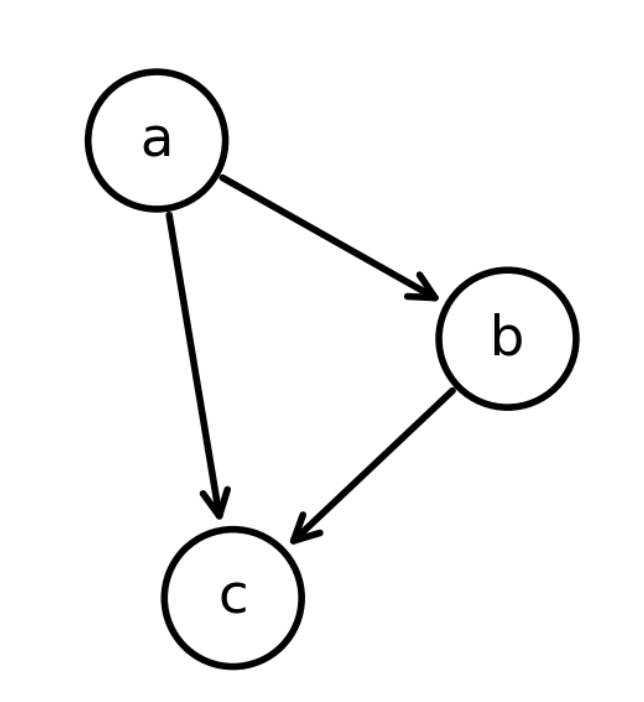
\includegraphics[width=0.2\linewidth]{DAG_Ex_3_Nodes.png}
    \label{fig:dag_3_nodes}
\end{figure}
More generally, let
\begin{equation*}
    \vec x=(x_1,\dots,x_K)
\end{equation*}
be a collection of random variables. Given a DAG, the joint distribution factorises as
\begin{equation*}
    P(\vec x)=\prod_{k=1}^K P\bigl(x_k\mid \mathrm{pa}(x_k)\bigr),
\end{equation*}
where $\mathrm{pa}(x_k)$ denotes the set of parents of $x_k$. If $x_k$ has no parents, then its factor is simply $P(x_k)$.

Consider the following DAG
\begin{figure}[H]
    \centering
    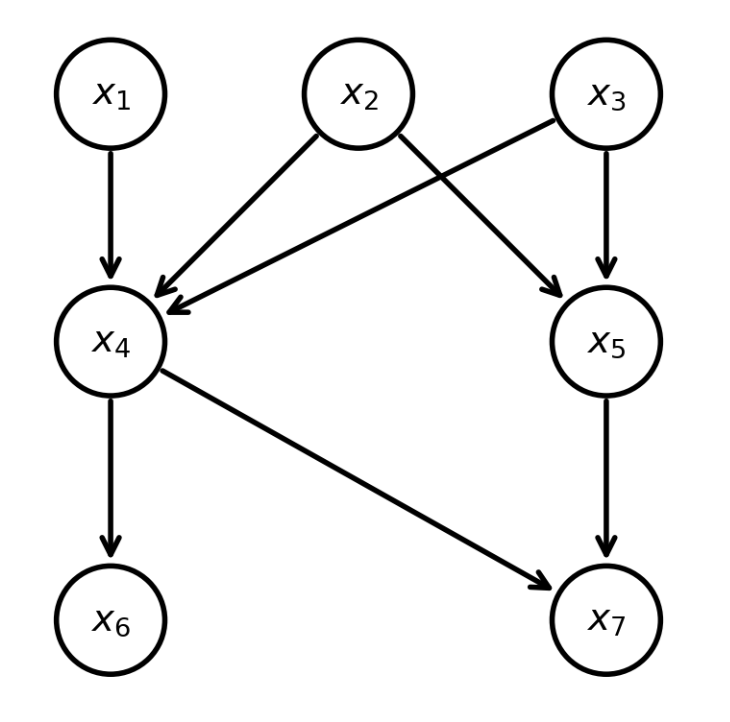
\includegraphics[width=0.2\linewidth]{DAG_Ex_7_Nodes.png}
    \label{fig:dag_7_nodes}
\end{figure}
Then the joint distribution factorises as
\begin{align*}
    P(x_1,\dots,x_7)
    &=
    P(x_1)P(x_2)P(x_3)
    P(x_4\mid x_1,x_2,x_3)
    P(x_5\mid x_2,x_3)
    P(x_6\mid x_4)
    P(x_7\mid x_4,x_5).
\end{align*}

\subsubsection*{Graphical notation}

The graphical notation is as follows.

An \textit{open node} denotes a latent parameter or unobserved datum.

A \textit{shaded node} denotes an observed parameter or observed datum, i.e. a variable that we condition on.

A \textit{filled dot} denotes a fixed and known constant.

A \textit{plate} denotes independent replication of the variables inside it.
\begin{figure}[H]
    \centering
    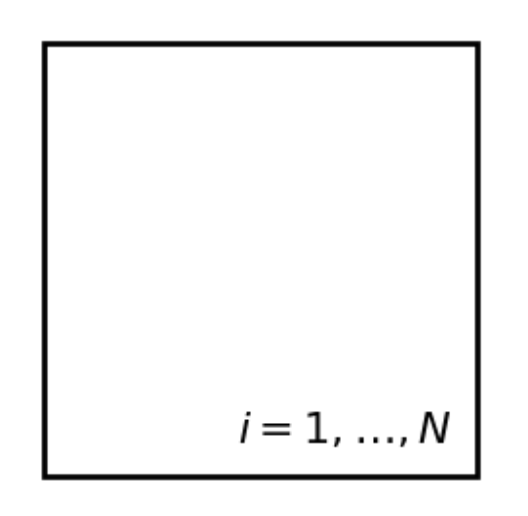
\includegraphics[width=0.2\linewidth]{DAG_Plate.png}
    \caption*{Plate}
    \label{fig:dag_plate}
\end{figure}

\begin{example*}
    Suppose
\begin{equation*}
    y_i \overset{\mathrm{iid}}{\sim} \mathcal{N}(\mu,\sigma^2=1),
    \qquad i=1,\dots,N.
\end{equation*}
Then the corresponding graphical model has $\mu$ as a parent of each $y_i$, with the known constant $\sigma^2=1$ also entering each observation model.
\begin{figure}[H]
    \centering
    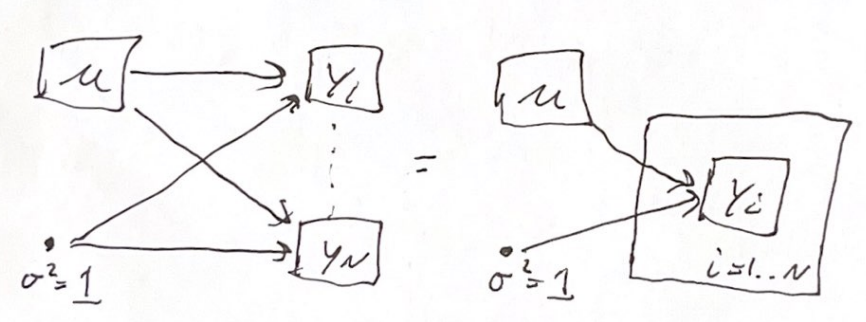
\includegraphics[width=0.5\linewidth]{DAG_Gaussian.png}
    \label{fig:placeholder}
\end{figure}

The joint distribution is
\begin{equation*}
    P(\mu,\vec y)
    =
    \left[\prod_{i=1}^N P(y_i\mid \mu)\right]P(\mu).
\end{equation*}
If the observations $\vec y=(y_1,\dots,y_N)$ are observed, then the posterior satisfies
\begin{equation*}
    P(\mu\mid \vec y)
    \propto
    \left[\prod_{i=1}^N P(y_i\mid \mu)\right]P(\mu).
\end{equation*}
\end{example*}


\subsection{Conditional independence}


Let $a,b,c$ be random variables.

We say that $a$ and $b$ are \textit{marginally independent} if
\begin{equation*}
    P(a,b)=P(a)P(b).
\end{equation*}
In this case we write
$$
a \perp b
\qquad \text{or} \qquad
a \perp b \mid \varnothing.
$$

We say that $a$ and $b$ are \textit{conditionally independent} given $c$ if
\begin{equation*}
    P(a,b\mid c)=P(a\mid c)P(b\mid c).
\end{equation*}
Equivalently,
\begin{equation*}
    P(a\mid b,c)=P(a\mid c).
\end{equation*}
In this case we write
$$
a \perp b \mid c.
$$

Conditional independence means that once $c$ is known, learning $b$ gives no extra information about $a$.

\begin{example*}[Common parent]
Suppose $ P(a,b,c)=P(c)P(a\mid c)P(b\mid c).$

\begin{figure}[H]
    \centering
    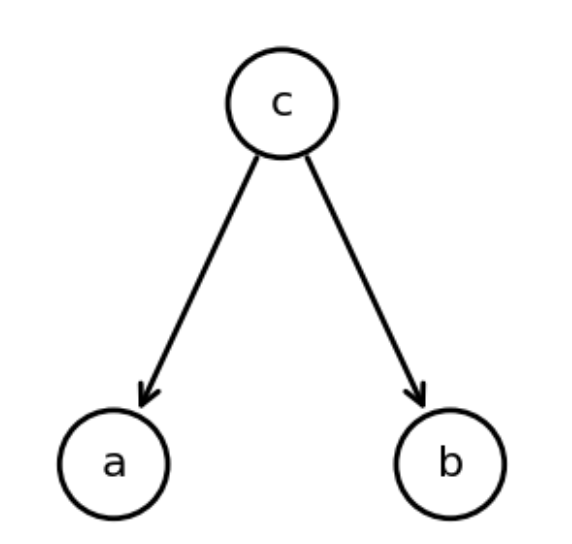
\includegraphics[width=0.2\linewidth]{c->a,b_unconditional.png}
\end{figure}
$ P(a,b)=\int P(c)P(a\mid c)P(b\mid c)\,dc\neq P(a)P(b),$ so $a \not\perp b.$ 

\begin{figure}[H]
    \centering
    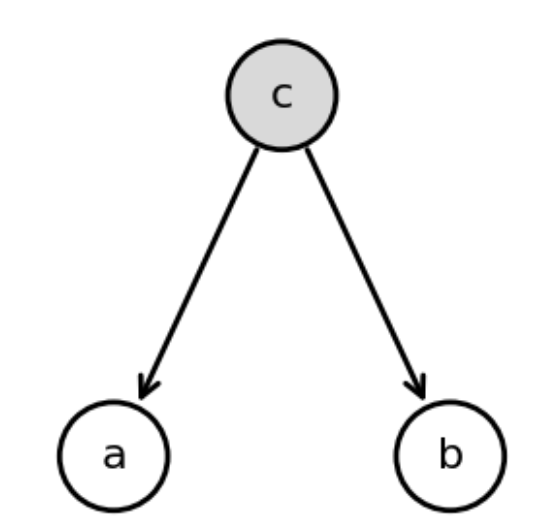
\includegraphics[width=0.2\linewidth]{c->a,b_conditional.png}
\end{figure}

$ P(a,b\mid c)=\frac{P(a,b,c)}{P(c)}=P(a\mid c)P(b\mid c),$ so
$a \perp b \mid c.$
\end{example*}

\begin{example*}[Collider]
Suppose $P(a,b,c)=P(a)P(b)P(c\mid a,b),$
\begin{figure}[H]
    \centering
    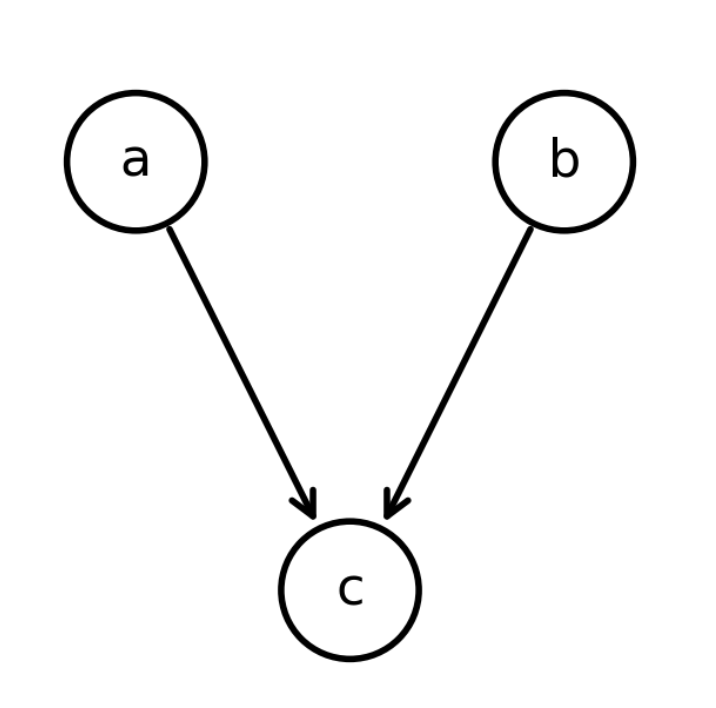
\includegraphics[width=0.2\linewidth]{a,b->c_unconditional.png}
\end{figure}
$ P(a,b)=P(a)P(b)\int P(c\mid a,b)\,dc=P(a)P(b),$ so $a \perp b.$
\begin{figure}[H]
    \centering
    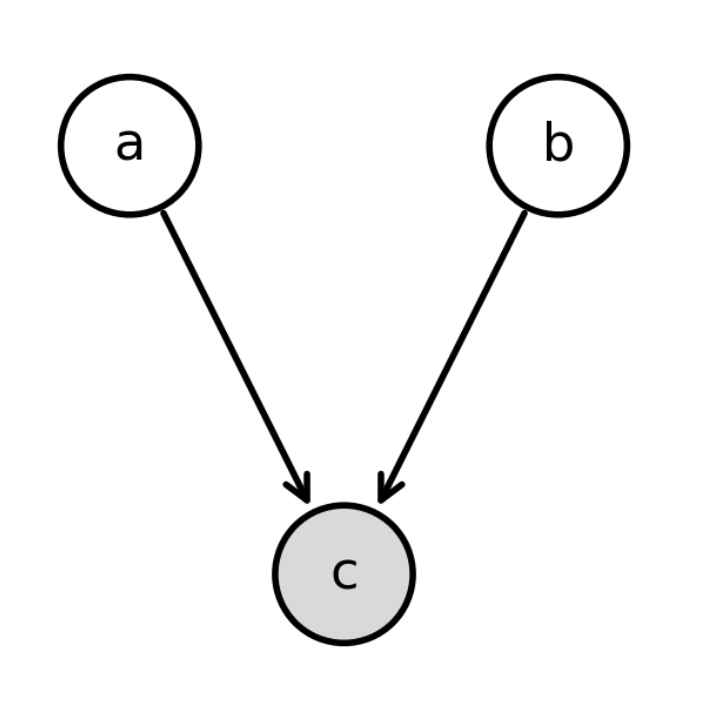
\includegraphics[width=0.2\linewidth]{a,b->c_conditional.png}
\end{figure}
$P(a,b\mid c)
    =
    \frac{P(a)P(b)P(c\mid a,b)}{P(c)}\neq P(a\mid c)P(b\mid c)$. Hence 
$
a \not\perp b \mid c.
$
\end{example*}


\subsection{Bayesian curve fitting}

\begin{figure}[H]
    \centering

    \begin{subfigure}{0.45\textwidth}
        \centering
        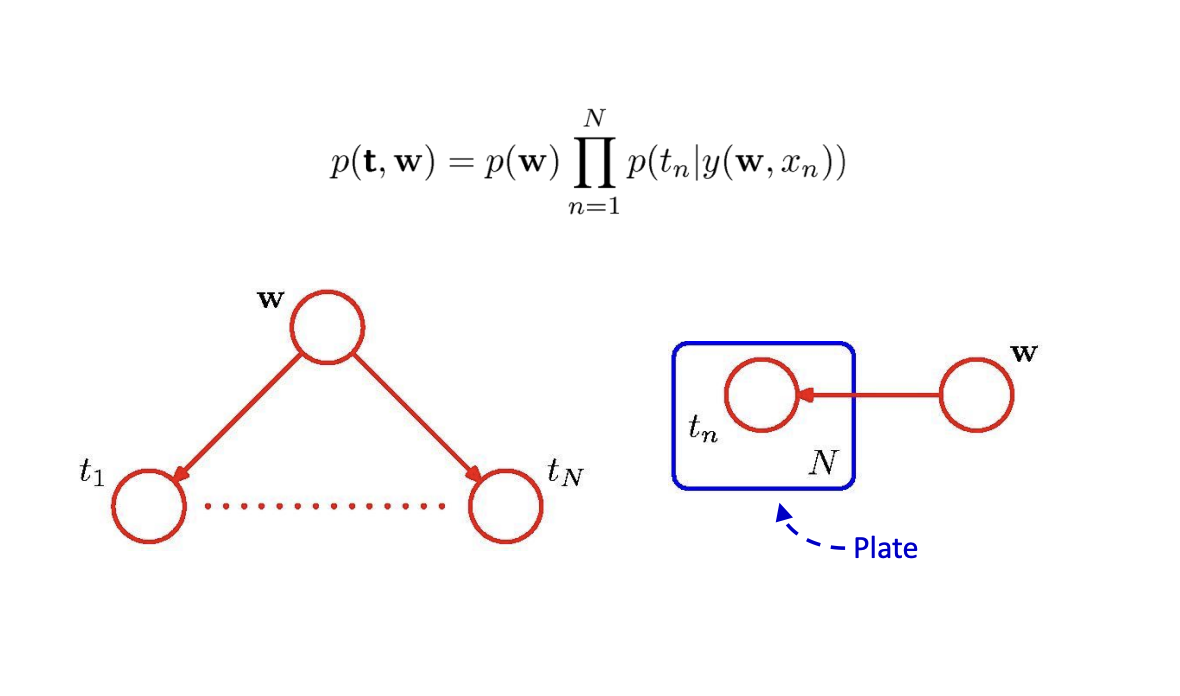
\includegraphics[width=\linewidth]{Bayesian_Fit_1.png}
    \end{subfigure}
    \hfill
    \begin{subfigure}{0.45\textwidth}
        \centering
        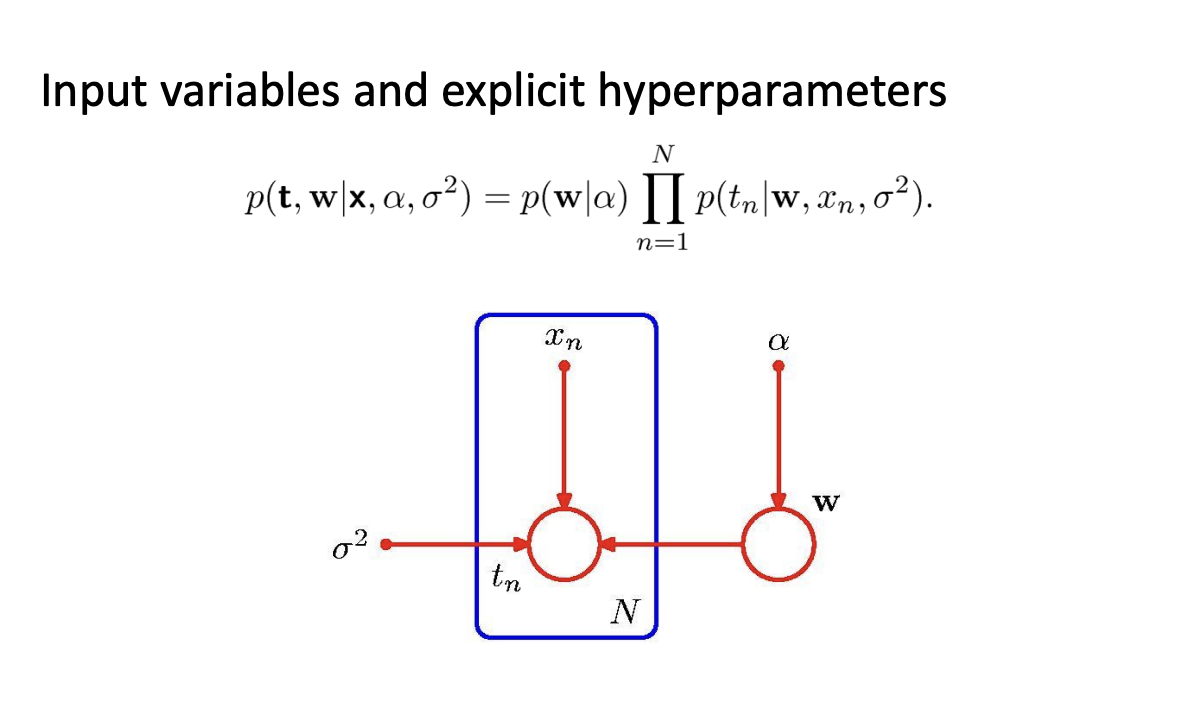
\includegraphics[width=\linewidth]{Bayesian_Fit_2.png}
    \end{subfigure}

    \vspace{0.5em}

    \begin{subfigure}{0.45\textwidth}
        \centering
        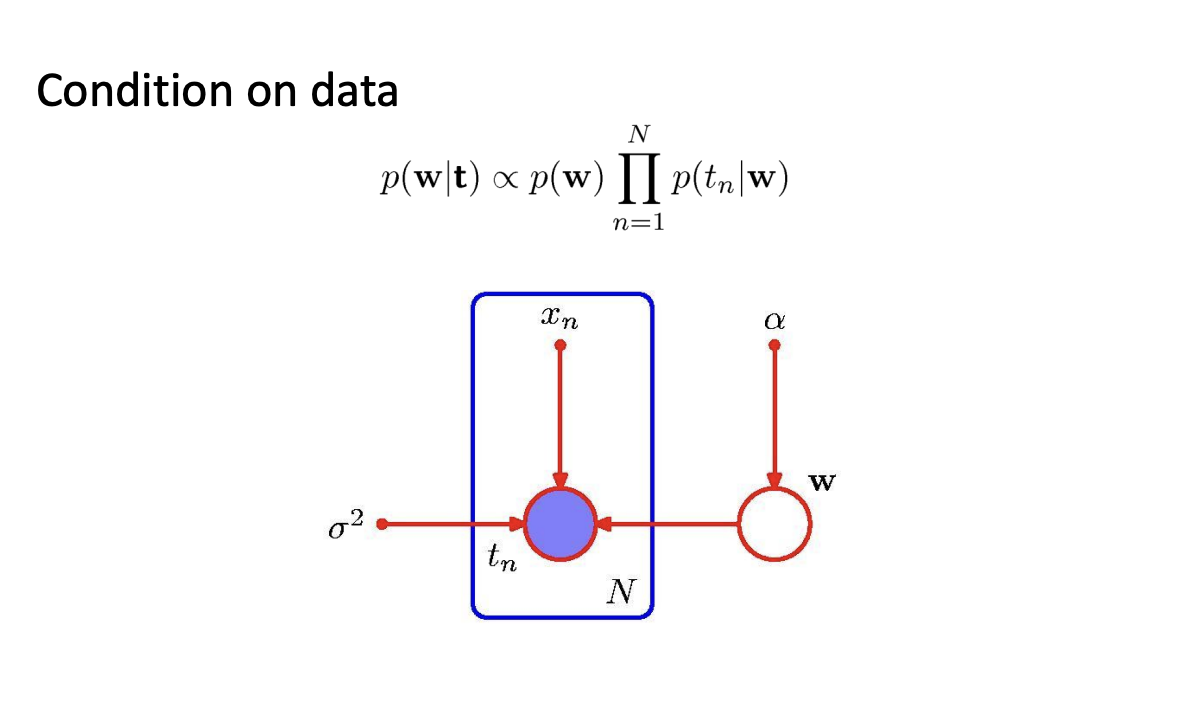
\includegraphics[width=\linewidth]{Bayesian_Fit_3.png}
    \end{subfigure}
    \hfill
    \begin{subfigure}{0.45\textwidth}
        \centering
        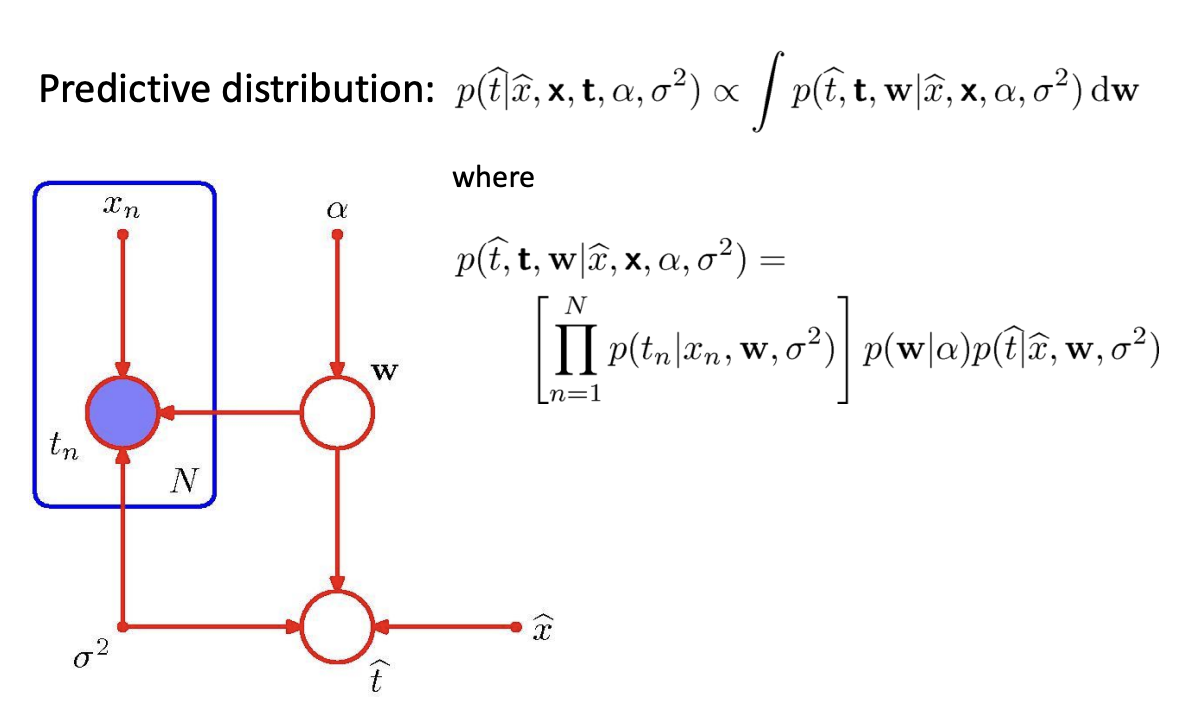
\includegraphics[width=\linewidth]{Bayesian_Fit_4.png}
    \end{subfigure}

    \label{fig:my_2by2}
\end{figure}

\subsection{D-separation}

\subsubsection*{Definition}

Let $A$, $B$, and $C$ be disjoint subsets of nodes in a DAG. A path from $A$ to $B$ is said to be blocked by $C$ if it contains a node such that either

\begin{enumerate}
    \item the arrows along the path meet head-to-tail or tail-to-tail at that node, and the node is in $C$; or
    \item the arrows meet head-to-head at that node, and neither the node nor any of its descendants are in $C$.
\end{enumerate}

If every path from $A$ to $B$ is blocked by $C$, then $A$ is said to be \textit{d-separated} from $B$ by $C$.

If $A$ is d-separated from $B$ by $C$, then the joint distribution over all variables in the graph satisfies
$
A \perp B \mid C.
$

\subsubsection*{Three basic local structures}

\paragraph{Fork:} \(a \leftarrow c \rightarrow b\)

Without conditioning on $c$, the variables $a$ and $b$ are generally dependent. Conditioning on $c$ blocks the path, so
$$
a \perp b \mid c.
$$

\paragraph{Chain:} \(a \rightarrow c \rightarrow b\)

Again, without conditioning on $c$, the variables $a$ and $b$ are generally dependent. Conditioning on $c$ blocks the path, so
$$
a \perp b \mid c.
$$

\paragraph{Collider:} \(a \rightarrow c \leftarrow b\)

Without conditioning on $c$, the path is blocked by $\emptyset$, so
$$
a \perp b.
$$
But once we condition on $c$, or on a descendant of $c$, the path becomes active, and typically
$$
a \not\perp b \mid c.
$$


\section{Hierarchical Bayes}


In simple Bayes, we have the likelihood $D\mid \theta \sim \mathrm{Model}(\theta),$
and the posterior is
\begin{equation*}
    P(\theta\mid D)\propto P(D\mid \theta)P(\theta).
\end{equation*}

In \textit{hierarchical Bayes}, we have
\begin{align*}
    D_i\mid \theta_i&\sim \mathrm{Model}(\theta_i),\\
    \theta_i\mid\alpha,\beta&\sim \mathrm{PopModel}(\alpha,\beta),
\end{align*}
where $\theta_i$ is the parameter of individual $i$, $\alpha,\beta$ are hyperparameters of the population. 
Then the joint posterior is
\begin{equation*}
    P(\{\theta_i\},\alpha,\beta\mid \{D_i\})
    \propto
    \left[\prod_{i=1}^N P(D_i\mid \theta_i)P(\theta_i\mid \alpha,\beta)\right]P(\alpha,\beta).
\end{equation*}
Hierarchical Bayes build up complexity by layering conditional probabilities. 


\subsection{The normal-normal model}
    Consider latent variables $M_1,\dots,M_N$ and observed data $D_1,\dots,D_N$ with known heteroskedastic measurement variances $\sigma_1^2,\dots,\sigma_N^2$.

At the population level, assume
\begin{equation*}
    M_s \sim \mathcal{N}(M_0,\tau^2),
    \qquad s=1,\dots,N,
\end{equation*}
where $M_0$ and $\tau^2$ are hyperparameters.

At the measurement level, assume
\begin{equation*}
    D_s\mid M_s \sim \mathcal{N}(M_s,\sigma_s^2),
    \qquad s=1,\dots,N.
\end{equation*}

The joint probability density of the data, latent variables, and hyperparameters is
\begin{equation*}
    P(\{D_s\},\{M_s\},M_0,\tau^2)
    =
    \left[\prod_{s=1}^N P(D_s\mid M_s)P(M_s\mid M_0,\tau^2)\right]P(M_0,\tau^2),
\end{equation*}
where $P(M_0,\tau^2)$ is the \textit{hyperprior}.

The posterior of all unknown quantities given the data is
\begin{equation*}
    P(\{M_s\},M_0,\tau^2\mid \{D_s\})
    \propto
    \left[\prod_{s=1}^N P(D_s\mid M_s)P(M_s\mid M_0,\tau^2)\right]P(M_0,\tau^2).
\end{equation*}

So the hierarchical model is just an ordinary Bayesian model on a larger parameter space, but its layered structure makes the modelling and computation much clearer.




\subsection{Gibbs sampling for the normal-normal model}
Consider the normal-normal model above, which reveals useful conditional independences.
\begin{enumerate}
    \item Each latent variable $M_s$ is conditionally independent of the other latent variables and of the other data. Hence
    \begin{equation*}
        P(M_s\mid M_0,\tau^2,\{D_r\}_{r=1}^N)
        =
        P(M_s\mid M_0,\tau^2,D_s).
    \end{equation*}
    \item Once the latent variables $\{M_s\}$ are known, the hyperparameters are conditionally independent of the observed data:
\begin{equation*}
    P(M_0,\tau^2\mid \{M_s\},\{D_s\})
    =
    P(M_0,\tau^2\mid \{M_s\}).
\end{equation*}
\end{enumerate}


\subsubsection*{Posterior for the latent variables}

For each $s=1,\dots,N$,
\begin{equation*}
    P(M_s\mid M_0,\tau^2,D_s)
    \propto
    P(D_s\mid M_s)P(M_s\mid M_0,\tau^2).
\end{equation*}
Since both factors are Gaussian, the conditional posterior of $M_s$ is Gaussian. By \cref{subsection:simple_gaussian_example}, we have
\begin{equation*}
    M_s\mid M_0,\tau^2,D_s
    \sim
    \mathcal{N}\!\left(
    \frac{D_s/\sigma_s^2 + M_0/\tau^2}{1/\sigma_s^2+1/\tau^2},
    \;
    \frac{1}{1/\sigma_s^2+1/\tau^2}
    \right).
\end{equation*}

\subsubsection*{Posterior for the hyperparemeters}

Assume the improper hyperprior
\begin{equation*}
    P(M_0,\tau^2)\propto 1.
\end{equation*}
Then
\begin{equation*}
    P(M_0,\tau^2\mid \{M_s\})
    =
    P(M_0\mid \tau^2,\{M_s\})P(\tau^2\mid \{M_s\}).
\end{equation*}
By \cref{subsection:multi-parameter_bayesian_inference:gaussian}, let
\begin{equation*}
    \bar M=\frac{1}{N}\sum_{s=1}^N M_s,
    \qquad
    s_M^2=\frac{1}{N-1}\sum_{s=1}^N (M_s-\bar M)^2.
\end{equation*}
Then
\begin{equation*}
    M_0\mid \tau^2,\{M_s\}
    \sim
    \mathcal{N}\!\left(\bar M,\frac{\tau^2}{N}\right),
\end{equation*}
and
\begin{equation*}
    \tau^2\mid \{M_s\}
    \sim
    \mathrm{Inv}\text{-}\chi^2\!\left(
    N-3,\;
    \frac{N-1}{N-3}s_M^2
    \right).
\end{equation*}

\subsubsection*{Gibbs sampling}

Since the posteriors are tractable, we can use Gibbs sampling. This is much more efficient than treating the problem as an undifferentiated Bayesian model in an $(N+2)$-dimensional parameter space and trying to update everything with a generic Metropolis sampler.



\subsection{Shrinkage in normal-normal model}
If one estimates each individual object separately, then the individual maximum likelihood estimator is simply 
$$\hat M_s=D_s.$$
This uses only the measurement model and ignores the population structure. In the hierarchical model, however, the posterior for each $M_s$ is based on both the data $D_s$ and the hyperparameters $M_0, \tau^2$ through
\begin{equation*}
    P(M_s\mid M_0,\tau^2,D_s)
    \propto
    P(D_s\mid M_s)P(M_s\mid M_0,\tau^2).
\end{equation*}

By above, we have
\begin{equation*}
    M_s\mid M_0,\tau^2,D_s
    \sim
    \mathcal{N}\!\left(
    \frac{D_s/\sigma_s^2 + M_0/\tau^2}{1/\sigma_s^2+1/\tau^2},
    \;
    \frac{1}{1/\sigma_s^2+1/\tau^2}
    \right).
\end{equation*}
So the posterior mean is
\begin{equation*}
    \mathbb{E}[M_s\mid M_0,\tau^2,D_s]
    =
    \frac{D_s/\sigma_s^2 + M_0/\tau^2}{1/\sigma_s^2+1/\tau^2}.
\end{equation*}
Therefore, unless $M_0=D_s$, the posterior mean lies between $M_0$ and $D_s$. In other words, the posterior estimate of $M_s$ is therefore pulled toward the population mean $M_0$. This is called \textit{shrinkage}.

Equivalently,
\begin{equation*}
    \mathbb{E}[M_s\mid M_0,\tau^2,D_s]
    =
    \lambda_s D_s + (1-\lambda_s)M_0,
\end{equation*}
where
\begin{equation*}
    \lambda_s=\frac{\tau^2}{\tau^2+\sigma_s^2}.
\end{equation*}
Thus, if $\tau^2$ is large, then $\lambda_s\approx 1$, so there is little shrinkage; if $\tau^2$ is small, then $\lambda_s$ is small, so the estimate is strongly pulled toward $M_0$. Also, the hyperparameter $\tau$ can be interpreted as the population width. Large population width means the latent variables may differ substantially, so weaker shrinkage is appropriate. On the other hand, small population width means the latent variables are believed to lie close together, so stronger shrinkage is appropriate. 



In a hierarchical Bayesian analysis, $\tau$ is itself unknown. Rather than fixing the amount of shrinkage by hand, the model infers it from the data through the posterior
\begin{equation*}
    P(\tau\mid D).
\end{equation*}


\section{Model selection}
Model selection is a higher level of inference than ordinary parameter estimation.

\subsection{Bayesian model comparison}

Let $M_1$ be a candidate model with parameter vector $\theta_1$. Its \textit{evidence}, or \textit{marginal likelihood}, is
\begin{equation*}
    P(D\mid M_1)=\int P(D\mid \theta_1,M_1)P(\theta_1\mid M_1)\,d\theta_1.
\end{equation*}

By Bayes' theorem, the posterior for the parameters within model $M_1$ is
\begin{equation*}
    P(\theta_1\mid D,M_1)
    =
    \frac{P(D\mid \theta_1,M_1)P(\theta_1\mid M_1)}{P(D\mid M_1)}.
\end{equation*}

The \textit{posterior odds ratio} between two models is
\begin{equation*}
    \frac{P(M_1\mid D)}{P(M_2\mid D)}
    =
    \frac{P(D\mid M_1)}{P(D\mid M_2)}
    \times
    \frac{P(M_1)}{P(M_2)},
\end{equation*}
where $P(M_1), P(M_2)$ are prior odds. 
The ratio
\begin{equation*}
    \mathrm{BF}_{12}
    =
    \frac{P(D\mid M_1)}{P(D\mid M_2)}
\end{equation*}
is the \textit{Bayes factor}.
\subsubsection*{Interpreting Bayes factors: the Jeffreys scale}

A Bayes factor is often interpreted through the logarithmic evidence difference
\begin{equation*}
    \Delta \ln E = \ln \mathrm{BF}.
\end{equation*}
The Jeffreys scale is
\begin{align*}
    &\Delta \ln E < 1 && \text{not worth more than a bare mention},\\
    &1 < \Delta \ln E < 2.5 && \text{ significant},\\
    &2.5 < \Delta \ln E < 5 && \text{strong to very strong},\\
    &5 < \Delta \ln E && \text{decisive}.
\end{align*}


\subsection{Occam's razor and the evidence}
The evidence is
\begin{equation*}
    p(D)=\int p(D\mid w)p(w)\,dw.
\end{equation*}
\begin{figure}[H]
    \centering
    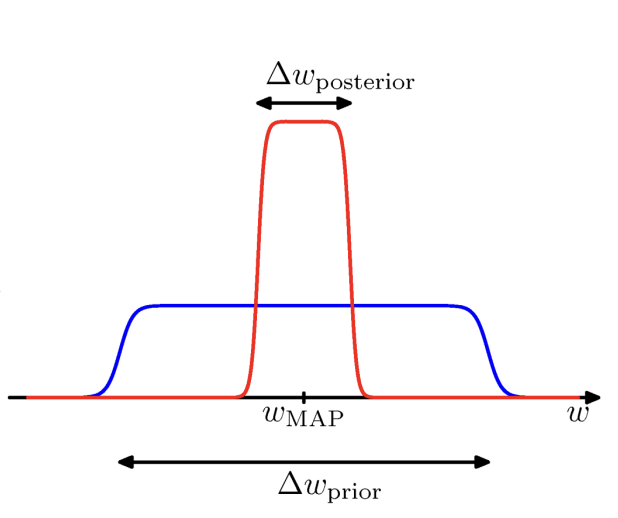
\includegraphics[width=0.5\linewidth]{Occam_Factor.png}
    \label{fig:occam_factor}
\end{figure}

If the posterior is sharply peaked around $w_{\mathrm{MAP}}$, where $w_{\mathrm{MAP}}$ is the maximizer of the posterior $P(D\mid w)$, then only a narrow region of width $\Delta w_{\mathrm{posterior}}$ contributes to the integral. If, in addition, the prior is approximately flat over width $\Delta w_{\mathrm{prior}}$, and approximately zero elsewhere, then
\begin{equation*}
    p(w)\approx \frac{1}{\Delta w_{\mathrm{prior}}},
\end{equation*}
and
\begin{equation*}
    p(D\mid w)\approx 
    p(D\mid w_{\mathrm{MAP}})
\end{equation*}
throughout the dominant region. Hence
\begin{equation*}
    p(D)\approx\int\frac{p(D\mid w_{\mathrm{MAP}})}{\Delta w_{\mathrm{prior}}}\, dw\approx p(D\mid w_{\mathrm{MAP}})
    \frac{\Delta w_{\mathrm{posterior}}}{\Delta w_{\mathrm{prior}}}.
\end{equation*}
Thus the evidence is approximately the best-fit likelihood multiplied by the \textit{Occam factor}
\begin{equation*}
     \frac{\Delta w_{\mathrm{posterior}}}{\Delta w_{\mathrm{prior}}}.
\end{equation*}




Taking logarithms,
\begin{equation*}
    \ln p(D)
    \approx
    \ln p(D\mid w_{\mathrm{MAP}})
    +
    \ln\!\left(\frac{\Delta w_{\mathrm{posterior}}}{\Delta w_{\mathrm{prior}}}\right).
\end{equation*}
Since typically $\Delta w_{\mathrm{posterior}} < \Delta w_{\mathrm{prior}}$, the second term is negative.


If the model has $M$ parameters, and each contributes a similar ratio of posterior width to prior width, then
\begin{equation*}
    \ln p(D)
    \approx
    \ln p(D\mid w_{\mathrm{MAP}})
    +
    M\ln\!\left(\frac{\Delta w_{\mathrm{posterior}}}{\Delta w_{\mathrm{prior}}}\right).
\end{equation*}
Thus, the log-evidence is negative linear in $M$, in other words, the model complexity $M$ is penalized linearly. 






\subsection{Laplace approximation to the evidence}

\subsubsection*{Laplace approximation to the posterior}

Let
\begin{equation*}
    P^*(\theta\mid D)=P(D\mid \theta)P(\theta)
\end{equation*}
denote the unnormalised posterior.

Let
\begin{equation*}
    \theta_0=\arg\max_\theta \ln P^*(\theta\mid D)
\end{equation*}
be the Maximum A Posteriori (MAP) estimate.

A second-order Taylor expansion around $\theta_0$ gives
\begin{equation*}
    \ln P^*(\theta\mid D)
    \approx
    \ln P^*(\theta_0\mid D)
    -\frac12(\theta-\theta_0)^T A(\theta-\theta_0),
\end{equation*}
where
\begin{equation*}
    A_{ij}
    =
    -\left.
    \frac{\partial^2}{\partial \theta_i \partial \theta_j}
    \ln P^*(\theta\mid D)
    \right|_{\theta=\theta_0}.
\end{equation*}
Exponentiating,
\begin{equation*}
    P^*(\theta\mid D)
    \approx
    P^*(\theta_0\mid D)
    \exp\!\left[
    -\frac12(\theta-\theta_0)^T A(\theta-\theta_0)
    \right].
\end{equation*}
Thus the posterior is approximated by a Gaussian with covariance matrix
\begin{equation*}
    \Sigma_{\mathrm{post}}=A^{-1}.
\end{equation*}

\subsubsection*{Evidence from the Laplace approximation}

The evidence is
\begin{equation*}
    P(D)=\int P^*(\theta\mid D)\,d\theta.
\end{equation*}
Using the Gaussian approximation,
\begin{align*}
    P(D)
    &\approx
    P^*(\theta_0\mid D)
    \int
    \exp\!\left[
    -\frac12(\theta-\theta_0)^T A(\theta-\theta_0)
    \right]d\theta\\
    &=
    P^*(\theta_0\mid D)\,|2\pi A^{-1}|^{1/2}.
\end{align*}
Since $P^*(\theta\mid D)=P(D\mid \theta)P(\theta)$ is the unnormalised posterior, we have
\begin{equation*}
    P(D)
    \approx
    P(D\mid \theta_0)P(\theta_0)\,\det(A/2\pi)^{-1/2}.
\end{equation*}

\subsubsection*{Occam factor in Gaussian form}

If the prior is Gaussian,
\begin{equation*}
    P(\theta)=\mathcal{N}(\theta\mid \theta_{\mathrm{prior}},\Sigma_{\mathrm{prior}}),
\end{equation*}
and the posterior covariance is
\begin{equation*}
    \Sigma_{\mathrm{post}}=A^{-1},
\end{equation*}
then the Occam factor satisfies
\begin{equation*}
     \frac{\Delta w_{\mathrm{posterior}}}{\Delta w_{\mathrm{prior}}}\propto\frac{|\Sigma_{\mathrm{post}}|^{1/2}}{|\Sigma_{\mathrm{prior}}|^{1/2}}.
\end{equation*}




\subsection{The harnomic mean estimator}

If $\theta_i\sim P(\theta)$ are sampled from the prior, then naive Monte Carlo gives
\begin{equation*}
    P(D)\approx \frac{1}{M}\sum_{i=1}^M P(D\mid \theta_i).
\end{equation*}
This is conceptually simple, but it is usually inefficient if the posterior occupies only a small fraction of the prior volume.

If $\theta_i\sim P(\theta\mid D)$ are sampled from the posterior, then the harmonic mean identity gives
\begin{equation*}
    P(D)\approx
    \left[
    \frac{1}{M}\sum_{i=1}^M P(D\mid \theta_i)^{-1}
    \right]^{-1}.
\end{equation*}
However, this estimator is often unstable.

\subsection{Savage--Dickey ratio}

Suppose the parameters are $\phi,\psi$ and the complex model $M_1$ is reduced to a simpler model $M_0$ when $\psi=0$ (nested).

Assume the prior for $M_1$ is separable
\begin{equation*}
    P(\phi,\psi\mid M_1)=P(\psi\mid M_1)P(\phi\mid M_1),
\end{equation*}
and the prior on $\phi$ is the same for each model
\begin{equation*}
    P(\phi\mid M_1)=P(\phi\mid M_0).
\end{equation*}

Under the full model $M_1$,
\begin{align*}
    P(\psi\mid D,M_1)
    &= \int P(\phi,\psi\mid D,M_1)\,d\phi\\
    &= \frac{1}{P(D\mid M_1)}
       \int P(D\mid \phi,\psi,M_1)P(\phi,\psi\mid M_1)\,d\phi.
\end{align*}
Using the separable prior
\begin{equation*}
    P(\phi,\psi\mid M_1)=P(\psi\mid M_1)P(\phi\mid M_1),
\end{equation*}
we obtain
\begin{equation*}
    P(\psi\mid D,M_1)
    =
    \frac{P(\psi\mid M_1)}{P(D\mid M_1)}
    \int P(D\mid \phi,\psi,M_1)P(\phi\mid M_1)\,d\phi.
\end{equation*}
Evaluating at $\psi=0$, and using the assumptions that $M_0$ is the submodel $\psi=0$ and that
\begin{equation*}
    P(\phi\mid M_1)=P(\phi\mid M_0),
\end{equation*}
gives
\begin{align*}
    P(\psi=0\mid D,M_1)
    &=
    \frac{P(\psi=0\mid M_1)}{P(D\mid M_1)}
    \int P(D\mid \phi,M_0)P(\phi\mid M_0)\,d\phi\\
    &=
    \frac{P(\psi=0\mid M_1)}{P(D\mid M_1)}P(D\mid M_0).
\end{align*}
Rearranging, the Bayes factor reduces to the Savage--Dickey ratio:
\begin{equation*}
    B_{01}
    =
    \frac{P(D\mid M_0)}{P(D\mid M_1)}
    =
    \left.
    \frac{P(\psi\mid D,M_1)}{P(\psi\mid M_1)}
    \right|_{\psi=0}.
\end{equation*}




\subsection{Bayesian model averaging}
\subsubsection*{Paremeter estimation}

If there are $N$ competing models $M_1,\dots,M_N$, then Bayes' theorem for each model gives
\begin{equation*}
    P(\theta\mid D,M_i)=\frac{P(D\mid \theta,M_i)P(\theta\mid M_i)}{P(D\mid M_i)}.
\end{equation*}

Then law of total probability gives the marginalised posterior over $N$ models. 
\begin{equation*}
    P(\theta\mid D)
    =
    \sum_{i=1}^N P(\theta\mid D,M_i)P(M_i\mid D).
\end{equation*}
\subsubsection*{Prediction of new data}

Similarly, for prediction of new data $\tilde D$, the posterior predictive under one model is
\begin{equation*}
    P(\tilde D\mid D,M_i)
    =
    \int P(\tilde D\mid \theta,M_i)P(\theta\mid D,M_i)\,d\theta,
\end{equation*}
and averaging over all models gives
\begin{equation*}
    P(\tilde D\mid D)
    =
    \sum_{i=1}^N P(\tilde D\mid D,M_i)P(M_i\mid D).
\end{equation*}

\section{Nested sampling}

\textit{Nested sampling} is an algorithm designed to compute the Bayesian evidence
\begin{equation*}
    Z=P(D\mid M)=\int L(\theta)\,\pi(\theta)\,d\theta,
\end{equation*}
where
\begin{equation*}
    L(\theta)=P(D\mid \theta,M),
    \qquad
    \pi(\theta)=P(\theta\mid M).
\end{equation*}

The key idea is to rewrite this multi-dimensional integral as a one-dimensional integral over enclosed prior mass. Define the prior mass enclosed above likelihood threshold $L^\star$ by
\begin{equation*}
    X(L^\star)=\int_{L(\theta)>L^\star}\pi(\theta)\,d\theta.
\end{equation*}
The inverse relation is $L(X)$, the likelihood at enclosed prior mass, and 
the evidence becomes
\begin{equation*}
    Z=\int_0^1 L(X)\,dX.
\end{equation*}
\begin{figure}[H]
    \centering
    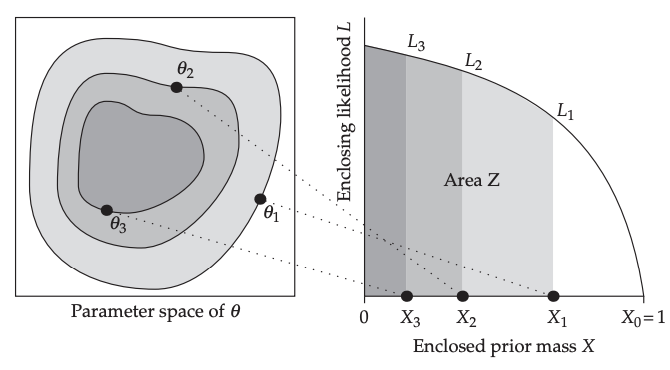
\includegraphics[width=0.5\linewidth]{Nested_lkhd_contours.png}
    \caption*{Nested likelihood contours sort to enclosed prior mass $X$}
\end{figure}

\subsection{The algorithm}

The basic nested sampling algorithm is:

\begin{enumerate}
    \item Draw $N_{\mathrm{live}}$ \textit{live points} from the prior. This corresponds to $X_0=1$:
    \begin{equation*}
        X_0=1=\int\pi(\theta)\,d\theta.
    \end{equation*}
    that is, there is no constraint on $L(\theta)$, and $X_0=1$ is the total prior mass. Initialise evidence $Z=0$.


    
    \item At iteration $i$, find the live point with the smallest likelihood, say $L_i^*$, and kill it.
    \item Estimate the compression factor
    \begin{equation*}
        t_i=\frac{X_i}{X_{i-1}},
    \end{equation*}
    where
    \begin{equation*}
        X_i = \int_{L(\theta)>L^*_i}\pi(\theta) d\theta.
    \end{equation*}
    Note that we have $X_0>\cdots>X_{i-1}>X_i>\cdots$.
    \item Add 
    \begin{equation*}
        \Delta Z_i = L_i^*(X_{i-1}-X_i)=L^*_i(1-t_i)X_{i-1}
    \end{equation*}
    to the evidence. Essentially, this step is an estimation of
    \begin{equation*}
        \int_{X_{i}}^{X_{i-1}}L(X)dX.
    \end{equation*}
    \item Replace the killed point by a new point drawn from the prior subject to the likelihood constraint
    \begin{equation*}
        L(\theta)>L_i^*.
    \end{equation*}
    \item Repeat 2-5 until the remaining contribution to the evidence is negligible.
    \item Suppose we run steps 2-5 for $T$ times. Add final evidence estimate of remaining live points:
    \begin{equation*}
        \Delta Z=\bar LX_{\mathrm{T}},
    \end{equation*}
    where $\bar L$ is the average of the likelihood of the live points, $X_T$ is computed in step 3 of the $T$-th run. 
\end{enumerate}

Now, let $\theta_i$ denote the dead point in $i$-th iteration. Then we can approximate the posterior by a weighted discrete distribution
\begin{equation*}
    P(\theta\mid D)\approx\sum_{i=1}^T w_i\delta_{\theta_i}(\theta),
\end{equation*}
where $\delta_{\theta_i}(\theta)$ denotes a point mass at $\theta=\theta_i$.

The weights can be approximated by
\begin{equation*}
    w_i=\frac{L_i^\star (X_{i-1}-X_i)}{Z}.
\end{equation*}

Indeed, since
\begin{equation*}
    P(\theta\mid D)=\frac{P(D\mid\theta)P(\theta)}{\int P(D\mid\theta)P(\theta)\,d\theta}=\frac{L(\theta)\pi(\theta)}{Z},
\end{equation*}
and in the discrete approximation, we have $L(\theta_i)=L^*_i$ by step 2. Also, each killed point lies in the range $L^*_{i-1}\le L(\theta_i)\le L^*_i$, so it covers a shell of the prior with size approximately $X_{i-1}-X_i$.

\subsection{Estimating the compression factor}


Consider steps 2-3 of iteration $i+1$, where a new live point is sampled in iteration $i$, with the ``surviving region''
\begin{equation*}
A_i:=\{\theta: L(\theta)>L_i^*\}.
\end{equation*}
The prior mass on $A_i$ is
\begin{equation*}
X_i=\int_{A_i} \pi(\theta)\,d\theta.
\end{equation*}

In nested sampling, each live point at this stage is distributed according to the
prior conditioned on \(A_i\). Hence its density is
\begin{equation*}
p_i(\theta)
=
\frac{\pi(\theta)\mathbf{1}_{A_i}(\theta)}{X_i}.
\end{equation*}
Now define the random variable
\begin{equation*}
Y:=X(L(\Theta)),
\qquad \Theta\sim p_i.
\end{equation*}
\textbf{Claim}: $Y\sim \mathrm{Unif}(0,X_i)$.

\begin{proof}
    Let $y\in[0,X_i]$. Then
\begin{equation*}
\mathbb{P}(Y\le y)
=
\mathbb{P}\bigl(X(L(\Theta))\le y\bigr).
\end{equation*}
Since $X(\lambda)$ is decreasing in $\lambda$, there exists a likelihood level
$\lambda(y)$ such that
\begin{equation*}
X(\lambda(y))=y.
\end{equation*}
Therefore, up to boundary sets of prior measure zero, the event
\begin{equation*}
\{X(L(\Theta))\le y\}
\end{equation*}
is equivalent to
\begin{equation*}
\{L(\Theta)\ge \lambda(y)\}.
\end{equation*}
Hence
\begin{equation*}
\mathbb{P}(Y\le y)
=
\mathbb{P}\bigl(L(\Theta)\ge \lambda(y)\mid \Theta\in A_i\bigr).
\end{equation*}
Using the conditional density $p_i$, we obtain
\begin{equation*}
\mathbb{P}(Y\le y)
=
\frac{\displaystyle \int_{L(\theta)\ge \lambda(y)}
\pi(\theta)\mathbf{1}_{A_i}(\theta)\,d\theta}{X_i}.
\end{equation*}
Now $y\le X_i$, so the contour $\{L\ge \lambda(y)\}$ lies inside the current
surviving region $A_i$. Thus
\begin{equation*}
\mathbf{1}_{A_i}(\theta)=1
\qquad\text{on }\{L(\theta)\ge \lambda(y)\},
\end{equation*}
and therefore
\begin{equation*}
\mathbb{P}(Y\le y)
=
\frac{\displaystyle \int_{L(\theta)\ge \lambda(y)} \pi(\theta)\,d\theta}{X_i}.
\end{equation*}
By the definition of $X(\lambda)$, we have
\begin{equation*}
\int_{L(\theta)\ge \lambda(y)} \pi(\theta)\,d\theta = y,
\end{equation*}
again up to boundary sets of prior measure zero. Hence
\begin{equation*}
\mathbb{P}(Y\le y)=\frac{y}{X_i},
\qquad 0\le y\le X_i.
\end{equation*}
\end{proof}





The worst point corresponds to the highest $X$ of $N_{\mathrm{live}}$ uniform draws, so
\begin{equation*}
    t_i=\frac{X_i}{X_{i-1}}
\end{equation*}
has  $\mathrm{Beta}(N_{\mathrm{live}},1)$ distribution, that is
\begin{equation*}
    P(t_i)=N_{\mathrm{live}}\,t_i^{\,N_{\mathrm{live}}-1},
    \qquad 0<t_i<1.
\end{equation*}
We approximate $\ln t_i$ by its mean:
\begin{equation*}
    \ln t_i\approx\mathbb{E}[\ln t_i]=-\frac{1}{N_{\mathrm{live}}},
\end{equation*}
so we get the approximation
\begin{equation*}
    t_i \approx e^{-1/N_{\mathrm{live}}}.
\end{equation*}


\section{Variational inference}


Sampling methods such as MCMC and nested sampling can be slow, although they give exact samples in the long-run. \textit{Variational inference} takes a different approach: instead of trying to get exact samples, we seek a simple approximation to the posterior that is close enough for practical purposes.

\textit{Variational Bayes} treats Bayesian inference as an optimisation problem. We choose a family of approximating distributions
$\mathcal{Q},$
and seek the best
$q(\theta)\in \mathcal{Q}$
to approximate the posterior
$P(\theta\mid D).$

\subsection{Kullback--Leibler divergence}

To measure the ``closeness'' between distributions, we use the \textit{Kullback--Leibler divergence}
\begin{equation*}
    \mathrm{KL}(q(\theta)\,\|\,p(\theta))
    =
    -\int q(\theta)\ln\!\left(\frac{p(\theta)}{q(\theta)}\right)d\theta.
\end{equation*}
Note that $\mathrm{KL}(q\|p)=0$ iff $q(\theta)=p(\theta)$ for all $\theta$, and $\mathrm{KL}(q\|p)>0$ otherwise. Also, KL divergence is not symmetric:
\begin{equation*}
    \mathrm{KL}(q(\theta)\|p(\theta))
    \neq
    \mathrm{KL}(p(\theta)\|q(\theta)).
\end{equation*}

\subsection{Variational families}

Variational inference chooses the best approximator inside a restricted family $\mathcal{Q}$. Common choices include:

\paragraph{Multivariate Gaussian with full-rank covariance}
\begin{equation*}
    q(\theta)=\mathcal{N}(\theta\mid \mu_q,\Sigma_q).
\end{equation*}

\paragraph{Uncorrelated Gaussian}
\begin{equation*}
    q(\theta)=\mathcal{N}(\theta\mid \mu_q,\mathrm{diag}(\sigma_q^2)).
\end{equation*}

\paragraph{Mean-field}
\begin{equation*}
    q(\theta)=\prod_{i=1}^m q_i(\theta_i).
\end{equation*}


\subsection{Finding the best approximator}

The aim is to find
\begin{equation*}
    q^\star(\theta)
    =
    \arg\min_{q\in \mathcal{Q}}
    \mathrm{KL}\!\bigl(q(\theta)\,\|\,P(\theta\mid D)\bigr).
\end{equation*}

Note that
\begin{align*}
    \mathrm{KL}\!\bigl(q(\theta)\,\|\,P(\theta\mid D)\bigr)
    &=
    -\int q(\theta)\ln\!\left(\frac{P(\theta\mid D)}{q(\theta)}\right)d\theta\\
    &=
    \int q(\theta)\ln q(\theta)\,d\theta
    -
    \int q(\theta)\ln P(\theta\mid D)\,d\theta\\
    &=
    \mathbb{E}_q[\ln q(\theta)]
    -
    \mathbb{E}_q[\ln P(\theta\mid D)].
\end{align*}
Now write the posterior as
\begin{equation*}
    P(\theta\mid D)=\frac{P(\theta,D)}{P(D)},
\end{equation*}
then
\begin{align*}
    \mathrm{KL}\!\bigl(q(\theta)\,\|\,P(\theta\mid D)\bigr)
    &=
    \mathbb{E}_q[\ln q(\theta)]
    -
    \mathbb{E}_q[\ln P(\theta,D)]
    +
    \ln P(D).
\end{align*}
Rearranging gives
\begin{equation*}
    \ln P(D)
    =
    \mathrm{KL}\!\bigl(q(\theta)\,\|\,P(\theta\mid D)\bigr)
    +
    \mathrm{ELBO}(q),
\end{equation*}
where
\begin{equation*}
    \mathrm{ELBO}(q)
    =
    \mathbb{E}_q[\ln P(\theta,D)]
    -
    \mathbb{E}_q[\ln q(\theta)].
\end{equation*}
The quantity $\mathrm{ELBO}(q)$ is the \textit{evidence lower bound}. Since KL divergence is nonnegative, we have
\begin{equation*}
    \ln P(D)\ge \mathrm{ELBO}(q).
\end{equation*}


Moreover, because $\ln P(D)$ does not depend on $q$, minimizing the KL divergence is equivalent to maximizing the ELBO:
\begin{equation*}
    q^\star
    =
    \arg\min_{q\in\mathcal{Q}}
    \mathrm{KL}\!\bigl(q(\theta)\,\|\,P(\theta\mid D)\bigr)
    =
    \arg\max_{q\in\mathcal{Q}} \mathrm{ELBO}(q).
\end{equation*}
Equivalently,
\begin{equation*}
    q^\star
    =
    \arg\max_{q\in\mathcal{Q}}
    \left\{
    \mathbb{E}_q[\ln P(\theta,D)]
    -
    \mathbb{E}_q[\ln q(\theta)]
    \right\}.
\end{equation*}
Note that this allows us to optimise $q$ without computing the exact evidence $P(D)$.







\end{document}